\documentclass{mpaper}
\usepackage{enumitem}
\usepackage{amsthm}
\usepackage{thmtools}
\usepackage[numbers]{natbib}
\usepackage{multicol}
\usepackage{graphicx}
\usepackage{subcaption}

\newcommand{\specialcell}[2][c]{%
  \begin{tabular}[#1]{@{}c@{}}#2\end{tabular}}

\def\Item$#1${\item[] $\displaystyle#1$
   \hfill\refstepcounter{equation}(\theequation)}

\newtheorem{example}{Example}
\newtheorem{theorem}{Theorem}

\declaretheoremstyle[headfont=\normalfont]{normalhead}
\declaretheoremstyle[headfont=\bfseries]{boldhead}
\declaretheorem[style=boldhead, numbered=no]{question}
\declaretheorem[style=boldhead, numbered=no]{instance}


\begin{document}

\title{Algorithms for Multi-City Travel Itineraries}
\author{Iva Babukova}
\matricnum{2030458b}

\maketitle

\begin{abstract}

The Traveller's Problem (TP) is a combinatorial optimisation problem that is often encountered by travellers around the world. Given a set of airports, a set of flights, a set of destinations that is a subset of the airports, and a home airport $A_{0}$, a solution is a travel schedule that starts and finishes at $A_{0}$, visits all destinations and is in accordance with additional constraints specified by the traveller. These may require spending a certain amount of days in each destination or taking a minimum number of connecting flights for example.
The review of existing literature indicates that TP is unlikely to have been studied: we were unable to find a formal description of TP or an attempt to solve it. This work formally defines TP and constructs two solutions for the problem using Integer Programming (CP) and Constraint Programming (CP). We also build a framework for creating TP instances using flight data given by a flight metasearch engine called Skyscanner. The evaluation of the models shows that the IP model is faster then the CP model for all instances. The results further suggest that both models are not efficient enough to be used as part of a real-time flight booking platform: the number of flights in the instance has significant impact on the running time of the algorithms. We suggest ways to improve the performance of the models that can be carried out as part of future work.
\end{abstract}

\section{Introduction}
\label{intro}
\subsection{Problem Motivation}
Online travel planning is the process of booking holidays over the Internet using one or more websites that offer details about available itineraries. It is one of the fastest growing sectors in the travel industry. \cite{onlinetransportbooking}. At the moment, online booking systems provide no efficient solutions for finding itineraries involving multiple cities. If a traveller wants to visit several destinations with unspecified order and dates, they have to manually query for all permutations of dates and destinations in order to find the best trip. This easily turns into an intractable task and travellers are often forced to book suboptimal trips.

TP can be classified as a member of the family of routing problems. \textit{Routing Problems} are a set of problems within the area of combinatorial optimisation and operational research that ask for an optimal route through a set of destinations that satisfies all time window, capacity and any additional instance-specific constraints. Examples of routing problems are the Travelling Salesman Problem (TSP) and the Vehicle Routing Problem (VRP). Routing problems find direct applications in multiple areas: transportation and logistics \cite{Flood56}, planning inspections of remote sites \cite{Mahalanobis}, genome sequencing \cite{genomesequencing}, data clustering \cite{McCormick72} and many others.

This work is organised as follows. Section \ref{npcompleteproblems} formulates TP and other routing problems discussed throughout this work. Existing work is presented in Section \ref{existingwork}. The design and implementation of the TP algorithms and the TP instance generator are discussed in Section \ref{tpmodels} and Section \ref{skyscannerdata} respectively. Section \ref{evaluation} presents the empirical analysis of the algorithms. Section \ref{conclusionandfuturework} presents a summary of this work, gives suggestions for improvement and proposes future directions this project can take.

\subsection{Routing Problems Formulations}
\label{npcompleteproblems}

This section includes formulations of TP and two existing NP-hard \citep{thebible} routing problems studied throughout this work, namely the Travelling Salesman Problem and the Vehicle-Routing Problem.

\subsubsection{Vehicle-Routing Problem (VRP)}
\begin{instance}
A set $A$ of $n$ cities, where $D \in A$ is the \textit{depot} and each city $i$ has demand $c_{i}$, a fleet of $m$ vehicles $V$, where vehicle $k$ has capacity $q_{k}$, a distance $d(i,j)$ between two cities $i$ and $j$ and a positive integer $B$.
\end{instance}

\begin{question}
Is there a set $\mathcal{S}$ consisting of $m$ sequences $s_{1},...,s_{m}$, of the cities in $A$, called \textit{tours}
where for every vehicle $k$ $(1 \leq k \leq m)$:
\begin{itemize}
\vspace{-1mm}
\item $s_{k} = \langle A_{s_{k,1}},...,A_{s_{k,p_{k}}} \rangle$, \quad where $p_{k}$ is the number of the cities in the tour of $k$,
\item $\sum_{i = 1}^{p} c_{A_{s_{k,i}}} \leq q_{k}$,
\item $A_{s_{k,1}} = D$,
\item $s_{i} \cap s_{j} = \{D\}$, \quad $(1 \leq i < j \leq m),$
\item $s_{1} \cup s_{2} ... \cup s_{m} = A$,
\end{itemize}
and
\vspace{-1mm}
$$ \sum_{k=1}^{m} C(s_{k}) \leq B \textrm{, where } $$
\vspace{-1mm}
$$C(s_{k}) = \bigg( \sum_{i=1}^{p_{k}} d(A_{s_{k,i}}, A_{s_{k,i+1}}) \bigg) + d(A_{s_{k,k_{p}}}, A_{s_{k,1}}) \textrm{ ?}$$
\end{question}

\subsubsection{Travelling Salesman Problem (TSP)}
\begin{instance}
Set $A$ of $n$ cities, distance $d(A_{i}, A_{j})$ between each pair of cities $A_{i}$, $A_{j}$ $\in$ $A$, positive integer $B$.
\end{instance}

\begin{question}
Is there a tour of $A$ having length $B$ or less, i.e., a permutation of cities $\gamma = \langle A_{\pi_{1}},...,A_{\pi_{n}} \rangle $ of $A$ such that the total travel distance $L_{\gamma}$:
\vspace{-1mm}
$$L_{\gamma} = \bigg( \sum_{i=1}^{n-1} d(A_{\pi_{i}}, A_{\pi_{i+1}}) \bigg) + d(A_{\pi_{n}}, A_{\pi_{1}}) \leq B \quad \textrm{?}$$
\end{question}

Note that TSP is a special case of VRP when only one vehicle is allowed.

\subsubsection{Traveller's Problem (TP)}
\begin{instance}
Each instance of TP consists of:

\begin{itemize}[topsep=0.1em]
\setlength\itemsep{0.1em}
\item A set of airports $A = \{ A_{0},...,A_{n} \}$ for $n > 0$. Each airport $A_{i}$ $\in$ $A$ represents a location the traveller can begin their trip in, visit as a desired destination, or connect in on the way to their destination.

\item A set of \textit{destinations} $D = \{ D_{1},...,D_{l} \}$, $D \subseteq A$, $l \leq n$.

\item The trip starts and ends at the same airport $A_{0}$, which is referred to as the \textit{home airport}.

\item The total travel time $T$, within which the traveller must have visited all destinations and returned to the home airport. The first day is day 0.
 
\item A set of flights $F = \{ f_{0},...,f_{m-1} \}$. Each flight $f_{j}$ has a departure airport $A^{d}_{j}$, an arrival airport $A^{a}_{j}$, date $t_{j}$, duration $\Delta_{j}$, cost $c_{j}$,
for some non-negative integer $j$ less than or equal to $n$.
The date $t_{j}$ is a positive rational number less than or equal to $T$ that shows at which day $f_{j}$ leaves its departure airport. The duration $\Delta{j}$ is a positive fraction that shows the amount of time that takes for flight $f_{j}$ to go from $A^{d}_{j}$ to $A^{a}_{j}$. The cost $c_{j}$ is a positive number that denotes the number of units of some currency $\epsilon$ that the traveller pays in order to be able to board flight $f_{j}$.

\item Each airport $A_{i}$ has \textit{connecting time} $C_{A_{i}}$, that is the time that takes to switch from any selected flight $f_{p}$ with $A^{a}_{p} = A_{i}$ to any selected flight $f_{q}$ with $A^{d}_{q} = A_{i}$, where $f_{q}$ is immediately after $f_{p}$ in a solution.
\end{itemize}
\end{instance}

\begin{question}
Is there a sequence $s \subseteq F$ of $k$ valid flights: $s = \langle f_{i_{1}},...,f_{i_{k}} \rangle $, referred to as a \textit{trip}, where the flights in $s$ satisfy the following \textit{trip properties}:

\begin{enumerate}[topsep=0.3em]
\setlength\itemsep{0.3em}
\item $A^{d}_{i_{1}} = A^{a}_{i_{k}} = A_{0}$,
\item $ A^{a}_{i_{j}} = A^{d}_{i_{j+1}},  \quad 0 < j < k$,
\item $ t_{i_{j}} + \Delta_{i_{j}} + C_{r} \leq t_{i_{j+1}}, \quad 0 < j \leq k, \quad r = A^{d}_{i_{j+1}}$,
\item $t_{i_{k}} + \Delta_{i_{k}} \leq T$,
\item $ \forall D_{p} \in D, \textrm{ } \exists \textrm{ } f_{i_{j}} \in s \textrm{, such that } A^{a}_{i_{j}} = D_{p}$.
\end{enumerate}
Note that $s$ may contain one or more flights to and from airports that are not destinations. Such airports are called \textit{connecting airports}. Flight that either departs from or arrives at connecting airport is called \textit{connecting flight}.
\end{question}
% todo: say that this work studies the optimisation version of TP
The \textit{optimisation} version of TP (TPO) asks for an \textit{optimal} solution $opt(s)$ of $s$ with respect to a given objective function. The objective function may minimize or maximise on connecting airports, cost, travel duration or the number of flights in $s$.

The \textit{decision} version of TP (TPD) asks whether there exists a valid sequence of flights $s$, such that some properties of $s$ have values less than or equal to a given integer $B$. TPD is shown to be is NP-complete (Appendix \ref{appendix:tpcomplexity}), from which it follows that TPO is NP-hard.

This problem formulation has only presented the constraints which every trip must satisfy. In reality, travellers may have additional preferences with regards to their travel. These are discussed in the next two sections.

\subsubsection*{Hard Constraints}
\label{subsec:hardconstraints}
Additional constraints might be imposed on an instance of TP. A solution that does not satisfy all required constraints is considered invalid. Examples of hard constraints include:

\begin{enumerate}[topsep=0.1em]
\setlength\itemsep{0.1em}
\item Travellers may wish to spend a certain amount of days at a given destination, specified by both upper and lower bounds. The days may additionally be constrained to be consecutive or not.

\item Travellers may require to spend a given date at a given destination, for example due to an event occurring on that date in this destination.

\item Travellers may require not to fly through a given airport more than once.
\end{enumerate}

\subsubsection*{Soft Constraints}
\label{subsec:softconstraints}
It may be desirable to search for solutions that satisfy some requirements, but still accept trips that violate them. Such requirements are called \textit{soft constraints} and for TP they can be some of the following:

\begin{enumerate}[topsep=0.1em]
\setlength\itemsep{0.1em}
\item Travellers may wish to spend a certain amount $\delta_{i}$ of days in each destination $D_{i}$, where $\delta_{i}$ may be specified as a lower or an upper bound.

\item Travellers may wish to avoid taking connecting flights. In such requirement, we wish to maximise the number of flights to and from destinations.

\item Travellers may want to spend as little time on flying as possible. In such case, we wish to find a solution that minimises the sum of the durations of all flights.
\end{enumerate}

%% mention the problem with lexicographic optimisation and multi-objective opimisation
Note that there may exist an instance for which all soft constraints can not be satisfied simultaneously. In such case, the traveller may be required to rank their requirements in an order of preference. The instance becomes a lexicographic optimisation problem, where the highest ranked objective is optimised first, then the next highest ranked objective and so on. If all requirements are equally important for the traveller, the instance becomes a multiobjective optimisation problem, where the objectives are all constraints required by the traveller. Each of the objectives is assigned a weight of influence on the final solution set. The problem is then to optimize the objective function, composed by the constraints, each of them multiplied by its weight. Multiobjective optimisation is further investigated in this work.

Most of the constraints presented in this section can be viewed as either hard or soft, depending on the user requirements. Therefore this work assumes as an additional non-functional requirement that any constructed TP models are flexible and easy to extend by adding, removing and modifying constraints and objective functions. The choice of techniques for solving TP, discussed later in this work, is highly influenced by this requirement.

\section{Existing Work}
\label{existingwork}

This section is a discussion of two widely used methods for solving routing problems: Integer Programming (IP) and Constraint Programming (CP) and the principles of Branch and Bound methods, typically employed as IP and CP search algorithms. The background of the real-world data used for generating TP instances is also discussed.

\subsection{Integer Programming}
\label{sec:ip}

Integer Programming (IP) is a way to solve optimisation problems by modelling their requirements as linear inequalities and equations, called \textit{constraints}, where variables are restricted to take only integer values. Optimal solutions are obtained by optimising an \textit{objective function} subject to the constraints. This task is done by an IP \textit{solver}, which incorporates implementations of some specialised search algorithms. Solving a problem with IP requires building a suitable model and passing it to the IP solver. There is a range of solvers one can use.

The next section presents an example IP model of the Travelling Salesman Problem (TSP), defined in Section \ref{npcompleteproblems}, constructed by \citet{Dantzig54}.

\subsubsection*{Dantizg, Fulkerson and Johnson}
%\citet{Dantzig54} formulate TSP as the following IP problem.
Let $x(i,j)$ be a variable that denotes whether city $j$ immediately succeeds city $i$ in a TSP tour. The value of $x(i,j)$ is equal to 1 if this is true, or 0 otherwise. If $x(i,j)$ is 1, then $i$ is called an \textit{outgoing} city and $j$ - an \textit{incoming} city. The objective function of TSP is to minimise the total length of the tour, which \citet{Dantzig54} express as the following function:

\vspace{-1mm}
\begin{equation}
\label{eq:objfunc}
\vspace{-1mm}
\textrm{min } \sum_{i\in A}\sum_{j\in A} d(i,j)x(i,j) \textrm{,}
\end{equation}

where $A$ is the set of all cities and $d(i,j)$ is the distance between cities $i$ and $j$.

In each TSP tour every city has to be visited once, i.e each city has to be incoming and outgoing exactly once. This can be enforced with the following constraint:

\vspace{-1mm}
\begin{equation}
\label{eq:one}
\begin{split}
  \sum_{j \in A} x(i,j) = 1, \qquad i \in A,\\
  \sum_{i \in A} x(i,j) = 1, \qquad j \in A,
\end{split}
\end{equation}
\vspace{-1mm}

Constraint (\ref{eq:one}) ensures that each city in $A$ is picked exactly once as an incoming and an outgoing city. However, it allows for the existence of one or more cycles of $n_{1} < n$ cities, called \textit{subtours}, where some cities are visited more than once. For example, consider Figure \ref{fig:tour} and Figure \ref{fig:subtours}. Both of them satisfy constraint (\ref{eq:one}), but Figure \ref{fig:subtours} does not represent a valid tour, because it contains two subtours, each of size 3. To tackle this problem, \cite{Dantzig54} introduce the \textit{subtour elimination} constraint:

\vspace{-1mm}
\begin{equation}
\label{eq:subtourElimination}
\begin{split}
\sum \{x(i,j) : (i,j) \in (S \times \bar{S}) \cup (\bar{S} \times S)\} \geq 2,\\ 
\forall \, \emptyset \subset S \subset A, \textrm{ where } \bar{S} = A \setminus S
\end{split}
\end{equation}
\vspace{-1mm}

Here, $S$ is a subset of A and $\bar{S}$ is the set of all cities that are in $A$ and not in $S$. Constraint (\ref{eq:subtourElimination}) enforces that at least two cities in $S$ are connected with cities from $\bar{S}$. Figure \ref{fig:tour} and Figure \ref{fig:subtours} serve as examples. Let $S = \{A_{1},A_{2},A_{3}\}$, then $\bar{S} = \{A_{4},A_{5},A_{6}\}$. Constraint (\ref{eq:subtourElimination}), would detect the tour on Figure \ref{fig:subtours} as invalid, as there is no city in $S$ that is connected to a city in $\bar{S}$. Figure \ref{fig:tour} will be accepted, since $A_{1}$ and $A_{3}$ are connected with $A_{6}$ and $A_{4}$ respectively.

\begin{figure*}
\centering
\begin{minipage}{.5\textwidth}
  \centering
  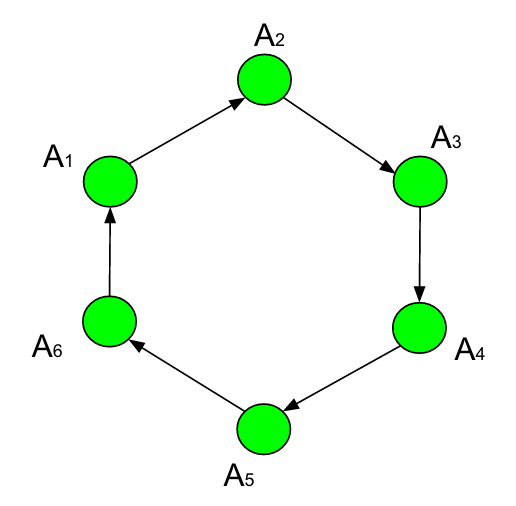
\includegraphics[width=3cm, height=3cm]{images/valid.png}
  \caption{A valid TSP tour}
  \label{fig:tour}
\end{minipage}%
\begin{minipage}{.5\textwidth}
  \centering
  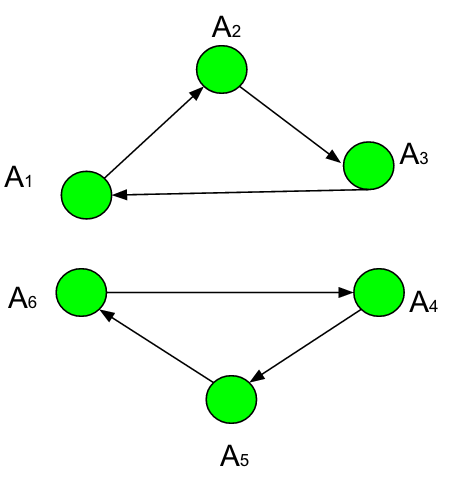
\includegraphics[width=3cm, height=3cm]{images/invalid.png}
  \caption{Two subtours of size 3}
  \label{fig:subtours}
\end{minipage}
\end{figure*}

Solving TSP is done by minimising the objective function (\ref{eq:objfunc}), subject to constraints (\ref{eq:one}) and (\ref{eq:subtourElimination}).

\citet{Dantzig54} solve this TSP IP model using a novel methods for that time, such as the \textit{cutting-plane} method and the \textit{assignment problem relaxation}, where the latter is discussed in the next section. We point the interested reader to \cite{Dantzig54} and \cite{Dantzig59}, where the cutting-plane method is explained in more detail using a 10 city TSP instance as an example.

Other example solutions of routing problems with IP include \cite{Achuthan91, Baker83}. \citet{Achuthan91} give an IP formulation for the VRP.
\citet{Baker83} presents a model for the Time-Constrained TSP (TCTSP), defined in Section \ref{npcompleteproblems}. TCTSP is modelled as a system of linear integer inequalities, solved by a branch and bound procedure with bounds calculated using an algorithm for the longest path problem \footnote{The longest path problem is the problem of finding a path of maximum length in a graph with no repeated vertices.}. 

\subsection{Constraint Programming}
\label{sec:cp}
Constraint Programming (CP) is an alternative method for solving optimisation problems. Similarly to IP, CP first requires building a model of the problem. Modelling a problem instance $\pi$ yields a constraint satisfaction problem (CSP) $CSP(\pi)$, which consists of a set of decision variables $V$, a set of rules, called \textit{constraints} concerning the assignment of values to variables and an \textit{objective}. Unlike IP, CP constraints need not be linear integer inequalities. Moreover, CP supports specialised constraints like ``if-then'' and ``all-different''. Each variable in $V$ has a set of possible values, called \textit{domain}. A \textit{solution} to $\pi$ is an assignment of each variable in $V$ to a value in its domain, such that all constraints are satisfied and the objective is optimised. The program that searches for a solution $CSP(\pi)$ is called a \textit{solver}. Similarly to IP, implementing a CP solver is not needed.

The remaining of this section discusses existing formulations of some routing problems as CSPs.

\subsubsection*{TSP with CP}
We present an alternative approach to model TSP using CP. The technique is developed by \citet{Caseau97} and it can handle small to medium size problem instances with size equal to 40 cities on average. \citet{Caseau97} motivate the choice of this size by arguing that it is both frequently encountered in practice and not extensively studied.

%%%% CP model, branching rule, bounding rules
The $CSP(TSP)$ constructed by \citet{Caseau97} is similar to the TSP IP model discussed in the previous section. Let the set of cities $A$ be duplicated into two sets $A_1$ and $A_2$. \citet{Caseau97} represent each city $i \in A_1$ as a variable with domain equal to all cities in $A_2$ that are not equal to $i$. The assignment $i = j$, $i \in A_1$, $j \in A_2$ implies that the next visited city after $i$ is $j$. The assignment of values in $A_2$ to variables in $A_1$ is equivalent to a bipartite perfect matching from $A_1$ to $A_2$ \cite{Caseau97}, which has the same effect as constraint (2) from the TSP IP model.

%%%% subtour elimination
Subtour elimination is imposed by restricting the domains of certain variables upon each assignment \cite{Caseau97}. Whenever variable $i$ is assigned the value $j$, all paths adjacent to cities $i$ and $j$ are checked. Let $x$ be a path that ends in $i$ and $y$ be a path that starts from $j$. If $|x| + |y| < n-2$, then the variable at the end of $y$ can not be assigned the city at the start of $x$ as value, because that would lead to a cycle of size less than $n$.

\citet{Caseau97} also introduce a \textit{lookahead} technique that predicts when certain partial variable assignments will inevitably lead to an invalid tour. The technique detects assignments that are necessary to enforce the cyclic property of a TSP tour and marks as invalid all partial assignments that do not satisfy these properties.

%Rules that determine the next variable that is to be assigned a value are called \textit{branching rules} and they are a type of heuristics, commonly added to CSPs and used as part of a branch and bound algorithm. A \textit{heuristic} is a ``rule of thumb'' that ``guides'' the search and aims to limit the total space explored by a search algorithm. Previous work has shown that heuristics can potentially reduce the search effort significantly \cite{Haralick80:a, Gent96,Christopher03}.

%The fail-first principle \citep{Haralick80}  is a heuristic that chooses as next variable the one which is most likely going to lead to a domain wipeout. Let $a$ and $b$ be the two cities closest to some city $i$. The \textit{regret} of $i$, is equal to the distance between $a$ and $b$, that is $d(a,b)$. \citet{Caseau97} propose several combinations of largest regret and fail-first principle-based heuristics as branching rules.

\citet{Caseau97} prune suboptimal partial solutions by imposing a lower bound on the tour distance, which is the sum of the distances between each city $i$ and the city nearest to $i$. The authors also use this bound for pruning values from the domain of some variables. For instance, when $d(i,j)$ has a value that is much higher than the best assignment for $i$ and $j$, the procedure predicts that the assignment $i = j$ would inevitably fail.

\citet{Caseau97} note that CP is a ``truly flexible approach'', where flexibility is defined as the ability to easily add or remove extra constraints to the initially constructed model. For instance, one can represent TSP with time windows by only adding few more constraints to the TSP CSP constructed above. This flexibility of CP has been noted before \cite{Kilby00, Pesant1997}.

Other CP algorithms for routing problems include GENIUS-CP \citep{Pesant1997}, \citet{Backer2000} and \citet{rousseau2002solving}.
GENIUS-CP \cite{Pesant1997} is a combination of novel vehicle routing heuristics and a CP model for VRP. The model can be easily adapted to solve problems from many different contexts by exploiting the flexibility of CP. \citet{Backer2000} also construct a CP model for VRP and use iterative improvement techniques and heuristics to speed up the search. \citet{rousseau2002solving} use an approach that combines CP with the column generation method introduced by \citet{dantzig1960decomposition}. Their method targets VRPs with time window constraints.

\subsection{Branch and Bound methods}
% On the optimisation engine level, after each decision on assignment of values to values, CP performs logical inference to reduce the available options for the remaining variables' domains. In contrast, IP uses a combination of relaxations, a specialised optimisation refinement method, called \textit{cutting-planes} \cite{Dantzig54} and a \textit{branch and bound} \cite{Little63} search technique. A CP engine proves optimality by showing that no better solution than the current one can be found, whereas an IP engine uses a linear relaxation with bounds and cuts proof.

The term ``branch and bound'' was first coined by \citet{Little63} and it refers to a widely-used method for solving optimisation problems. Branch and bound algorithms are one of the most successful methods for solving optimisation problems \citep{Christofides81} and they are typically implemented in Constraints Programming (CP) and Integer Programming (IP) solvers \citep{Atamturk2005,Leyffer01,Quesada92}.

A branch and bound algorithm iteratively divides the current set of problems into successively smaller subsets, called \textit{subproblems}, calculates bounds on their values and discards subproblems that would lead to suboptimal solutions. After the termination of the algorithm, the best solution found so far is considered an optimum. %The search performed by a branch and bound algorithm can be represented as the tree shown in Figure \ref{fig:bandb}. The root node represents the original problem, which is then divided into two smaller subproblems. Each subproblem is the \textit{child} of the problem it was derived from. If the bounds on the values of a subproblem pass required bounding constraints, then the subproblem is further divided.

% \begin{figure}
% \centering
% \includegraphics[width = 4cm, height = 3cm]{images/bandb.png}
% \caption{Branch and bound search tree}
% \label{fig:bandb}
% \end{figure}

Branch and bound algorithm iterates over the entire solution space. However unlike exhaustive search, the use of bounds on the value of optimal solutions enables the algorithm to provably ignore parts of the search space.
%explore some parts of the solution space only implicitly.

The process of dividing each solutions set into subproblems is called \textit{branching}. The choice of bounding and branching procedures is shown to be crucial to the size of the explored search space \citep{Little63,Dantzig54, HeldK70}. Existing literature has spent substantial effort in constructing efficient algorithms for branching and bounding. Some of these algorithms are discussed in this section.

\subsubsection*{Branching Strategies}
Branching algorithms can be based on either \textit{variable} or \textit{node} selection. Variable selection strategies are rules about how to divide the current set of solutions into subproblems, so that they are easier to solve than the original problem. Node selection methods choose which set of solutions should be branched next.

Common branching strategies estimate the impact of the variables on the objective functions or on the constraints. For example the next variable to branch on can be the one that imposes highest or lowest number of restrictions.
We point the interested reader to the works of \citet{Atamturk2005} and \citet{Achterberg}, which discuss most common branching strategies and evaluate their influence on the performance of the branch and bound algorithm.

\subsubsection*{Calculating Bounds}
Relaxations are commonly used bounding strategies. A \textit{relaxation} of a problem $\pi$ is the process of obtaining another problem $\pi^\prime$ that is believed to be easier to solve by removing some constraints from $\pi$, where a feasible solution in $\pi$ maps to a feasible solution in $\pi^\prime$, but the converse need not be true in general. Solutions to $\pi^\prime$ give information about the lower or the upper bound of the values of $\pi$.

Some examples of relaxations include the Assignment Problem (AP) relaxation, the Lagrangian relaxation and the Set Partitioning Problem (SPP) relaxation. The AP relaxation consists of removing the subtour elimination constraint from the TSP IP model defined in Section \ref{sec:ip} and minimising the objective function (\ref{eq:objfunc}) only subject to constraint (\ref{eq:one}). The solution of the relaxed problem is used as a lower bound of the original problem. The AP relaxation is extensively used in the existing literature \cite{Fischetti92,Jonker80,Eastman58,Laporte86}.

The set partitioning problem (SPP) relaxation, discussed in the remainder of this section, is commonly used for VRP \citep{Desrochers92,Agarwal89,Desrosiers84,Alvarenga07}. It is performed as follows. Let $\mathcal{R}$ be the set of all feasible routes, where $c_{r}$ denotes the cost of a route $r \in R$. Let $\delta_{i,r}$ and $x_{r}$ be two variables that can be either 0 or 1. For each $r \in R$, $\delta_{i,r}$ is 1 if $r$ visits city $i$ and $x_{r}$ is 1 if $r$ is used in the solution. Then, VRP can be formulated as the problem of choosing a set $\mathcal{S} \subset R$ with minimal cost, known as the \textit{set partitioning problem} (SPP), that is:

\vspace{-1mm}
\begin{equation}
\label{eq:tcvrpobjfunc}
\textrm{minimise } \sum_{r \in R} c_{r} x_{r},
\end{equation}
\vspace{-3mm}

\begin{equation}
\label{eq:tcvrpconstraint1}
\sum_{r \in R} \delta_{i,r} x_{r} = 1, \quad \forall i \in A \setminus \{D\},
\end{equation}
\vspace{-1mm}

where constraint (16) imposes that each city is part of a set which is used in the solution. Some algorithms then construct a LP relaxation of this formulation and use the solution of the relaxation as a lower bound for a specific branch and bound procedure \citep{Desrochers92,Agarwal89}.

%Another well-known method for computing lower bounds is based on the minimum weight spanning tree and it is introduced by \citet{HeldK71} for TSP.


\subsection{Travel Booking Systems}
\label{sec:metasearchengines} 
A \textit{metasearch engine} queries multiple search engines and returns a ranked list of the aggregated results. A class of online booking systems work on top of a metasearch engines in order to help users find their desired itineraries. Given a query composed of home airport, destination, inbound and outbound dates, supplied by the traveller once, the travel metasearch engine returns a ranked list of all relevant flights.

\textbf{Skyscanner.} Skyscanner \cite{skyscanner} is a travel metasearch engine, available in over 30 languages and used daily by over 7.6 million people \cite{skyscannerusage}. Whenever the user clicks on one of the query results on the Skyscanner website \cite{skyscanner} in order to complete their booking, Skyscanner saves the information about the booking to a database. The data from all bookings is referred to as \textit{redirects data}.

Every booking $b_k$ in the redirects data contains a list of flights $H_k$ and their total price $c_k$, expressed as number of units of a some currency $\epsilon_k$. Each flight $f_{k_j}$ in $H_k$ has departure date $t_{k_j}$, arrival date $a_{k_j}$, departure airport $A^d_{k_j}$ and arrival airport $A^a_{k_j}$. Redirects data for half a year for the time period between 1$^{st}$ of July 2016 and 1$^{st}$ of January 2017 was given by Skyscanner for the empirical study and testing of the constructed CP and IP TP models. The data is of size 38 GB and it contains 321,465,401 unique bookings. The process of obtaining TP instances from the redirects data is presented in Section \ref{skyscannerdata}.

\section{Solutions to TP}
\label{tpmodels}
Two solutions to TP using IP and CP have been designed and implemented. This section presents the models, the choice of IP and CP solvers and the flights and airports representation.

\subsection{Data Structures}
The Java built-in implementation of a hash table, called \textit{HashMap} \cite{javahashmap}, is used for representing all flights and airports as follows.

Each flight $f_j$ is assigned an integer $k_j$, for $0 \leq k_j \leq m$ as a unique id and each airport $A_i$ has a unique code $c(A_i)$.

All flights are kept in a hash table $H_F$, where for each flight $f_j$, $k_j$ is a key and $A^d_j$, $A^a_j$, $t_j$, $\Delta_j$ and $c_j$ are the values associated with this key.

All airports are kept in three hash tables $H_A$ $H_d$ and $H_a$. For each $A_i \in A$, $H_A$ maps $c(A_i)$ to $C_{A_i}$. Hash tables $H_d$ and $H_a$ record the ids of the flights that depart from and arrive at each airport respectively, that is, for every $f_j \in F$, $k_j$ is recorded as a value associated with key $A^d_j$ in $H_d$, and again as a value associated with key $A^a_j$ in $H_a$.

This representation is used for both CP and IP models. Its choice is motivated by the fact that both models require frequent access to all departing or arriving flights for a given airport, as will be seen in the next two sections. This usage of HashMaps promises $\mathcal{O}(1)$ complexity for getting and putting elements for each hash table, provided that risks of rehashing are avoided \cite{javahashmap}. Since the number of flights and airports is specified on the first line of each TP instance, their sizes are known when the hash table is created and no rehashing occurs.

\subsection{ The CP model}
\label{subsec:tpcp}
The CP model for TP is constructed as follows.
Let $m = |F|$. The decision variables are an array $\mathcal{S}$ of size $m+1$ (indexed $0,1,...,m$) that represents the TP tour and a variable $z$ with domain $dom_{z} = \{1,...,m\}$ that denotes the number of flights in the trip. If $\mathcal{S}[i] = j$, then flight $f_{j} \in F$ is the $(i+1)^{th}$ flight in the tour, for $(0 \leq i < m)$ and $(1 \leq j \leq m)$. The end of the tour is marked by setting $\mathcal{S}[z] = 0$. All subsequent variables in $\mathcal{S}$ will then have to be 0. Each variable $v$ in $\mathcal{S}$ is either 0, if no flight is taken at that step, or it is equal to some flight number, that is $dom_{v} = \{0,...,m\}$.

\textbf{Constraints.} The constraints added to the model enforce the five trip properties and make $\mathcal{S}$ form a valid sequence of flights.

The following constraint restricts that once the end of the trip is reached at some position $z$, no flights are further added to $\mathcal{S}$.
\begin{itemize}
\Item
$\mathcal{S}[i] > 0 \wedge \mathcal{S}[i+1] = 0 , \, (0 \leq i \leq z-1)$
\end{itemize}

The all-different constraint below enforces that every flight is taken only once \cite{Hoeve01}.
\begin{itemize}
\Item
$\textrm{allDiff}(\mathcal{S}[0],...,\mathcal{S}[z-1])$
\end{itemize}

The trip properties are enforced by the following five constraints, where constraint 1 corresponds to trip property (1), constraint 2 to trip property (2), etc:

\begin{enumerate}
% property 1:
\item
$dom_{\mathcal{S}[0]} = \{j \in \{1,...,m\} : A^{d}_{j} = A_{0}\}$
\item[]
$dom_{\mathcal{S}[z-1]} = \{j \in \{1,...,m\} : A^{a}_{j} = A_{0}\}$
% property 2:
\item
$dom_{\mathcal{S}[i]} = \{j \in \{1,...,m\} : A^{d}_{j} = A^{a}_{p}, \, p = \mathcal{S}[i-1]\},$
\item[]
$\forall i (1 \leq i < z)$
% property 3:
\item
$t_{p} + \Delta_{p} + C_{r} \leq t_{q}, \, p = \mathcal{S}[i], q = \mathcal{S}[i+1], r = A^{a}_{q},$
\item[]
$\forall i (1 \leq i < z)$
% property 4:
\item
$t_{q} + \Delta_{q} \leq T, \quad \textrm{ where } q = \mathcal{S}[z-1]$
% property 5:
\item
$\forall A_{k} \in D, \, |\{i: (0 \leq i < z) \wedge A^{a}_{\mathcal{S}[i]} = A_{k} \}| > 0 $
\end{enumerate}

Constraint 1 restricts the domains of the first and the $(z-1)^{th}$ variable in $\mathcal{S}$ to contain only flights that depart from/arrive at the home airport. For constraint 2, the domain of each variable in $\mathcal{S}$ is set to include only flights that depart from the arrival airport of the previous flight. Constraint 5 restricts that the number of the flights that arrive at every destination in the trip is positive. % todo: the actual implementation of this might be a different constraint

\textbf{Objective Functions.} The four objective functions are modelled as follows.
%All objective functions formulated below can be either minimised or maximised. They are modelled as follows.

The cost objective function \ref{eq:TPwithCPobj} optimises the sum of the costs of all flights in $\mathcal{S}$.

\vspace{-1mm}
\begin{equation}
\label{eq:TPwithCPobj}
\textrm{optimise }\sum^{m-1}_{i = 0} c_{\mathcal{S}[i]}
\end{equation}
\vspace{-1mm}

The trip duration objective function \ref{eq:cptrip} optimises the sum of the departure date and duration of the last flight in $\mathcal{S}$.

\vspace{-1mm}
\begin{equation}
\label{eq:cptrip}
\textrm{optimise } t_j + \Delta_j , \quad f_j = \mathcal{S}[z-1]
\end{equation}
\vspace{-1mm}

The number of connecting flights objective function \ref{eq:cpflights} optimises the cardinality of the intersection between $\mathcal{S}$ and the set $F^\prime$ of all flights that arrive to connecting airport.

\vspace{-1mm}
\begin{equation}
\label{eq:cpflights}
|\mathcal{S} \cap F^\prime|, \quad F^\prime = \{j : f_j \in F \wedge A^a_j \notin D\}
\end{equation}
\vspace{-1mm}

The number of flights is optimised by restricting the value of $z$ to be either the minimum or the maximum possible.

TP can then be formulated as the problem of either maximising or minimising one or more of the objective functions, subject to all of the presented constraints.

\subsection{The IP model}
\label{subsec:tpip}
The model described in this section is a modification of the TP CP model with constraints in the form of integer linear inequalities.

Let $m = |F|$. We introduce a variable $x_{i,j}$ for every $i \in \{0,...,m-1\}$ and  $j \in \{0,...,m-1\}$, such that $x_{i,j} = 1$ if $(i+1)^{th}$ flight is $f_{j+1}$ or 0 otherwise. This variable is somewhat similar to $\mathcal{S}$, used for the CP model, where $\mathcal{S}[i] = p$ is equivalent to $x_{i,p} = 1$. In addition, a set of variables $x_{m,j}$ is introduced, for $(0 \leq j \leq m)$, where flight $f_{m}$ is a ``special'' flight with duration $\Delta_{j} = 0$, date $t_{j} = T$, departure and arrival airports $A^{d}_{j} = A^{a}_{j} = A_{0}$ and cost $c_{j} = 0$. Connecting time is not added, when connecting from $A_{0}$ to $A_{0}$ as part of these flights. The special flight is used for enforcing the valid ending of the trip at the home airport without the need of an additional variable, as it is the case with $z$ in the CP model, by setting $x_{m,m} = 1$. The special flight can be scheduled more than once, provided that if $x_{i,m} = 1$ for $(0 < i < m)$, then for every $i^\prime$ $(i < i^\prime \leq m)$, $x_{i^\prime,m} = 1$ and the first occurrence of $f_m$ marks the end of the trip. Flight $f_{m}$ is added to $F$.

The variable $x_{i,j}$ is implemented as a two dimensional matrix of size $m^\prime \times m^\prime$.

\textbf{Constraints.} Constraints (\ref{ipconstr:one}) and (\ref{ipconstr:two}) are equivalent to the all-different constraint used in the CP model. Constraint (\ref{ipconstr:one}) imposes that exactly one flight is scheduled at each step by adding a requirement that each row $i$ in the matrix takes the value 1 once. Constraint (\ref{ipconstr:two}) ensures that each flight is taken at most once. Constraints (\ref{ipconstr:three}) and (\ref{ipconstr:four}) accept as valid flight schedules that do not contain all flights in $F$.

\vspace{-2mm}
\begin{equation}
\label{ipconstr:one}
\forall i \, (0 \leq i < m), \quad \sum^{m}_{j = 0} x_{i,j} = 1
\end{equation}
\vspace{-1mm}
\begin{equation}
\label{ipconstr:two}
\forall j \, (0 \leq j < m), \quad \sum^{m-1}_{i = 0}x_{i,j} \leq 1
\end{equation}
\vspace{-1mm}
\begin{equation}
\label{ipconstr:three}
\sum_{i=0}^{i = m} x_{i,m} \geq 1
\end{equation}
\vspace{-1mm}
\begin{equation}
\label{ipconstr:four}
x_{m,m} = 1
\end{equation}
\vspace{-1mm}

Constraint (\ref{ipconstr:five}) enforces that once the trip is ended, no more flights can be scheduled. Assume that flight $f_{z-1}$ is the final flight returning to $A_{0}$, where $1 \leq z \leq m$. Then, constraint (\ref{ipconstr:five}) adds $m-z+1$ many $f_{m}$ flights and the variables $x_{z,m},...,x_{m,m}$ are all equal to 1.

\vspace{-1mm}
\begin{equation}
\label{ipconstr:five}
\forall i \, (1 \leq i < m), \quad x_{i-1,m} \leq x_{i,m}
\end{equation}
\vspace{-1mm}

Each of the trip properties is expressed as an integer linear inequality as follows.

Constraints (\ref{ipconstr:six}) and (\ref{ipconstr:four}) enforce trip property (1). From trip property (2) it follows that there must exist some $z < m$, $x_{z,j} = 1$, for which $j \neq m$ and $A^{a}_{j} = A_{0}$. Thus, $A^{a}_{j} = A_{0}$ is indirectly enforced.

\vspace{-1mm}
\begin{equation}
\label{ipconstr:six}
\sum_{j \in S_{1}} x_{0,j} = 1,
\end{equation}
\vspace{-1mm}

\begin{itemize}
\item[]
$\textrm{where } S_{1} = \{j \in \{0,...,m-1\} : A^{d}_{j} = A_{0}\}$
\end{itemize}

Property (2) is enforced by defining two sets of flights $S_{1}$ and $S_{2}$, such that all flights in $S_{2}$ depart from the arrival airport of $S_{1}$. Every flight is restricted to depart always from the arrival airport of the previous taken flight. This is equivalent to the following linear integer inequality:

\begin{itemize}
% property 2:
\item[]
$\forall i \, (1 \leq i \leq m) \wedge \forall y \in A:$
\end{itemize}
\vspace{-2mm}
\begin{equation}
\label{ipconstr:eight}
\sum_{j \in S_{1}} x_{i-1,j} = \sum_{j^{\prime} \in S_{2}} x_{i,j^{\prime}},
\end{equation}
\vspace{-3mm}

\begin{itemize}
\item[]
$\textrm{where:}$
\item[]
$S_{1} = \{j \in \{0,...,m\} : A^{a}_{j} = y\},$
\item[]
$S_{2} = \{j^{\prime} \in \{0,...,m\} : A^{d}_{j^{\prime}} = y\}$
\end{itemize}

Constraint (\ref{ipconstr:nine}) enforces trip properties (3) and (4): every flight $f_{j}$ cannot depart until the previous flight $f_{j^{\prime}}$ has arrived, adding connection time, if needed.

\begin{itemize}
% property 3 and 4:
\item[]
$\forall i \, (0 \leq i < m), \, \forall j \, (0 \leq j \leq m):$
\end{itemize}
\vspace{-2mm}
\begin{equation}
\label{ipconstr:nine}
x_{i+1,j} + \sum_{j^{\prime} \in F^{\prime}} x_{i,j^{\prime}} \leq 1,
\end{equation}

\vspace{-3mm}
\begin{itemize}
\item[]
$\textrm{where:}$
\item[]
$F^{\prime} = \{j^{\prime} : f_{j^{\prime}} \in F \wedge t_{j^{\prime}} + \Delta_{j^{\prime}} + C^{\prime}_{r} > t_{j} \},$
\item[]
$C^{\prime}_{r} =   \begin{cases}
0, \quad \textrm{ if } j=m \\
C_{A^{a}_{j^{\prime}}}, \quad \textrm{ otherwise}
\end{cases}
$
\end{itemize}

% property 5:
Trip property (5) is enforced by restricting that all destination airports must be visited by at least one flight:

\vspace{-2mm}
\begin{equation}
\label{ipconstr:ten}
\forall A_{k} \in D, \, \sum_{i=0}^{m-1} \sum_{j \in F_{k}} x_{i,j} \geq 1,
\end{equation}

\begin{itemize}
\item[]
$\textrm{where } F_{k}= \{j : f_{j}\in F \wedge A^{a}_{j} = A_{k}\} $
\end{itemize}

\textbf{Objective functions.} The four objectives are modelled as follows.

Objective function (\ref{eq:TPwithIPobj}) optimises the sum of the costs of all taken flights:

\vspace{-1mm}
\begin{equation}
\label{eq:TPwithIPobj}
\textrm{min } \sum^{m-1}_{i=0} \sum^{m}_{j=0} c_{j} x_{i,j}
\end{equation}
\vspace{-1mm}

Objective function (\ref{eq:ipflights}) optimises the number of flights taken during the trip: scheduling more ``special'' flights results in shorter trips and vice versa.

\begin{equation}
\label{eq:ipflights}
\sum^{i = m}_{i = 0} x_{i,m}
\end{equation}

The trip duration objective function is implemented as follows.
A set of variables $y_{i,j}$ is introduced for every $i \in \{0, ..., m-1\}$ and $j \in \{0,...,m-1\}$, such that if $y_{i,j} = 1$, then the last flight is $f_{j+1}$ and it is taken at the $(i+1)^{th}$ step of the trip (that is, $x_{i,j} = 1$), using the observation that $x_{i,j} \times x_{i+1,m} = 1$ if and only if $f_{j+1}$ is the last flight in the trip, taken at position $i$. Each $y_{i,j}$ is equal to:
\begin{itemize}
\Item
$\forall i (0 \leq i < m) \, \forall j (0 \leq j < m),$
\item[]
$\quad y_{i,j} = x_{i,j} \times x_{i+1,m}$
\end{itemize}

This multiplication is equivalent to the following set of IP constraints:
\begin{itemize}
\Item
$\forall i (0 \leq i < m), \, \forall j (0 \leq j < m):$
\item[]
$\quad y_{i,j} \geq 0,$
\item[]
$\quad y_{i,j} \leq x_{i,j},$
\item[]
$\quad y_{i,j} \leq x_{i+1,m},$
\item[]
$\quad y_{i,j} \geq x_{i,j} + x_{i+1,m} - 1$
\end{itemize}

Then, the trip duration objective function is:

\vspace{-1mm}
\begin{equation}
\label{eq:iptripduration}
\sum^{m-1}_{i=0} \sum^{m-1}_{j = 0} (t_j + \Delta_j) \times y_{i,j}
\end{equation}


The number of connecting flights can be optimised using the following objective function:
\begin{equation}
\label{eq:ipconnecting}
\sum_{i=0}^{m-1} \sum_{j \in F^\prime} x_{i,j}, \quad F^\prime = \{j : f_j \in F \wedge A^a_j \notin D\}
\end{equation}

TP can then be formulated as the problem of either maximising or minimising one or more of the objective functions, subject to all of the presented constraints.

\subsection{IP and CP solvers}
\label{sec:solvers}
In order to decrease the implementation difference between the two models as much as possible, we have chosen solvers that support the same language, namely Java.

Choco \cite{choco} is an open-source Java library for Constraint Programming that has wide range of already implemented constraints and heuristics. One only states the variables and constraints and then the problem is solved using already implemented search algorithms. The TP CP model is implemented using Choco.

Gurobi is a mixed-integer programming solver first released in 2009. It is widely used mathematical optimisation tool \cite{gurobiusage} and it is licensed freely to academia. Gurobi is used for the implementation of the TP IP model.

The CP and IP models presented in Section \ref{sec:cp} and Section \ref{sec:ip} respectively are given to Choco and Gurobi, which find solutions. Both solvers use the default search strategies and heuristics. The CP model uses a branching heuristic that chooses the variable with current minimum domain size first (first-fail heuristic \citep{Haralick80}), where the sequence in which the values in its domain are tried (value ordering) follows a non-decreasing order. The IP solver uses the same value ordering strategy and a default branching heuristic that ``...makes an automatic choice, depending on problem characteristics...'', where the rules of the automatic choice are not supplied.

\subsection{Hard Constraints}

Hard constraints 1 and 2 (HC1, HC2), formulated in Section \ref{subsec:hardconstraints} are implemented in the CP model. This section presents the implementation of HC2, noting that HC1 is incorporated to the CP model using similar techniques.

Let $P = \{p_{1},...,p_{h}\}$ denote the list of every HC2 for a given TP instance $\pi$, where each HC2 is represented as a pair $p_{r} = \langle A_{k_{r}}, t_{i_r} \rangle \in P$ for $0 \leq r \leq h \leq |D|$, where the traveller must be at destination $A_{k_r} \in D$ at date $t_{i_r} < T$.

We introduce an array $\mathcal{D}$ of size $h$. The domain of each variable in $\mathcal{D}$ is $\{1,...,m\}$. If $\mathcal{D}[r] = i$, then the flight at position $\mathcal{S}[i]$ departs from $A_{k_r}$ at least one day after date $t_{i}$ \footnote{It is assumed that the traveller wants to stay at least for a day after the required date. Ideally, the solver should allow for taking this as an input parameter.} and the flight $\mathcal{S}[i-1]$ arrives at $A_{k}$ before date $t_{i_r}$, satisfying $p_{r}$. This is achieved by the following constraints:

\begin{itemize}
\Item
$\textrm{allDiff}(\mathcal{D}[1],...,\mathcal{D}[h])$
\item[]
$\forall \, p_{r} \in P, \, \exists \, i \, (0 < i < m):$
\Item
$\mathcal{D}[r] = i \wedge dom_{\mathcal{S}[i-1]} = S_{1} \wedge dom_{\mathcal{S}[i]} = S_{2},$
\item[]
$ \textrm{ where:}$
\item[]
$S_{1} = \{j : f_j \in F \wedge A^{a}_{j} = A_{k_{r}} \wedge t_{j} + \Delta_{j} < t_{i_r} \},$
\item[]
$S_{2} = \{j^\prime : f_{j^\prime} \in F \wedge A{^d}_{j^\prime} = A_{k_{r}} \wedge t_{j^\prime} > t_{i_r} + 1 \}$
\end{itemize}

\subsection{Multiobjective Optimisation}
\label{multiobjOpt}

Both models can optimise subject to more than one of the four objectives simultaneously and implement two different techniques for multiobjective optimisation: scalarisation and determination of the Pareto frontier. Their implementations are discussed in this section.

Let $O = \{o_1,...,o_k\}$ be the set of all objectives for minimisation, subject to which some TP instance $\pi$ has to be solved. 
Let $\mathcal{F}(\pi)$ be the set of feasible solutions to $\pi$, where $g_r(S)$ is the value of objective $o_r$ in feasible solution $S \in \mathcal{F}(\pi)$ and $S(\pi, o_r)^\ast$ denotes the minimum measure of objective $o_r$ across all feasible solutions. Let $w_r$ denote the weight of importance of objective function $o_r$. For both models, $w_r = \frac{1}{k}$ for $1 \leq r \leq k$, i.e. each objective function has the same weight.

The IP model implements a multiobjective optimisation technique called \textit{scalarisation}, which is performed as follows. First, $\pi$ is solved subject to each individual objective in $O$. The multiobjective optimisation for an instance $\pi$ is then formulated as the following single-objective function:

\begin{equation}
\label{eq:ipmultiobj}
\underset{S \in \mathcal{F}(\pi)}{\textrm{optimise}} \, \sum_{r=1}^{k} \frac{w_r \times g_r(S)}{S(\pi, o_r)^\ast}\textrm{,}
\end{equation}
where \textit{optimise} refers to the minimum or the maximum value of the function.

The CP model multiobjective optimisation consists of finding the set of \textit{Pareto optimal} solutions, where a solution is Pareto optimal if none of the objective functions can be improved in value without making some of the other objectives have worse values. Given a CP model and a set of objective functions, the Choco solver has already implemented functionality to return the set of Pareto optimal solutions for the modelled instance subject to the objectives.

\section{Datasets for TP}
\label{skyscannerdata}

The process of obtaining TP instances from the redirects data, introduced in Section \ref{sec:metasearchengines}, consists of extracting all relevant information about airports and flights from each booking and passing the data to a program, called \textit{TP instance generator}. The program takes the processed data, the required instance size ($m$, $n$, $d$ and $T$) and the number of required instances as an input and returns a set of TP instances that satisfy all these properties. This section presents the utilisation of the redirects data in more detail. 

\textbf{Extracting airports data.} Let $\mathcal{A}$ be the set of airports that will be used by the TP instance generator, where $\mathcal{A}$ is chosen to consist of the airport codes and connecting times of the 100 busiest airports in Europe \cite{busiestairports}. The connecting time $C_{i}$ of each airport $A_i \in \mathcal{A}$ is expressed as a fraction of a day and it is extracted from the redirects data as follows. Initially, for each $A_i$, $C_{i}$ is set to infinity. For every sequence of flights $H_k$, where $H_k$ follows a non-decreasing order by departure date, if $|H_k| > 1$, for every two consecutive flights $f_j$ and $f_{j+1}$ in $H_k$ with $A^a_j = A^d_{j+1} = A_i$, where $A_i \in \mathcal{A}$:

\vspace{-1mm}
$$ C_i = \textrm{min} \{C_i, t_{j+1} - a_j\}, $$
where $t_{j+1}$ is the departure time of $f_{j+1}$ and $a_j$ is the arrival time of $f_j$.

\textbf{Extracting flights data.} Let $w = (l, u)$ be the time window of the flights that will be used by the TP instance generator, where $l$ is the earliest allowed flight departure date and $u$ is the latest allowed flight arrival date, where $l =$ 1$^{st}$ of November 2016, 00:00 UTC and $u = $ 31$^{st}$ of December 2016, 23:59 UTC. This choice of values for $l$ and $u$ is motivated by the assumption that during these months there is an increased number of flight bookings, because of the holidays. It is desirable for the flights data to be composed by consecutive months, so that the models can be evaluated later with instances with $T > 31$.

The list of flights that will be used for generating TP instances is obtained after executing the following steps:

\begin{enumerate}[topsep=0.1em]
\setlength\itemsep{0.1em}
\item \label{iterate} For every $H_k$ in the redirects data:
\begin{itemize}[topsep=0.1em]
\setlength\itemsep{0.1em}
\item if $|H_k| > 1$, discard $H_k$, since no information on the price of each separate flight is available. Discard $H_k$ and repeat step 1.
\item if $|H_k| = 1$, let $f_k \in H_k$. If $A^{a}_{k} \in \mathcal{A}$ and $A^{d}_{k} \in \mathcal{A}$ and $l \leq t_k \leq a_k \leq u$, go to step 2. Otherwise, discard $H_k$ and repeat step 1.
\end{itemize}
\item \label{convert} Convert the currency of $f_k$ to GBP, using currency exchange rates from 4$^{th}$ of February, assuming that the currency rates are not volatile. Go to step 3.

\item \label{addduration} Add the duration $\Delta_k$ of $f_k$ as a fraction of a day, where $\Delta_k = a_k - t_k$ and remove $a_k$ from the properties of $f_k$. Go to step 1.

\item \label{sorting} Sort all extracted flights in non-decreasing order by departure date, breaking ties on flight duration, departure and arrival airport codes and price. This yields the list of flights $\mathcal{F}$, which may contain duplicate flights with same or different price\footnote{Two flights are said to be duplicates if they have the same departure and arrival dates and departure and arrival airports. They do not need to have the same price.}. Go to step \ref{final}.

\item \label{final} Remove all duplicate flights from $\mathcal{F}$ as follows. For every sequence of duplicate flights, preserve the flight with median price. This is easy to do, since the duplicate flights are a contiguous subsequence\footnote{A contiguous subsequence of a list S is a subsequence made up of consecutive elements of S.} of $\mathcal{F}$, ordered by non-decreasing price. Return $\mathcal{F}$ and terminate the program.

\end{enumerate}

Step \ref{iterate} is executed for every booking in the redirects data. Steps \ref{convert}, \ref{addduration} are computed only for bookings that contain one flight. Step \ref{sorting} is reached after all bookings in the redirects data have been visited and it returns $\mathcal{F}$ of size equal to 1.7 Gigabytes that contains 12,580,487 flights. Step \ref{final} reduces the size of $\mathcal{F}$ to 5.6 Megabytes, which is 147,172 unique flights, where 67,657 flights depart in November and 79,515 flights arrive by the end of December.

% \textbf{Complexity.} The sorting algorithm used at step \ref{sorting} is Timsort, derived from merge sort and insertion sort and implemented for use with Python. Its complexity is $\mathcal{O}(\mathcal{F^\prime}log(|\mathcal{F^\prime}|))$ in both the average and worst case \cite{peters2002timsort}.

% % \textcolor{red}{Measure and write down the amount of time taken to generate $\mathcal{F^\prime}$ and $\mathcal{F}$}.
% Let the set of all bookings in the redirects data be denoted as $\mathcal{B}$.
% Obtaining airports connecting times requires visiting all flights in each booking in $\mathcal{B}$. Updating the current airport connecting time has $\mathcal{O}(1)$ complexity. This gives complexity that is linear with respect to the sum of all flights in all bookings in $\mathcal{B}$.

% Obtaining $\mathcal{F^\prime}$ requires visiting each booking with $|H_k| = 1$, then doing constant time operations and sorting the obtained sequence of flights $F^\prime$. The overall complexity is therefore equal to $\mathcal{O}(|\mathcal{B}|)$ + $\mathcal{O}(|\mathcal{F^\prime}|log_{|\mathcal{F^\prime}|})$.

% Generating $\mathcal{F}$ during step 6 is linear in the size of the input file, that is $\mathcal{O}(|\mathcal{F^\prime})$.

\textbf{TP instance generator.}
The TP Instance Generator is a program that takes as an input $\mathcal{F}$, $\mathcal{A}$ and a configuration file $f_c$, and outputs two files $f_1$ and $f_2$, where $f_1$ represents a valid TP instance and $f_2$ can be used to regenerate $f_1$. The file $f_c$ is a list of values for $m$, $n$, $d$ and $T$. The files are generated by executing the following steps for every setting of $m$, $n$, $d$ and $T$ in $f_c$:

\begin{enumerate}[topsep=0.1em]
\setlength\itemsep{0.1em}
\item \label{one} Using $\mathcal{A}$, randomly pick a set of $n$ airports $A \subseteq \mathcal{A}$, a set of $d$ destinations $D \subset A$ and home airport $A_0 \in (A \setminus D)$. Remember the positions of the airports in $\mathcal{A}$ and their purpose, so that they can be written to $f_2$ later. Go to step \ref{two}.

\item \label{two} Randomly decide on earliest departure flight date $T_0$, where $l \leq T_0 \leq u - T$. Go to step \ref{three}.

\item \label{three} Extract all flights in $\mathcal{F}$ that depart at time later than or equal to $T_0$ and arrive at time no later than $T_0 + T$ from and to airports only in $A$. The obtained set of flights is denoted as $F^\prime$. Go to step \ref{threeandahalf}.

\item \label{threeandahalf} If $|F^\prime| < m$, go to step \ref{one}. If $|F^\prime| \geq m$, remember the positions of the flights in $\mathcal{F}$ and their purpose, so that they can be written to the properties file later. Go to step \ref{four}.

\item \label{four} Randomly pick $m$ flights from $F^\prime$ to obtain the set $F$. Reformat the departure date of each $f_j \in F$ to be equal to $t_j - T_0$, that is a positive rational number that represents a fraction of a day. Go to step \ref{tarjan}

\item \label{tarjan} Compose a directed graph $G=(V, E)$ with $V = A$ and $E = \{(i_1, i_2) | \exists f_j \in F, A^d_j = i_1 \wedge A^a_j = i_2 \}$. Check whether all destinations in $D$ and $A_0$ are part of one strongly connected component (SCC)\footnote{A strongly connected component (SCC) of a directed graph $G$ is a subgraph $G^\prime$ with the property that every vertex in $G^\prime$ is reachable from every other vertex in $G^\prime$, and no additional edges or vertices from G can be included in $G^\prime$ without breaking this property.} in $G$. If that is true, go to step \ref{six}. Otherwise, go to step \ref{one}.

\item \label{six} The sets $A$ and $F$ form a valid TP instance, which is saved to $F_1$. The last positions of picked airports and flights in $\mathcal{A}$ and $\mathcal{F}$, remembered at steps \ref{one} and \ref{threeandahalf}, are saved to $f_2$. The program terminates.
\end{enumerate}

Step \ref{tarjan} acts as filtering of unsolvable instances. Tarjan's algorithm \cite{tarjan1972depth} is used for finding all SCCs in $G$. Note that an instance that passes the SCC test still may have no solutions.

\begin{table}
\begin{center}
\renewcommand{\arraystretch}{1.2}
\begin{tabular}{|c|c|c|c|}
\hline
Setting & $m$ & $n$ & $T$ \\
\hline
1 & 10 $\times$ $d$ & 2 $\times$ $d$ & ($d$ + 1) $\times$ 3 \\
2 & 14 $\times$ $d$ & 2 $\times$ $d$ & ($d$ + 1) $\times$ 3 \\
3 & 20 $\times$ $d$ & 2 $\times$ $d$ & ($d$ + 1) $\times$ 3 \\
4 & 25 $\times$ $d$ & 2 $\times$ $d$ & ($d$ + 1) $\times$ 3 \\
\hline
\end{tabular}
\end{center}
\caption{The values of $m$, $n$ and $T$, depending on $d$, used for generating TP instances.}
\label{table:testSize}
\end{table}

\section{Empirical Study}
\label{evaluation}
This section presents an empirical study of the CP and IP TP models. All experiments presented in this section were carried out on a MacBook Pro laptop with 2.9GHz dual-core Intel Core i5 processor, 16 GB 1867 MHz DDR3 memory and OS X El Capitan operating system. A time limit of 900 seconds (15 minutes) was imposed on both solvers for every trial, where for Section \ref{experiments:ipmodel} the incumbent solutions are recorded.

In this section, the objectives for minimising cost, connecting airports, trip duration and number of flights are also referred to as $o_1$, $o_2$, $o_3$ and $o_4$ respectively and $O = \{o_1,o_2,o_3,o_4\}$ is the set of all objectives. The problem of finding optimal solutions for a given TP instance $\pi$ subject to a given objective function $o_r \in O$ is called a \textit{trial} and it is denoted as $tr(\pi, o_r)$.

\subsection{Correctness of the models}
The correctness of the two TP models is verified using a test dataset, generated as outlined in Section \ref{skyscannerdata}. The test dataset contains 40 unique TP instances with number of flights $m$, number of airports $n$, and holiday time $T$ calculated as functions of the number of destinations $d$ according to settings 1 and 2 in Table \ref{table:testSize}. For each $d \in \{1, 2, 3, 4\}$ and for each of the two settings, five TP instances were generated. The smallest instance has size $m = 10$, $n = 2$, $d = 1$, $T = 6$, that is $(10, 2, 1, 6)$, and the largest instance has size $(56, 8, 4, 15)$.

Each of the solvers was run 4 times on each of the test instances, optimising on one of each objectives, asking for all optimal solutions without enforcing time limits. That makes 160 calls to each solver. Each set of solutions is saved to a file and the returned flight schedules from the solvers for each trial were compared. The two solvers returned the same answers for each trial. With this result, we \textit{assume} that the models and their implementations are correct.

\subsection{Comparison of the models}
\label{experiments:cpvsip}
This section compares the performance of the two implemented TP models.

%%%%%%%%%%%%%%%%%%%%%%%%
\begin{figure*}[!ht]
    \centering
    \begin{subfigure}[b]{0.49\textwidth}
        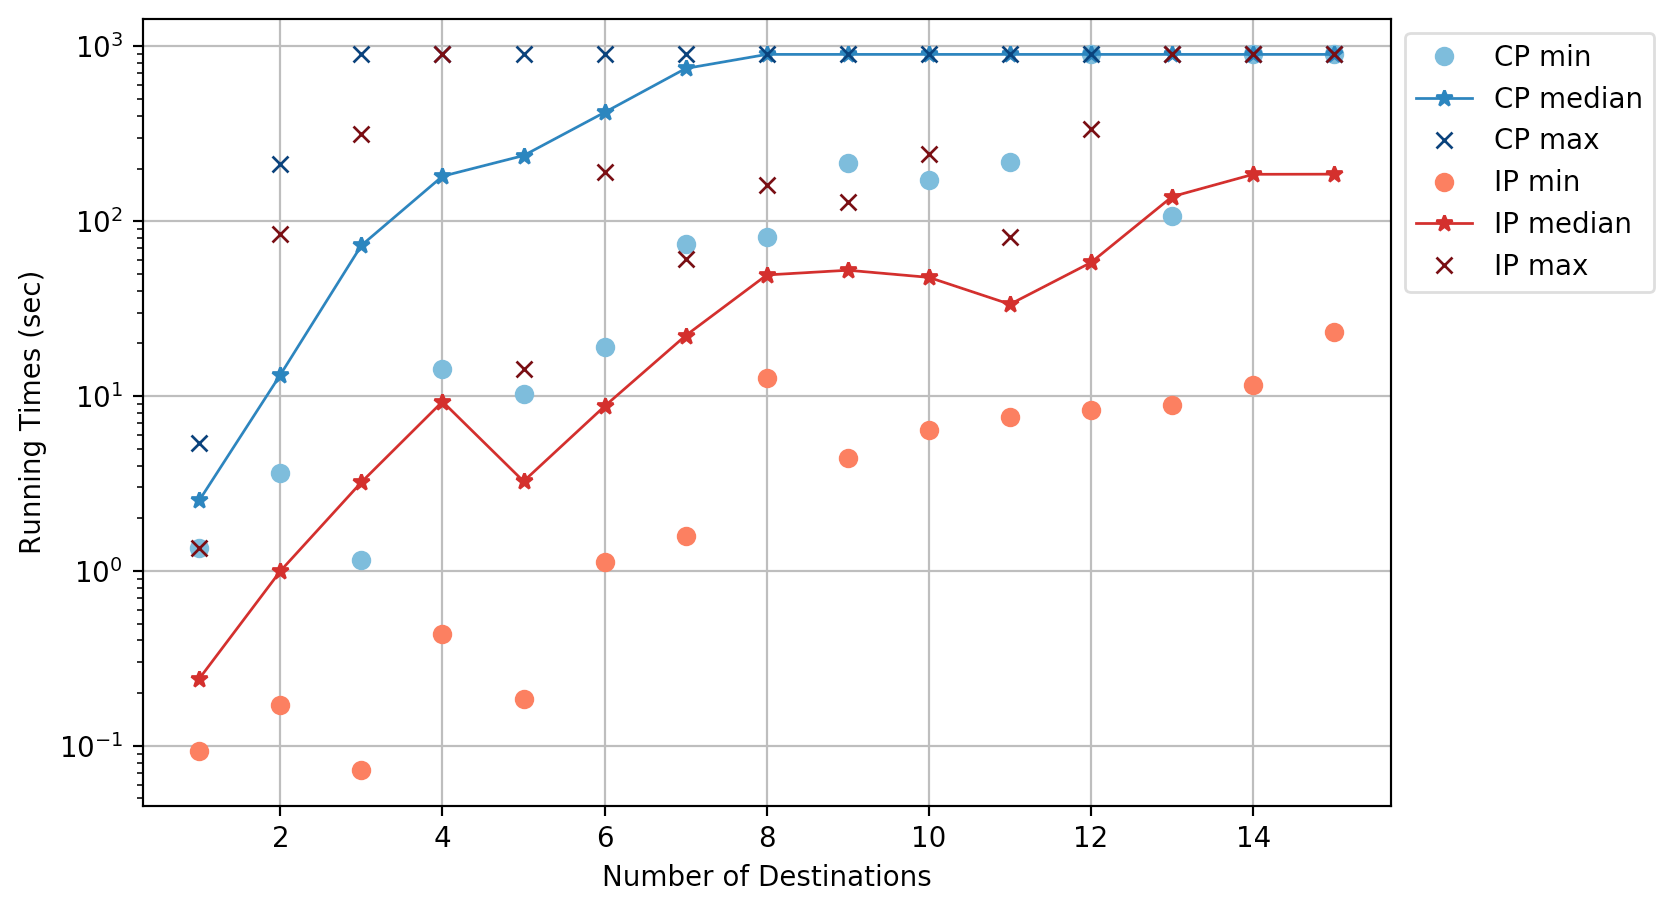
\includegraphics[width=9cm, height = 4.5cm]{cpipexperiments/d_cpip_log.png}
        \caption{$\mathcal{D}_3$}
        \label{fig:cpip_d}
    \end{subfigure}
    \begin{subfigure}[b]{0.49\textwidth}
        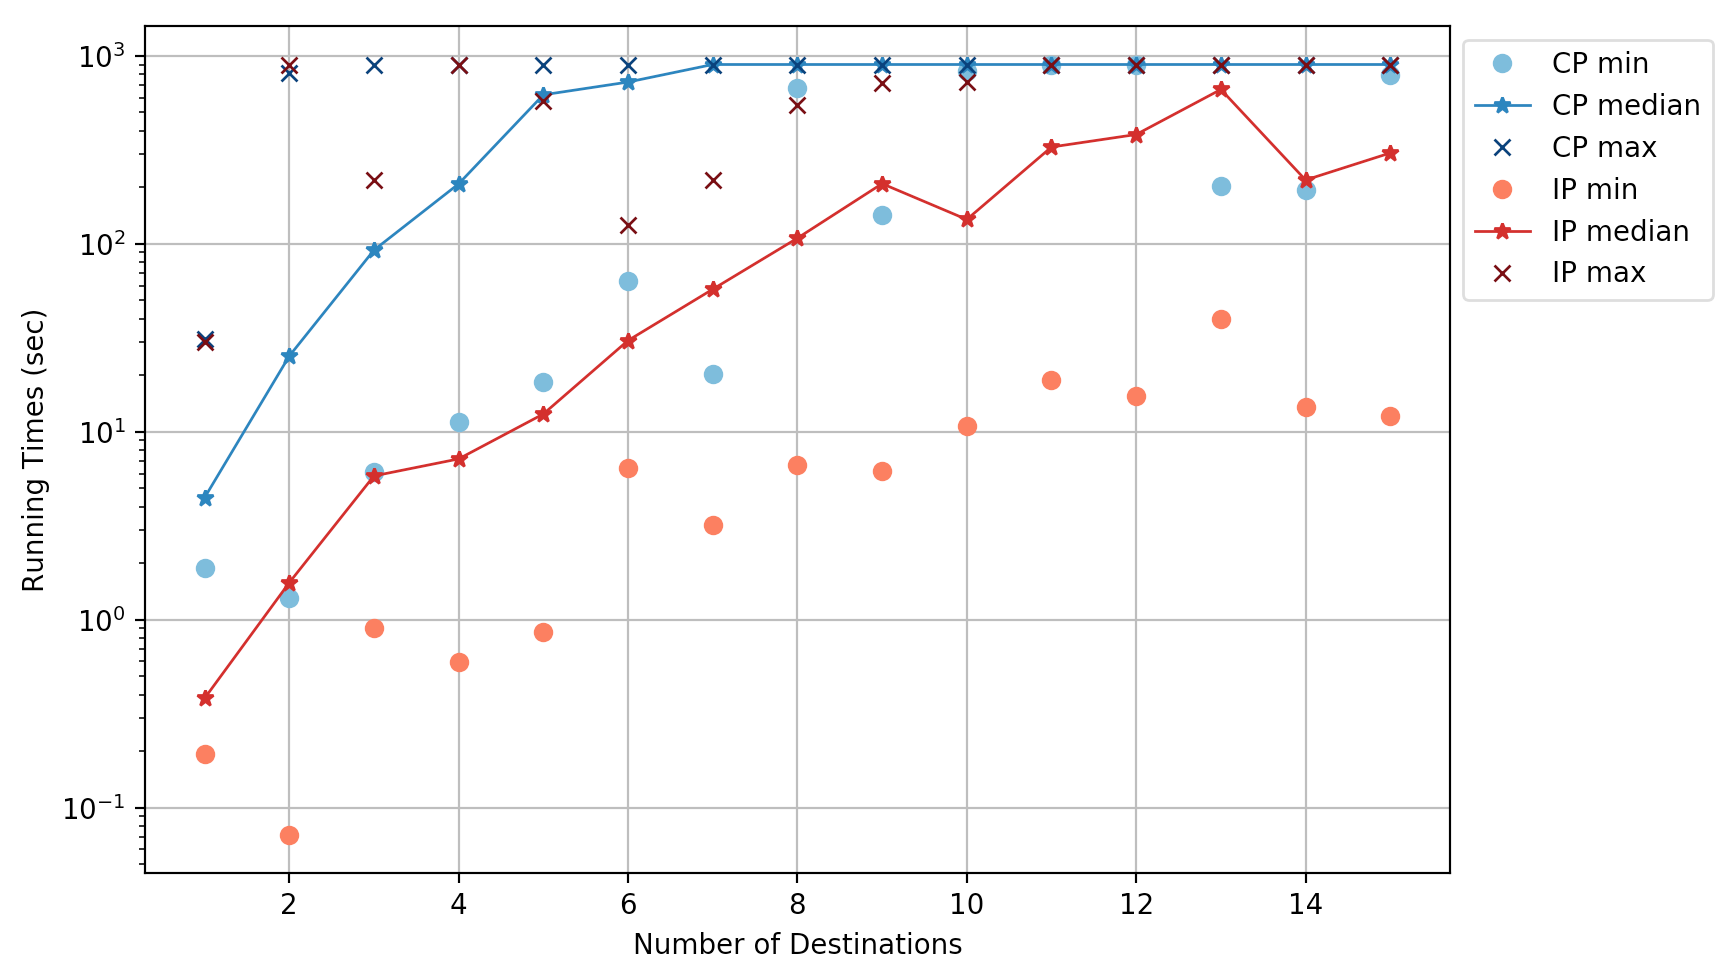
\includegraphics[width=9cm, height = 4.5cm]{cpipexperiments/d2_cpip_log.png}
        \caption{$\mathcal{D}_4$}
        \label{fig:cpip_d2}
    \end{subfigure}
    \caption{Minimum, median and maximum running time of CP (blue) and IP (red) models for each dataset.}
    \label{cpip}
\end{figure*}
%%%%%%%%%%%%%%%%%%%%%%%%
\begin{figure*}[!ht]
    \centering
    \begin{subfigure}[b]{0.49\textwidth}
        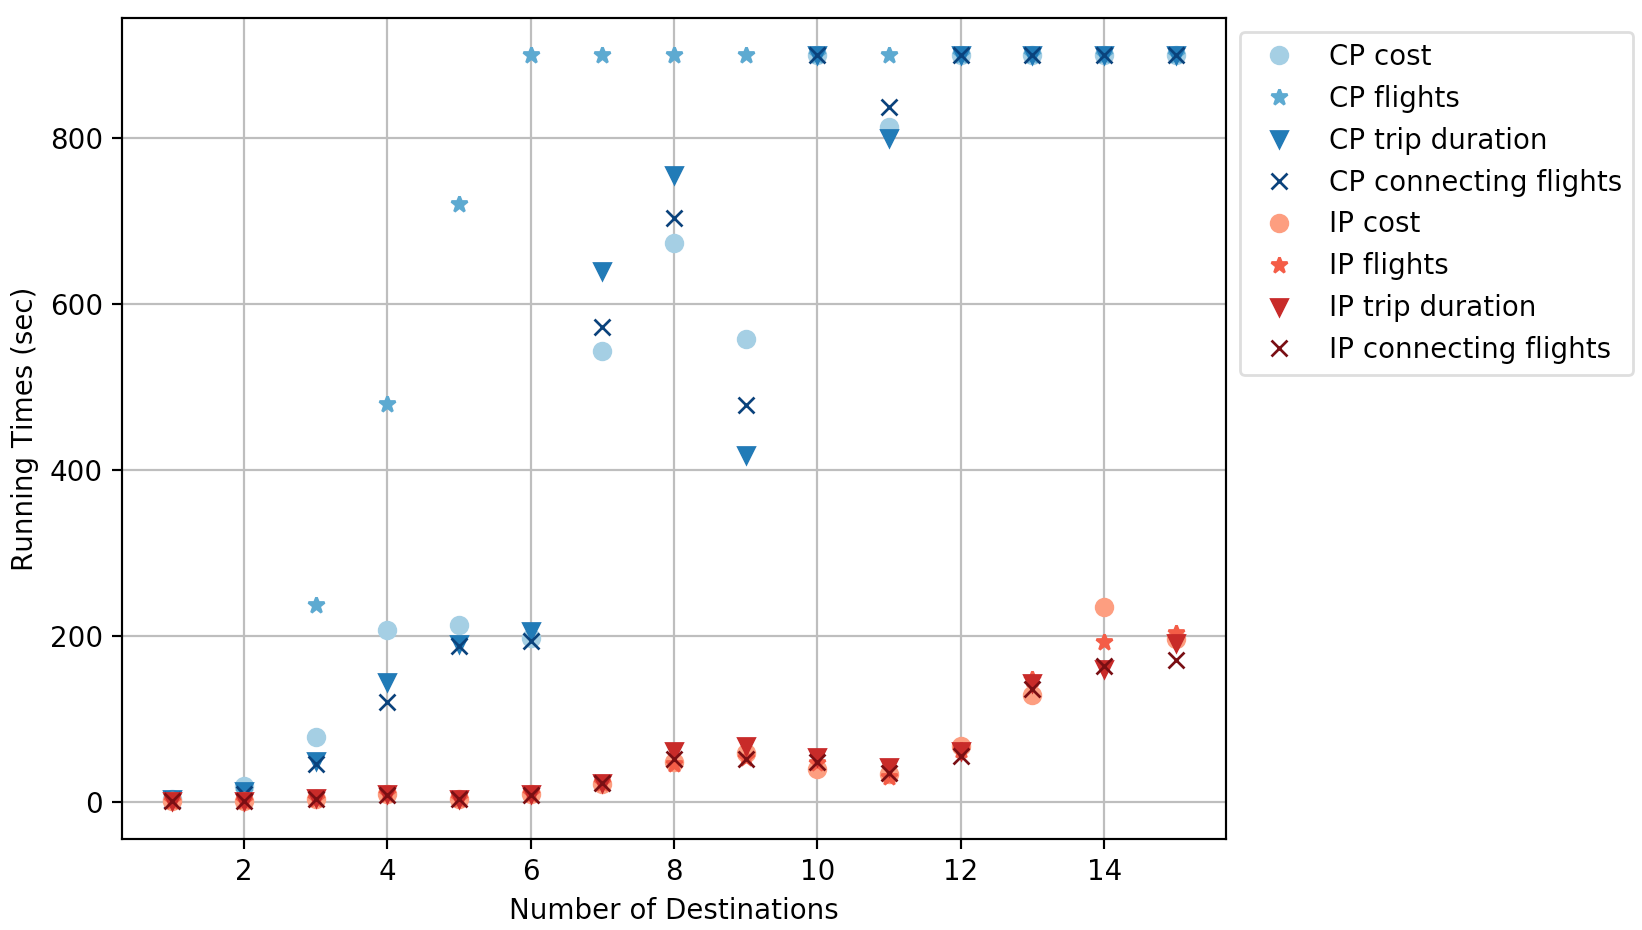
\includegraphics[width=9cm, height = 4.5cm]{cpipexperiments/cpipopt_d.png}
        \caption{$\mathcal{D}_3$}
        \label{fig:cpipopt_d}
    \end{subfigure}
    \begin{subfigure}[b]{0.49\textwidth}
        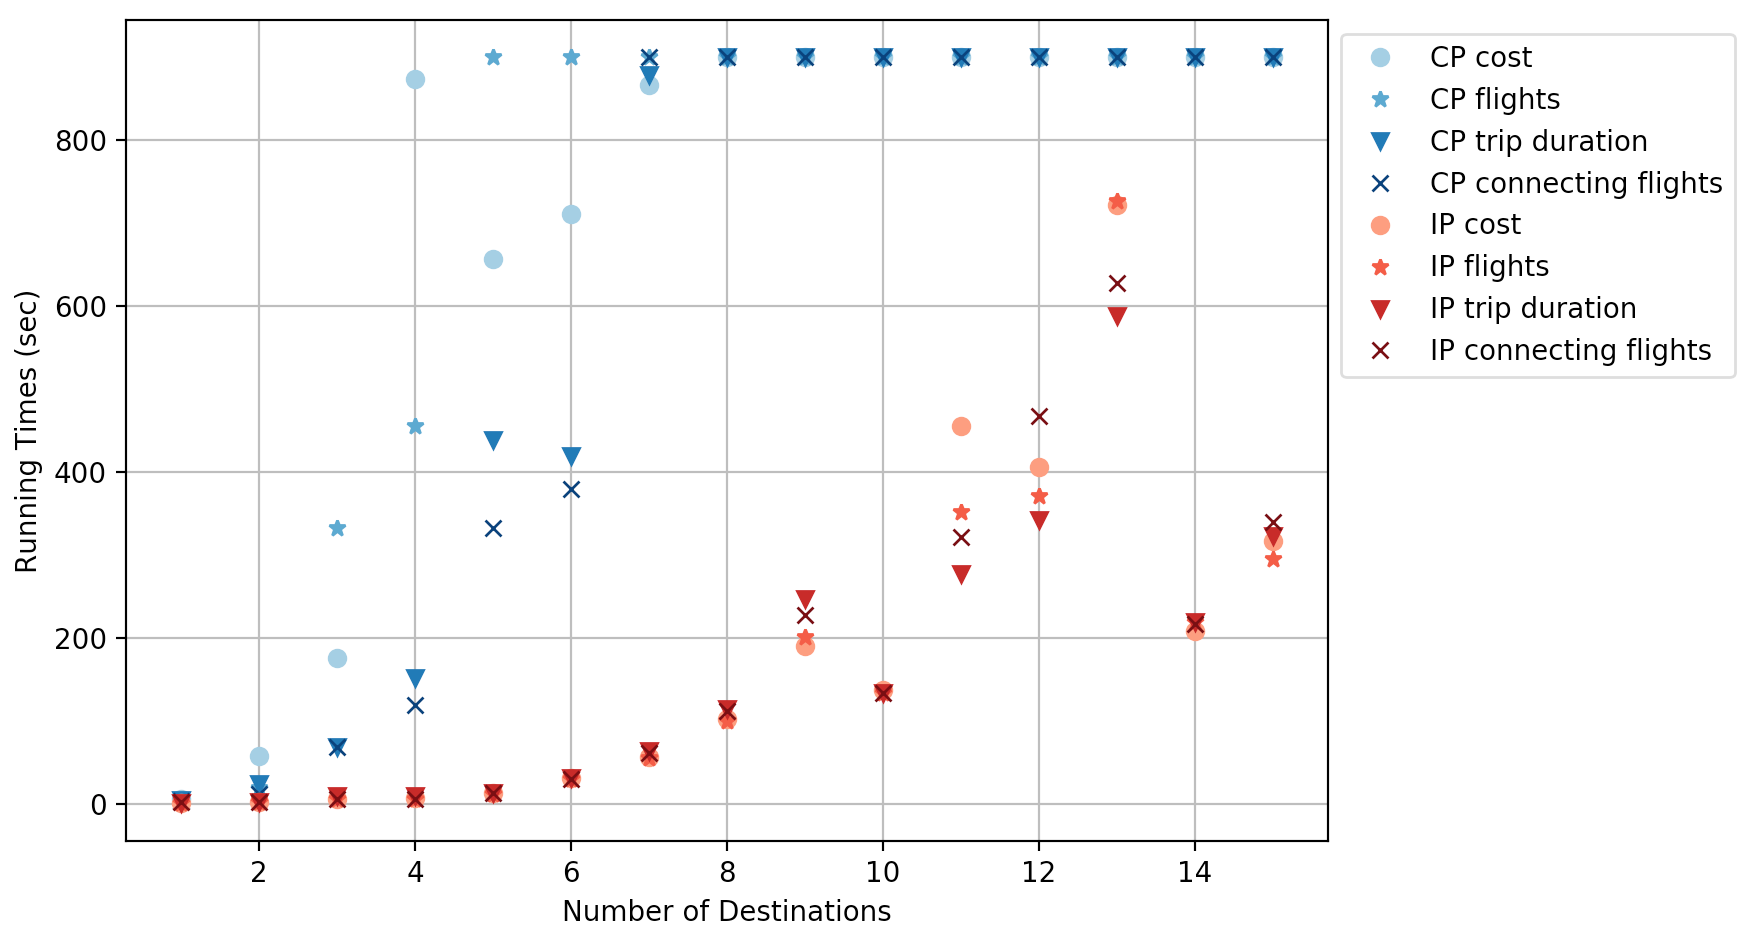
\includegraphics[width=9cm, height = 4.5cm]{cpipexperiments/cpipopt_d2.png}
        \caption{$\mathcal{D}_4$}
        \label{fig:cpipopt_d2}
    \end{subfigure}
    \caption{Median running time of each objective function for each dataset.}
    \label{cpipopt}
\end{figure*}
%%%%%%%%%%%%%%%%%%%%%%%%
\begin{figure*}[!ht]
    \centering
    \begin{subfigure}[b]{0.49\textwidth}
        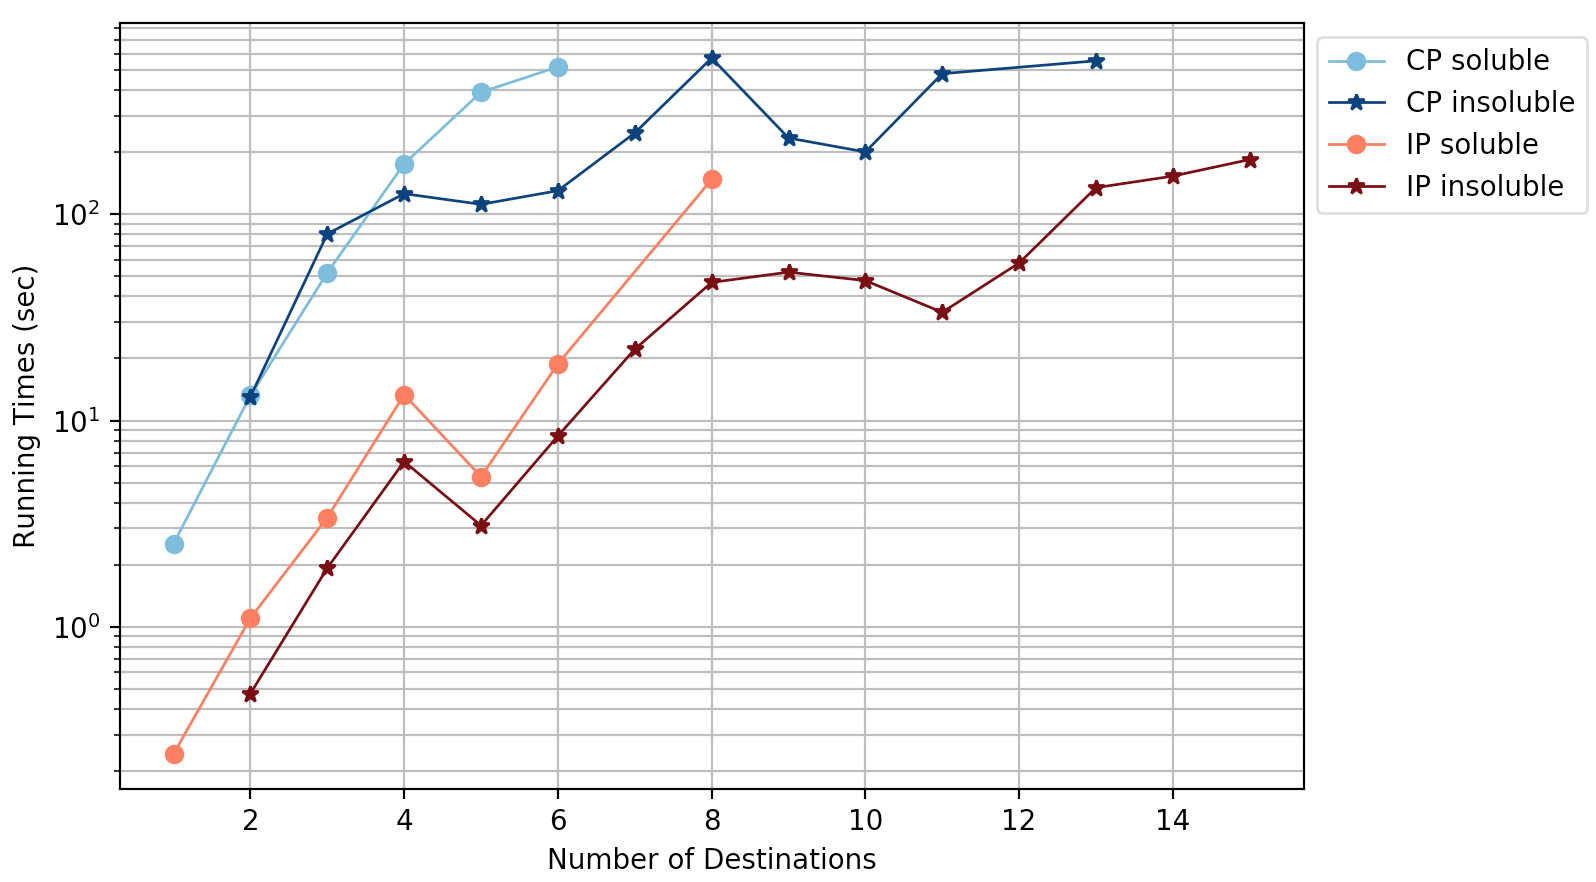
\includegraphics[width=9cm, height = 4.5cm]{cpipexperiments/cpipsatunsatnotsolved_d_log_v2.png}
        \caption{$\mathcal{D}_3$}
        \label{fig:cpipsatunsat_d}
    \end{subfigure}
    \begin{subfigure}[b]{0.49\textwidth}
        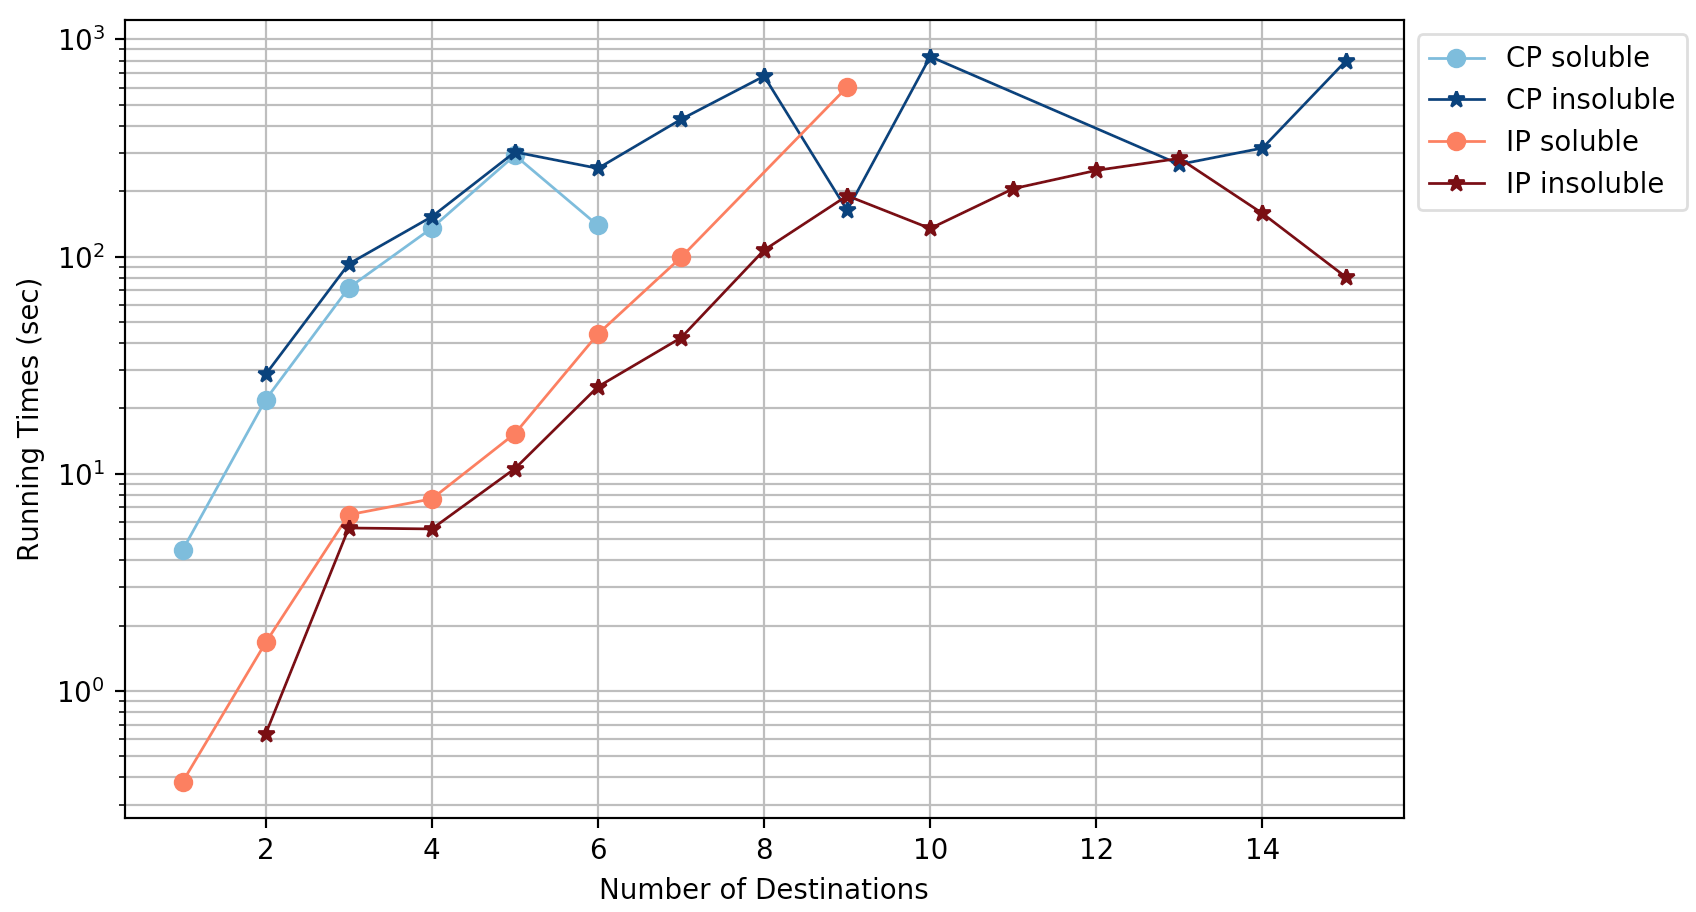
\includegraphics[width=9cm, height = 4.5cm]{cpipexperiments/cpipsatunsatnotsolved_d2_log_v2.png}
        \caption{$\mathcal{D}_4$}
        \label{fig:cpipsatunsat_d2}
    \end{subfigure}
    \caption{Median running time of IP and CP models on soluble and insoluble trials for each dataset.}
    \label{cpipsatunsat}
\end{figure*}
%%%%%%%%%%%%%%%%%%%%%%%%

\textbf{Experiment setup.} Two datasets called $\mathcal{D}_3$ and $\mathcal{D}_4$ were generated using the TP instance generator described in Section \ref{skyscannerdata} as follows. For each value of $d$ $(1 \leq d \leq 15)$, 20 TP instances were generated for each dataset, having $m$, $n$ and $T$ calculated as functions of $d$ according settings 3 and 4 for $\mathcal{D}_3$ and $\mathcal{D}_4$ respectively, as shown in Table \ref{table:testSize}. For example, in $\mathcal{D}_3$ the smallest instance has $m=20$, $n=2$, $d=1$, $T=6$, that is $(20,2,1,6)$, the largest instance has size $(300,30,15,48)$, the smallest instance in $\mathcal{D}_4$ has size $(25,2,1,6)$ and the largest instance has size $(375,30,15,48)$. This makes 300 TP instances for each dataset.

For each dataset, each instance was solved subject to each objective function in $O$ with both models. Whenever the time limit of 900 seconds was reached, the solver stopped execution, the trial is considered as not solved and no incumbent solutions are recorded.

The results are shown in Figure \ref{cpip}, Figure \ref{cpipopt} and Figure \ref{cpipsatunsat}. Each figure is discussed in the following paragraphs.

\textbf{CP and IP.} The minimum, median and maximum running time of all trials per model for every $d$ is shown in Figure \ref{fig:cpip_d} for $\mathcal{D}_3$ and in Figure \ref{fig:cpip_d2} for $\mathcal{D}_4$. For each dataset, both models show an increase in terms of the median running time with the increase of $d$, where this relationship is more evident in the CP model.

The results suggest that the IP model is better than the CP model for both $\mathcal{D}_3$ and $\mathcal{D}_4$. For example, in Figure \ref{fig:cpip_d} the minimum running time of CP for every $d \notin \{3, 13\}$ is worse than the median running time of IP. The IP model reached the time limit for $d=\{13,14,15\}$, whereas the CP model reached the time limit for every $d \notin \{1,2\}$. For $\mathcal{D}_4$, the median running time of IP is faster than the minimum running time of CP for 9 settings of $d$. Figures \ref{fig:satunsatnotsolved_cp_ip_d} - \ref{fig:dandd2solvability} further show that for both datasets the CP model reached the time limit for a much higher proportion of trials than the IP model.

% In Section \ref{sec:solvers} it was noted that both solvers are used with their default search settings, where the solvers differ in terms of employed variable selection strategy. This can be one of the reasons for the difference of the running time of the models.

\textbf{CP and IP objective functions.} For each dataset, model, objective function and value of $d$ we calculated the median running time over all trials. The results can be seen in Figure \ref{fig:cpipopt_d} for $\mathcal{D}_3$ and Figure \ref{fig:cpipopt_d2} for $\mathcal{D}_4$, where the CP results are marked in blue and the IP results are in red and the median running time over trials with objective functions $o_1$, $o_2$, $o_3$ and $o_4$ are marked by a circle, cross, triangle and asterisk respectively. For example, the median running time of the CP minimum cost objective function for $d = 4$ is 200 seconds for trials in $\mathcal{D}_3$ and about 880 seconds for trials in $\mathcal{D}_4$.

The figures show that each objective function implemented in the IP model solves trials faster than any objective function that is part of the CP model. With the increase of $d$, the superiority of IP over CP becomes more visible.

Higher variation between the running time of each objective function in the CP model for instances with $d \leq 10$ for $\mathcal{D}_3$ and $d \leq 7$ for $\mathcal{D}_4$ can be observed, where $o_1$ and $o_4$ tend to perform worse than $o_2$ and $o_3$. The reason that for high values of $d$ all objective functions are shown to perform equally well is that most trials reached the time out.
The implementation of the objective functions in the IP model have similar running times for most values of $d$, where higher variation in terms of running time can be observed only in $\mathcal{D}_4$ for high values of $d$.

\textbf{CP and IP soluble and insoluble trials.} We divided the results produced by each model into three groups: those that were found soluble, insoluble and not solved in order to compare the performance of the models for each group. The median running time of insoluble and soluble trials for every value of $d$ was calculated and all not solved trials were discarded, since their running time is always 900 seconds. Figure \ref{cpipsatunsat} shows the results, where Figure \ref{fig:cpipsatunsat_d} is for $\mathcal{D}_3$ and Figure \ref{fig:cpipsatunsat_d2} for $\mathcal{D}_4$. We note that the numbers of soluble, insoluble and not solved trials for each dataset differ across the two models. Their proportion for each value of $d$ for each model and for each dataset are shown in Figure \ref{fig:satunsatnotsolved_cp_ip_d} and Figure \ref{fig:satunsatnotsolved_cp_ip_d2}.

%% left figure
Figure \ref{fig:cpipsatunsat_d} shows that the IP model has faster median running time than the CP model for both soluble and insoluble trials. An increase of the median running time with the increase of $d$ is observed for both groups of trials for each model, where this relationship is more evident in the CP model: for $d = 8$, the CP model solved 0 soluble trials and for $d=\{14, 15\}$, CP reached the time limit for all trials.

%% right figure
Figure \ref{fig:cpipsatunsat_d2} shows similar results. The IP model is faster than the CP model for every $d \notin \{9,13\}$, where for $d = 13$ insoluble CP and IP trials have equal median running time and for $d=9$, the CP model is slightly quicker.

%% both figures
For $d = 0$, both models encountered 0 insoluble trials in both datasets and for high values of $d$ none of the models found soluble trials. Figure \ref{fig:satunsatnotsolved_ip_d} and Figure \ref{fig:satunsatnotsolved_ip_d2} show the reason: increasing $d$ decreases the proportion of soluble instances for both datasets. This suggests that the chosen relationship between $d$ and $m$, $n$ and $T$ in $\mathcal{D}_3$ and $\mathcal{D}_4$ shown in Table \ref{table:testSize} is not successful in creating soluble instances for high values of $d$.

%% comparison of sat/unsat for the same model
The IP model finds proving insolubility easier than finding an optimal solution: for every value of $d$ for both $\mathcal{D}_3$ and $\mathcal{D}_4$, insoluble trials were solved quicker than soluble trials (Figure \ref{cpipsatunsat}). A possible reason for obtaining these results is that once a trial is found to be insoluble, the solver can terminate execution, whereas finding a solution to a trial does not immediately guarantee its optimality.

\subsection{Multiobjective Optimisation}
\label{experiments:multiobjective}

This section evaluates the performance of the CP and IP multiobjective optimisation implementations and uses notation previously introduced in Section \ref{multiobjOpt}.

%%%%%%%%%%%%%%%%%%%%%%%%
\begin{figure*}[!ht]
    \centering
    \begin{subfigure}[b]{0.24\textwidth}
        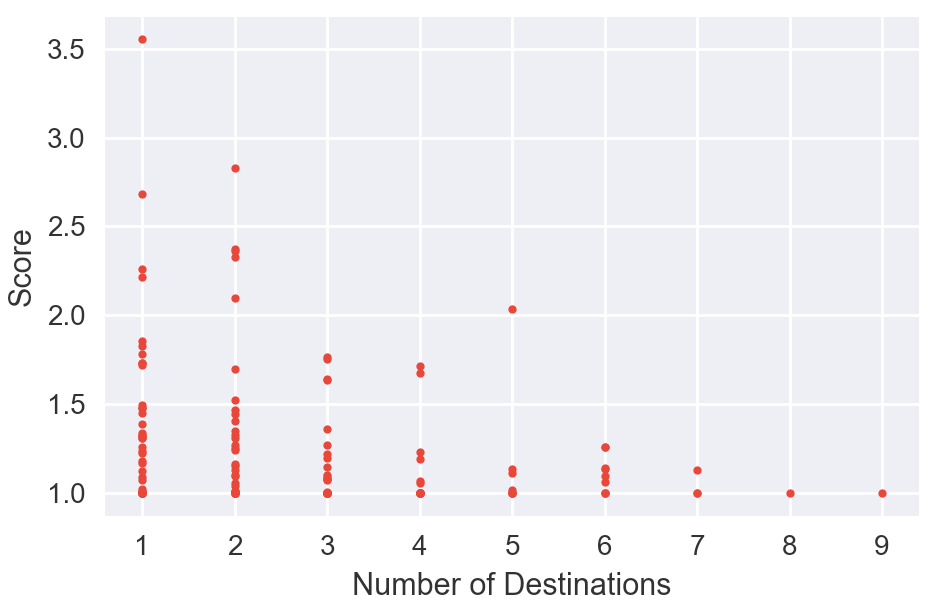
\includegraphics[width=\textwidth, height=3.5cm]{cost_ip.png}
        \caption{min cost ($o_1$)}
        \label{costip}
    \end{subfigure}
    \begin{subfigure}[b]{0.24\textwidth}
        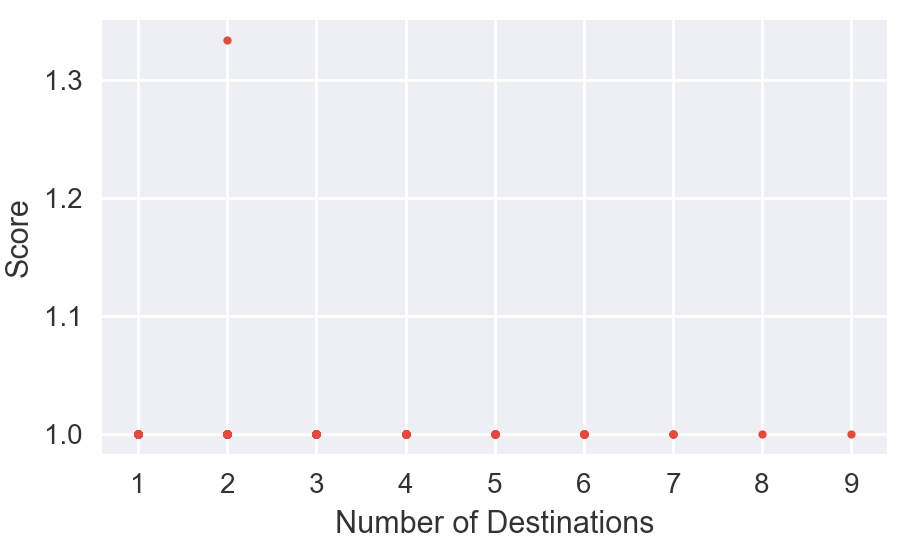
\includegraphics[width=\textwidth, height=3.5cm]{connair_ip.png}
        \caption{min connecting airports ($o_2$)}
        \label{airportsip}
    \end{subfigure}
    \begin{subfigure}[b]{0.24\textwidth}
        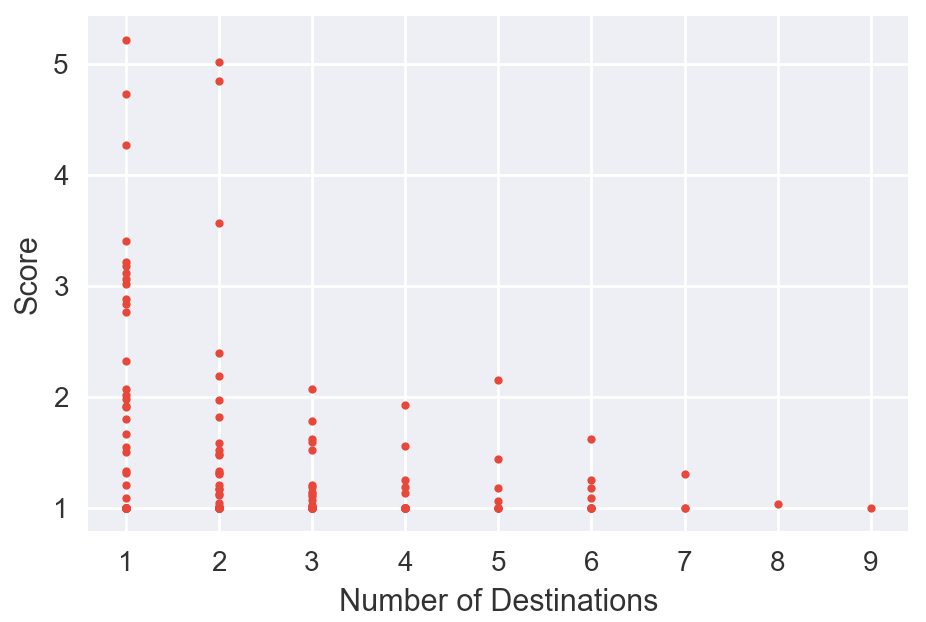
\includegraphics[width=\textwidth, height=3.5cm]{trip_ip.png}
        \caption{min trip duration ($o_3$)}
        \label{tripip}
    \end{subfigure}
    \begin{subfigure}[b]{0.24\textwidth}
        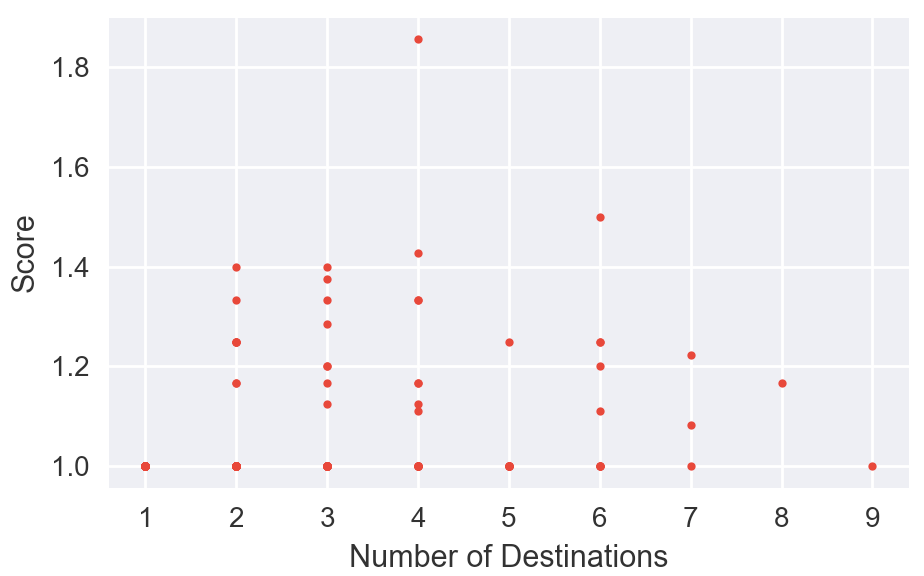
\includegraphics[width=\textwidth, height=3.5cm]{flights_ip.png}
        \caption{min number of flights ($o_4$)}
        \label{flightsip}
    \end{subfigure}
    \caption{The scores of all optimal solutions returned by the IP model, relative to each objective and grouped by $d$.}
    \label{fig:ipmultiobj}
\end{figure*}
%%%%%%%%%%%%%%%%%%%%%%%%
\begin{figure*}[!ht]
    \centering
    \begin{subfigure}[b]{0.24\textwidth}
        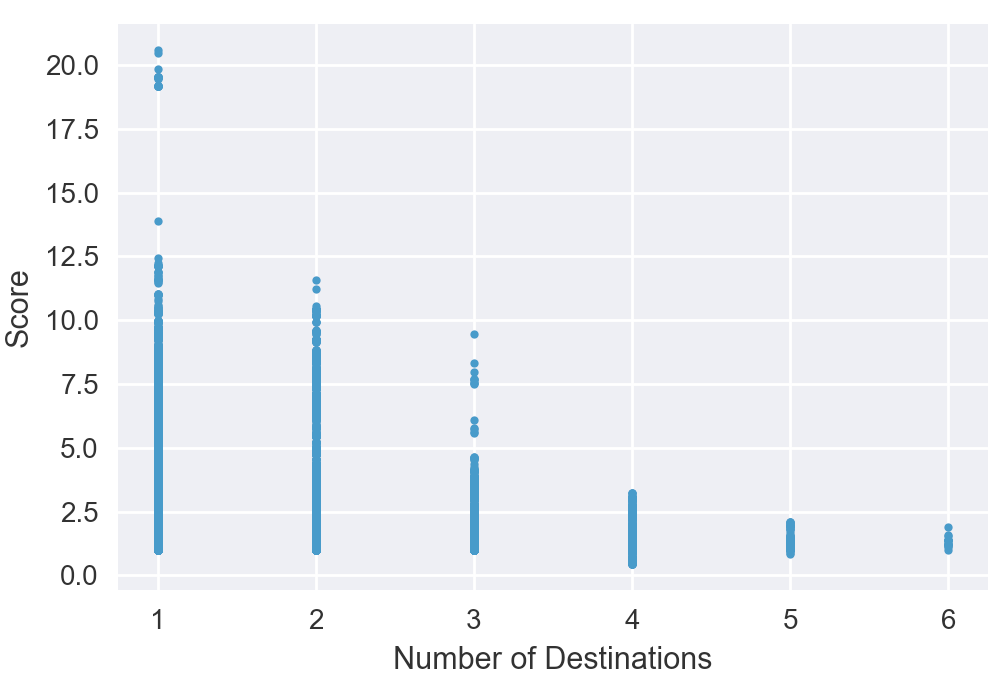
\includegraphics[width=\textwidth, height=3.5cm]{cost_cp.png}
        \caption{min cost ($o_1$)}
        \label{costcp}
    \end{subfigure}
    \begin{subfigure}[b]{0.24\textwidth}
        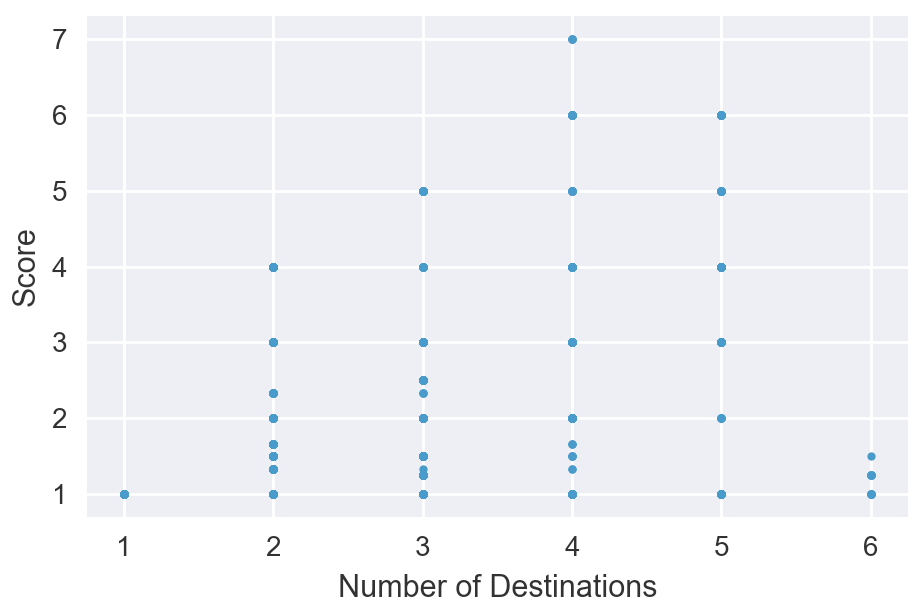
\includegraphics[width=\textwidth, height=3.5cm]{connair_cp.png}
        \caption{min connecting airports ($o_2$)}
        \label{airportscp}
    \end{subfigure}
    \begin{subfigure}[b]{0.24\textwidth}
        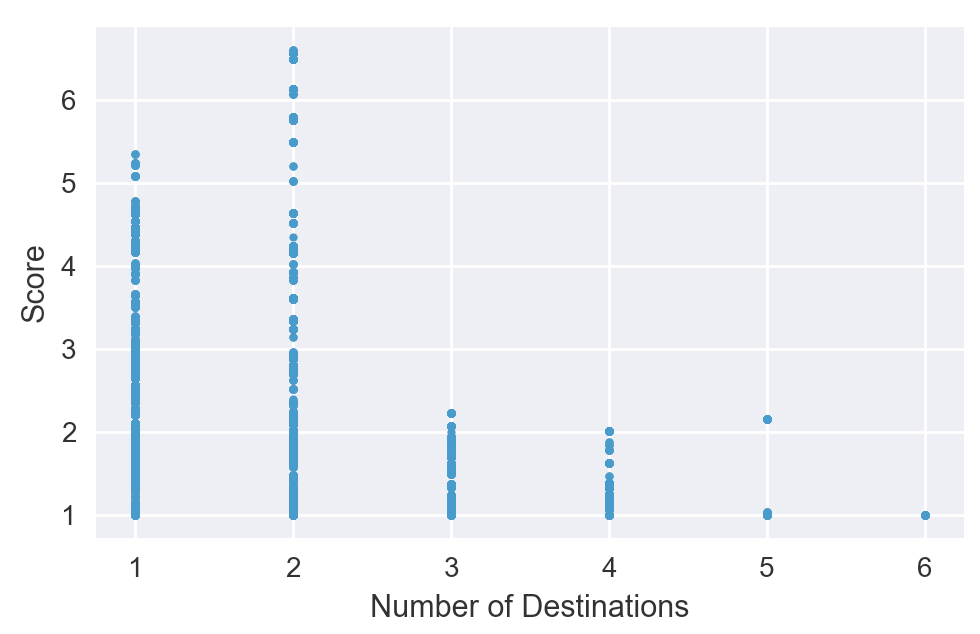
\includegraphics[width=\textwidth, height=3.5cm]{trip_cp.png}
        \caption{min trip duration ($o_3$)}
        \label{tripcp}
    \end{subfigure}
    \begin{subfigure}[b]{0.24\textwidth}
        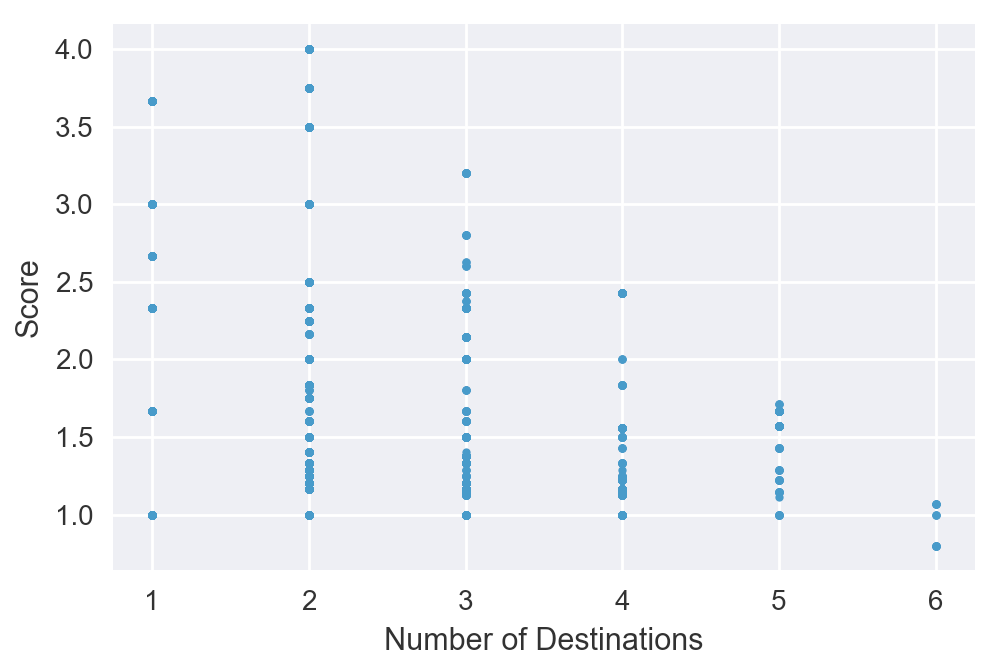
\includegraphics[width=\textwidth, height=3.5cm]{flights_cp.png}
        \caption{min number of flights ($o_4$)}
        \label{flightscp}
    \end{subfigure}
    \caption{The scores of all optimal solutions returned by the CP model, relative to each objective and grouped by $d$.}
    \label{fig:cpmultiobj}
\end{figure*}
%%%%%%%%%%%%%%%%%%%%%%%%

Let $\omega(S,o_{r})$ be the \textit{score} of a solution $S \in \mathcal{F}(\pi)$ relative to objective $o_r \in O$, where $\omega(S,o_{r})$ is calculated as follows:
\vspace{-1mm}
\begin{equation}
\label{eq:score}
\omega(S,o_{r}) = \frac{g_{r}(S) + 1}{S(\pi,o_r)^\ast + 1} \textrm{,}
\end{equation}
where the addition of 1 to both the numerator and the denominator is done in order to avoid division by 0 or obtaining score equal to 0.
Whenever $g_{r}(S) = S(\pi, o_r)^\ast$, then $\omega(S,o_{r}) = 1$ and this means that solution $S$ is an optimum with respect to $o_r$. Note that $\omega(S,o_{r}) \geq 1$, since $o_r$ is a minimisation objective. Therefore, solutions with high score have value far from the optimum relative to the measured objective. Calculating scores of solutions is used as a normalisation technique: the measure of performance over all objectives is adjusted to a common scale, so that comparison between them is possible.

Let $\mathcal{D}_5$ be the union of all TP instances in datasets $\mathcal{D}_3$ and $\mathcal{D}_4$, discussed in the previous section, that have known optimal solutions for each objective function by both models. For every $\pi \in \mathcal{D}_5$, we solved $tr(\pi,O)$ with both models with $O$ as defined in the beginning of Section \ref{evaluation}. The CP model returned the Pareto frontier of $tr(\pi,O)$, which in general comprises multiple solutions for every trial, whereas the IP model returned one solution for each trial. The weight $w_r$ of each objective $o_r$ is equal to $\frac{1}{4}$ (that is, the four objectives have equal weight). For each objective in $O$, the score of every solution returned by each model was calculated. The obtained results from each trial and objective, grouped by $d$, are shown in Figure \ref{fig:ipmultiobj} for the IP model and in Figure \ref{fig:cpmultiobj} for the CP model, where Figure \ref{fig:cpmultiobj} shows all members of the Pareto frontier for each trial.

The scores of all trials relative to $o_1$, $o_3$ and $o_4$ tend to decrease with the increase of $d$ for both models (Figure \ref{fig:ipmultiobj} and Figure \ref{fig:cpmultiobj}). Possible explanation of this result could be the following. It was observed in the previous section that with the increase of $d$ the number of soluble trials decreases and the number of trials that reach the time limit increases. This suggests that as $d$ increases, the number of solutions returned by each model is smaller and it is produced after solving only ``easier'' trials (that is, trials that did not reach the time limit), which causes having less variation and lower scores for higher values of $d$. However, this hypothesis does not explain the results for $o_2$ (Figures \ref{airportsip} and \ref{airportscp}).

The highest scores were obtained for the solutions returned by the CP model relative to $o_1$ (Figure \ref{costcp}) and the lowest scores were obtained for the solutions returned by the IP model relative to $o_2$ (Figure \ref{airportsip}). For every objective, the scores of the solutions obtained from the IP model are lower than the scores of the solutions returned by the CP model. This suggests that Pareto optimality is much weaker than optimality with respect to the scalarisation objective.

\subsection{Empirical study of the IP model}
\label{experiments:ipmodel}
The experiments in this section investigate the influence of the number of flights $m$, airports $n$, destinations $d$ and holiday time $T$ on the running time of the IP model and the solubility of the TP instances.

Similarly to the experiments in the previous section, each instance was solved subject to each of the 4 implemented objective functions, that is 4 trials per instance. For each trial, a time limit of 15 minutes was imposed on the solver. Whenever the time limit is reached, the solver returns the incumbent solution, if found, and stops execution.

The results from each experiment are represented by three plots, where each left-most plot (Figure \ref{fig:exp1all}, Figure \ref{fig:exp2all}, Figure \ref{fig:exp3all} and Figure \ref{fig:exp4all}) is generated as follows. For each varied setting of either $m$, $n$, $d$ or $T$, the running times of all trials are sorted from least to greatest, divided into four quartiles and plotted using a \textit{box and whiskers} plot as follows. A rectangle represents all running times within the second and the third quartile. The horizontal orange bar across the rectangle is the median and it divides the data into two parts. The vertical black lines connected to the rectangle from below and from above are referred to as \textit{upper whisker} and \textit{lower whisker} respectively. They represent running times in the fourth and the first quartile respectively. The black horizontal bar at the end of each whiskers marks the lowest or highest running time, excluding outliers. \textit{Outliers} are running times that are at least 1.5 times lower than the range of values in the lower whisker or 1.5 times higher than the data range in the upper whiskers. Outliers are represented by green diamonds.

For each experiment, the middle plot (Figure \ref{fig:exp1sat}, Figure \ref{fig:exp2sat}, Figure \ref{fig:exp3sat} and Figure \ref{fig:exp4sat}) divides all solved trials into soluble and insoluble and shows the minimum, median and maximum running time of the IP solver for each group and each varied parameter.

For each experiment, the right-most plot (Figure \ref{fig:varymsat}, Figure \ref{fig:varynsat}, Figure \ref{fig:varydsat} and Figure \ref{fig:varytsat}) shows the percentage of solved (red for soluble and blue for insoluble instances) and not solved (green) trials for each varied parameter.

\textbf{Experiment 1.} In the first experiment, we increased the number of flights $m$ while maintaining constant numbers of airports $n$, destinations $d$ and holiday time $T$. For values of $m$ $(100 \leq m \leq 500)$ in increments of 40, 10 TP instances were generated with $n=11$, $d=6$ and $T=14$.

Figure \ref{experiment1} shows the obtained results.
Figure \ref{fig:exp1all} suggests that the running time rapidly increases with the increase of $m$. Most trials with $m \leq 220$ are solved within 200 seconds. However, for values of $m \geq 340$ most of the trials reached the time limit: the running time of all quartiles is 15 minutes, where for $m=460$, all trials reached the time limit.

A slight decrease of the running time for trials with $m=500$ can be seen, showing that for the chosen values of $n$, $d$ and $T$, the instances with $m=460$ take most time to solve. The region where problems change from being soluble to insoluble and their difficulty increases dramatically is referred to as \textit{phase transition}. Figure \ref{experiment1} shows a possible existence of a phase transition for Experiment 1, occurring at $m=460$. Effective methods to predict problem difficulty using phase transitions have been developed \cite{Prosser1996,Cheeseman:1991}.

Figure \ref{fig:exp1sat} shows that the IP model is faster at solving insoluble trials than soluble trials. The same result was observed in the experiments described in Section \ref{experiments:cpvsip}.

Figure \ref{fig:varymsat} shows an increase in the proportion of not solved trials as $m$ increases, where for $m=460$ all trials were not solved. For values of $m \leq 220$ an increase of the proportion of soluble trials can be observed with the increase of $m$, whereas for $m > 220$ there is lower number of soluble trials. These results can be explained as follows. Experiments show that the IP model is faster when run on insoluble trials. Therefore, soluble trials are expected to hit the time limit more often than insoluble trials, provided that the trials have the same size. Since there is a trend of increase in soluble trials for $m \leq 220$, we believe that the number of green trials that are soluble is higher than the number of green trials that are insoluble.

\textbf{Experiment 2.} In the second experiment, we increased $n$ while maintaining constant numbers of $m$, $d$ and $T$. For each $n$ $(7 \leq n \leq 20)$, 10 TP instances were generated, with $m = 150$, $d=6$ and $T=14$.

Figure \ref{experiment2} shows the obtained results: in Figure \ref{fig:exp2all} it can be seen that only five trials reached the time limit and most of the trials were solved within 200 seconds time. A slight decrease of the running time with the increase of $n$ can be observed. Figure \ref{fig:exp1sat} confirms previous observations that the IP model runs faster on insoluble trials.

Figure \ref{fig:varynsat} shows that increasing $n$ results in an increase of the proportion of insoluble trials, where for $17 \leq n \leq 20$ all trials are insoluble. This is due to the TP instance generator: adding more airports to an instance while maintaining $m$ constant reduces the proportion of flights that visit destinations. The SCC test does not account for flight dates and therefore it is insufficient for filtering instances with high number of airports, compared to flights. %In order to obtain higher number of soluble instances for high values of $n$, a stronger filtering test is needed.

\textbf{Experiment 3.} In the third experiment, we increased $d$ while maintaining constant numbers of $m$, $n$ and $T$. For each $d$ $(1 \leq d \leq 10)$, 10 TP instances were generated, containing $m = 150$, $n=11$ and $T=14$.

The results in Figure \ref{experiment3} show that there is no particular relation between the running time and the value of $d$: the median for each $d$ is about 50 seconds and almost all trials were solved for less than 200 seconds.

Similarly to Figure \ref{fig:varynsat}, Figure \ref{fig:varydsat} suggests that as $d$ is increased, a larger proportion of the generated TP instances are insoluble most likely for similar reasons. 

\textbf{Experiment 4.} In the fourth experiment, we increased $T$ while maintaining constant numbers of $m$, $n$ and $d$. For each $T$ $(7 \leq T \leq 20)$ in increments of 2, 10 TP instances were generated, containing $m = 150$, $n=11$ and $d=6$.

The results can be seen in Figure \ref{experiment4}, where Figure \ref{fig:exp4all} shows that most trials were solved in under 200 seconds time and that no particular relation between the value of $T$ and the running time can be observed. Figure \ref{fig:exp4sat} confirms the previously noted observation that the IP model is better at solving insoluble instances. Figure \ref{fig:varytsat} suggests that there is no particular relation between the value of $T$ and the instance solubility, where the reason for having only insoluble trials for $T = \{7,17\}$ is unknown.

%%%%%%%%%%%%%%%%%%%%%%%%
\begin{figure*}[!ht]
    \centering
    \begin{subfigure}[b]{0.30\textwidth}
        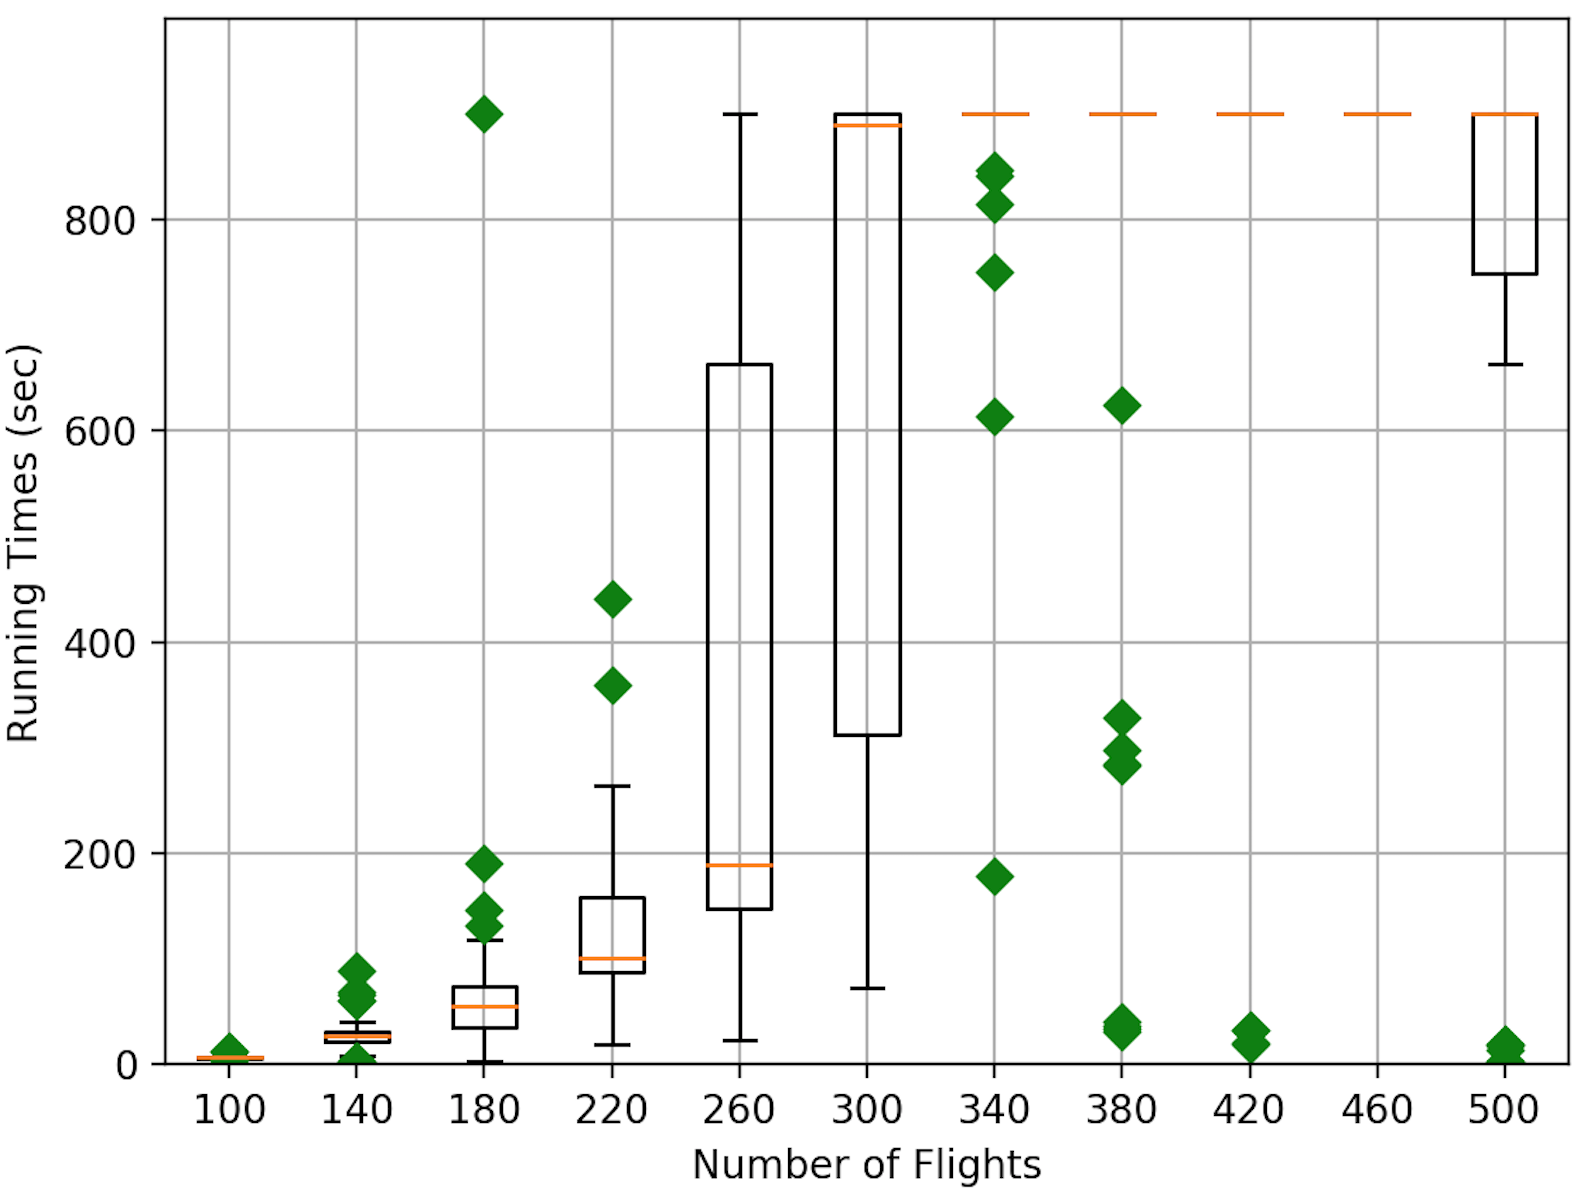
\includegraphics[width=\textwidth, height=4cm]{images/experiments/varym/varyM.png}
        \caption{all trials}
        \label{fig:exp1all}
    \end{subfigure}
    \begin{subfigure}[b]{0.36\textwidth}
        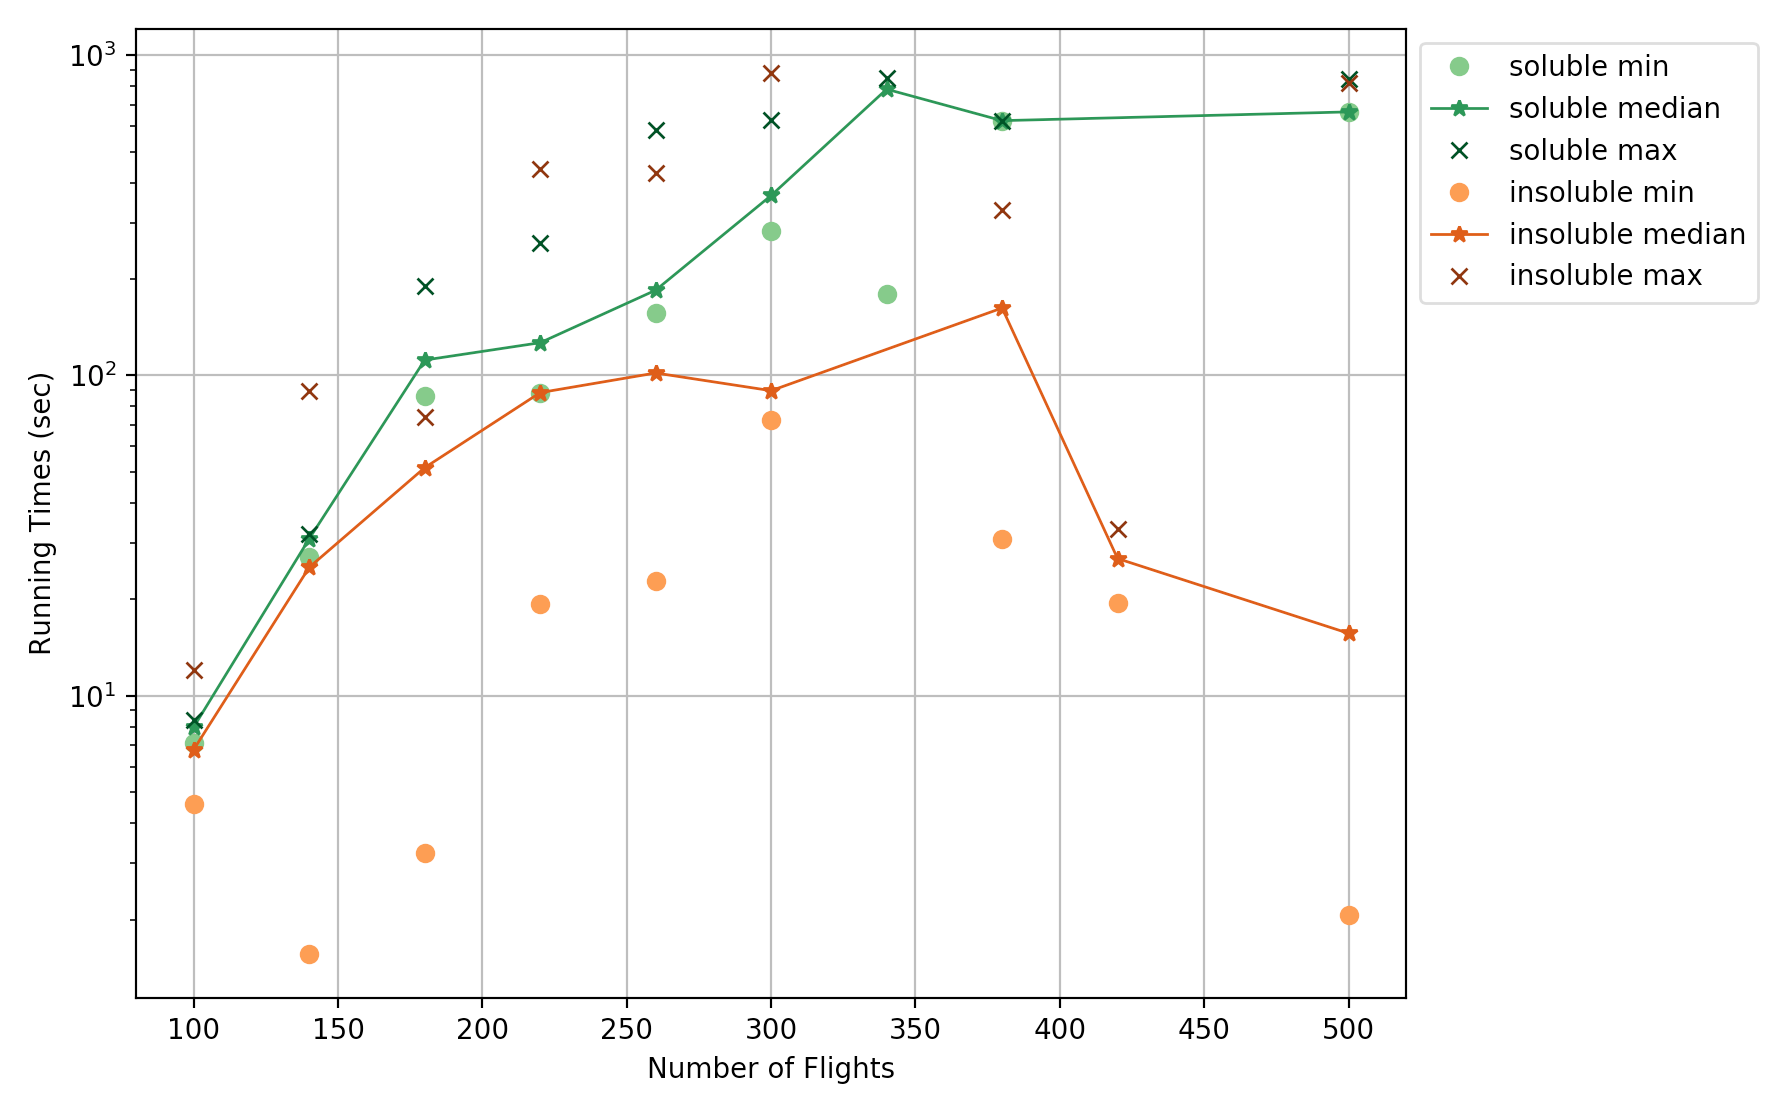
\includegraphics[width=\textwidth, height=4cm]{images/experiments/varym/satunsat_m.png}
        \caption{soluble vs insoluble trials}
        \label{fig:exp1sat}
    \end{subfigure}
    \begin{subfigure}[b]{0.32\textwidth}
        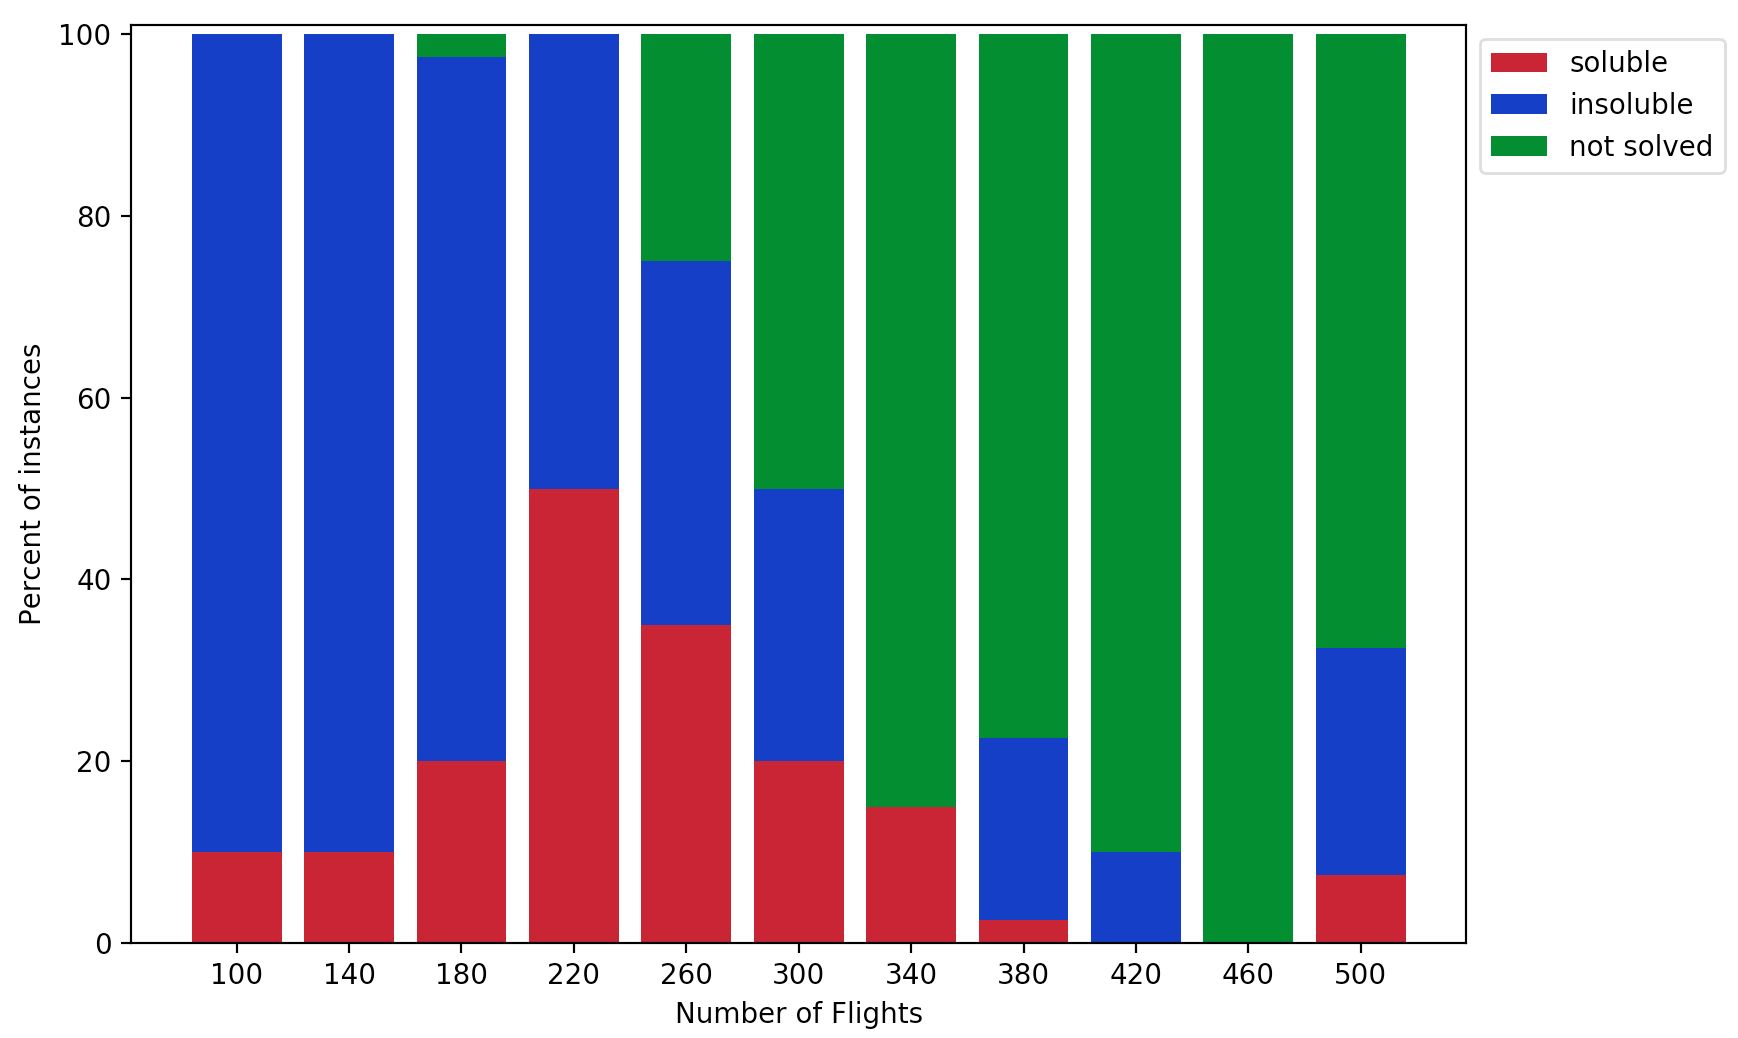
\includegraphics[width=\textwidth, height=4cm]{images/experiments/varym/varyMsat.png}
        \caption{solubility of trials}
        \label{fig:varymsat}
    \end{subfigure}
    \caption{Experiment 1}
    \label{experiment1}
\end{figure*}
\vspace{-1mm}
%%%%%%%%%%%%%%%%%%%%%%%%
\begin{figure*}[!ht]
    \centering
    \begin{subfigure}[b]{0.30\textwidth}
        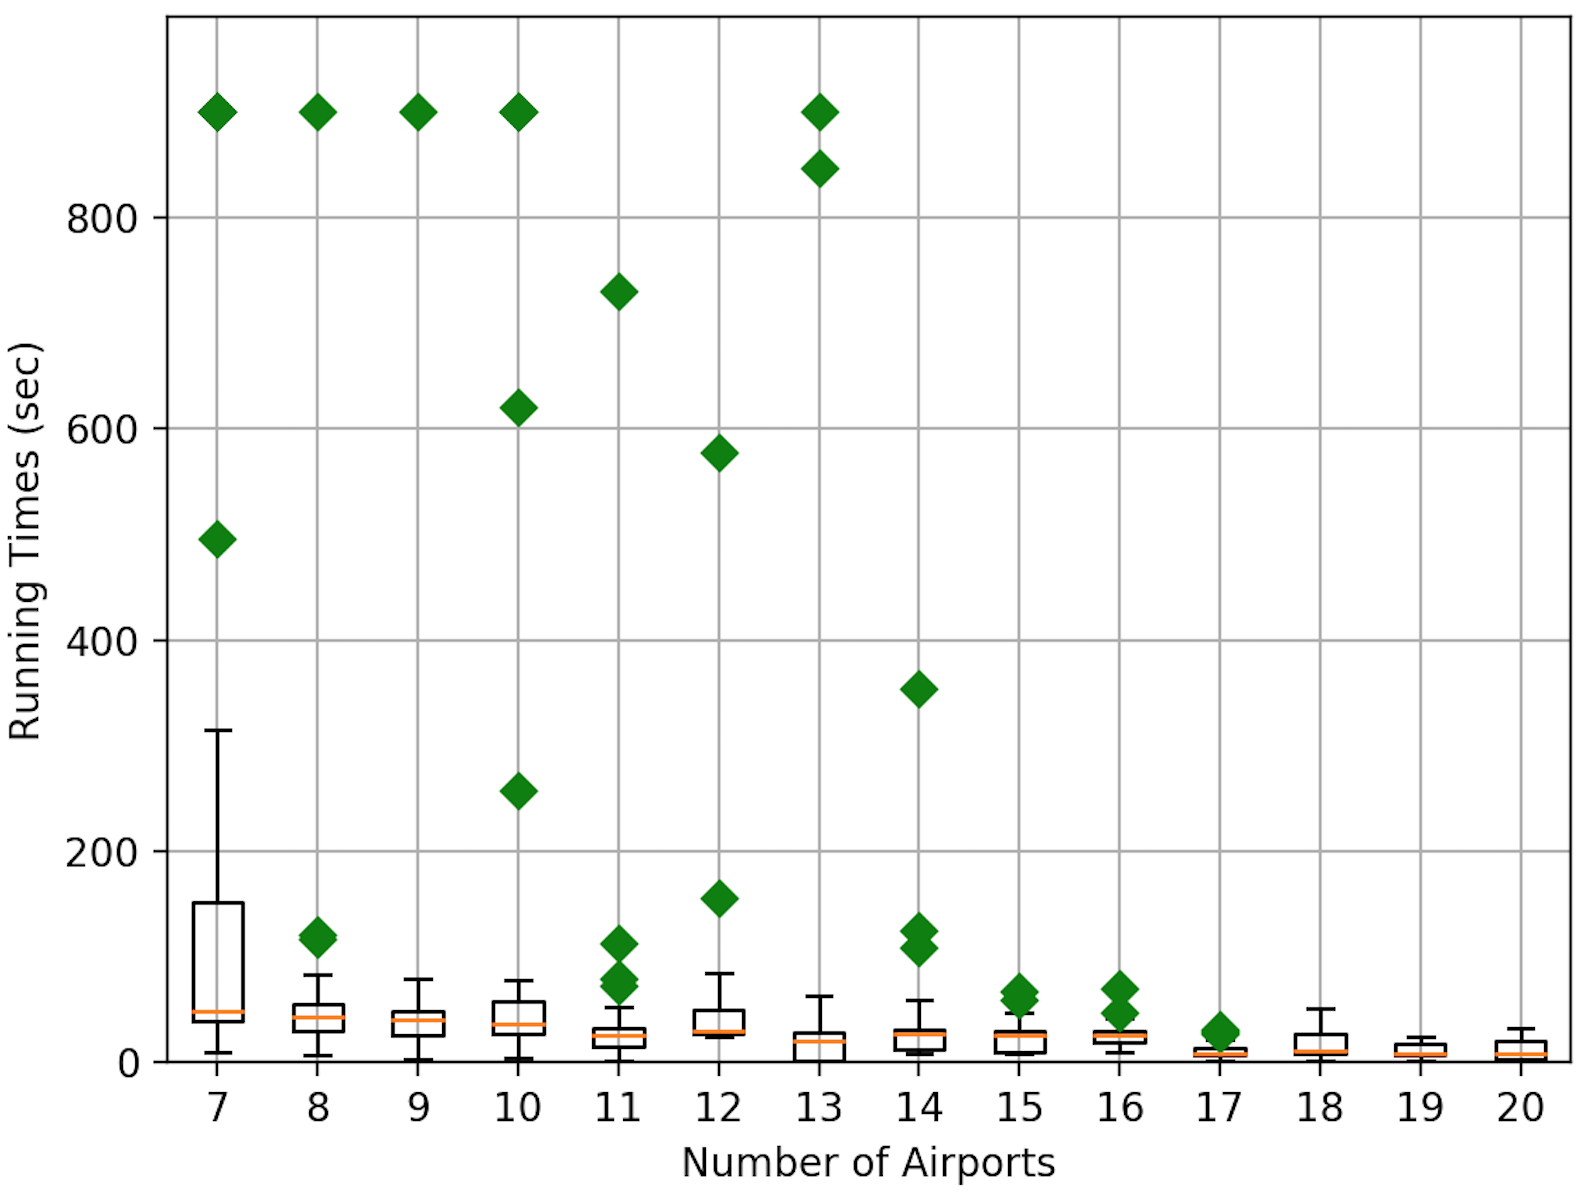
\includegraphics[width=\textwidth, height=4cm]{images/experiments/varyn/varyN.png}
        \caption{all trials}
        \label{fig:exp2all}
    \end{subfigure}
    \begin{subfigure}[b]{0.36\textwidth}
        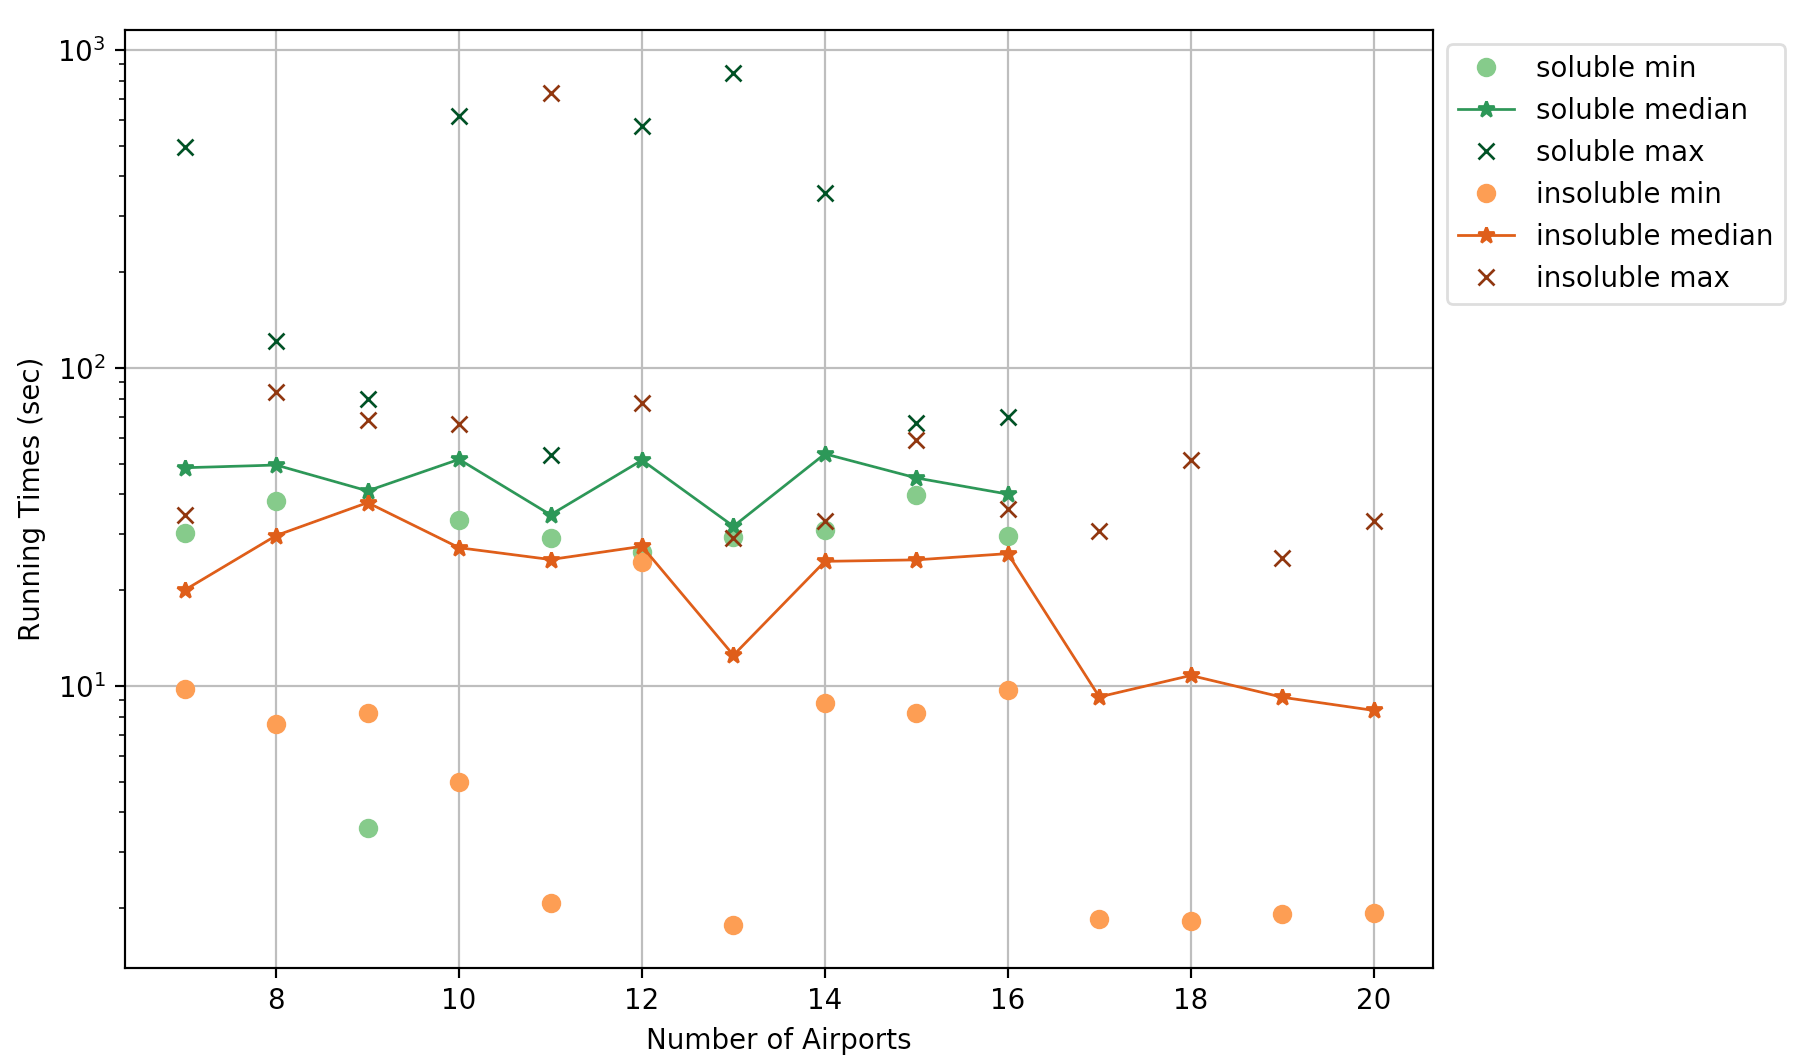
\includegraphics[width=\textwidth, height=4cm]{images/experiments/varyn/satunsat_n.png}
        \caption{soluble vs insoluble trials}
        \label{fig:exp2sat}
    \end{subfigure}
    \begin{subfigure}[b]{0.32\textwidth}
        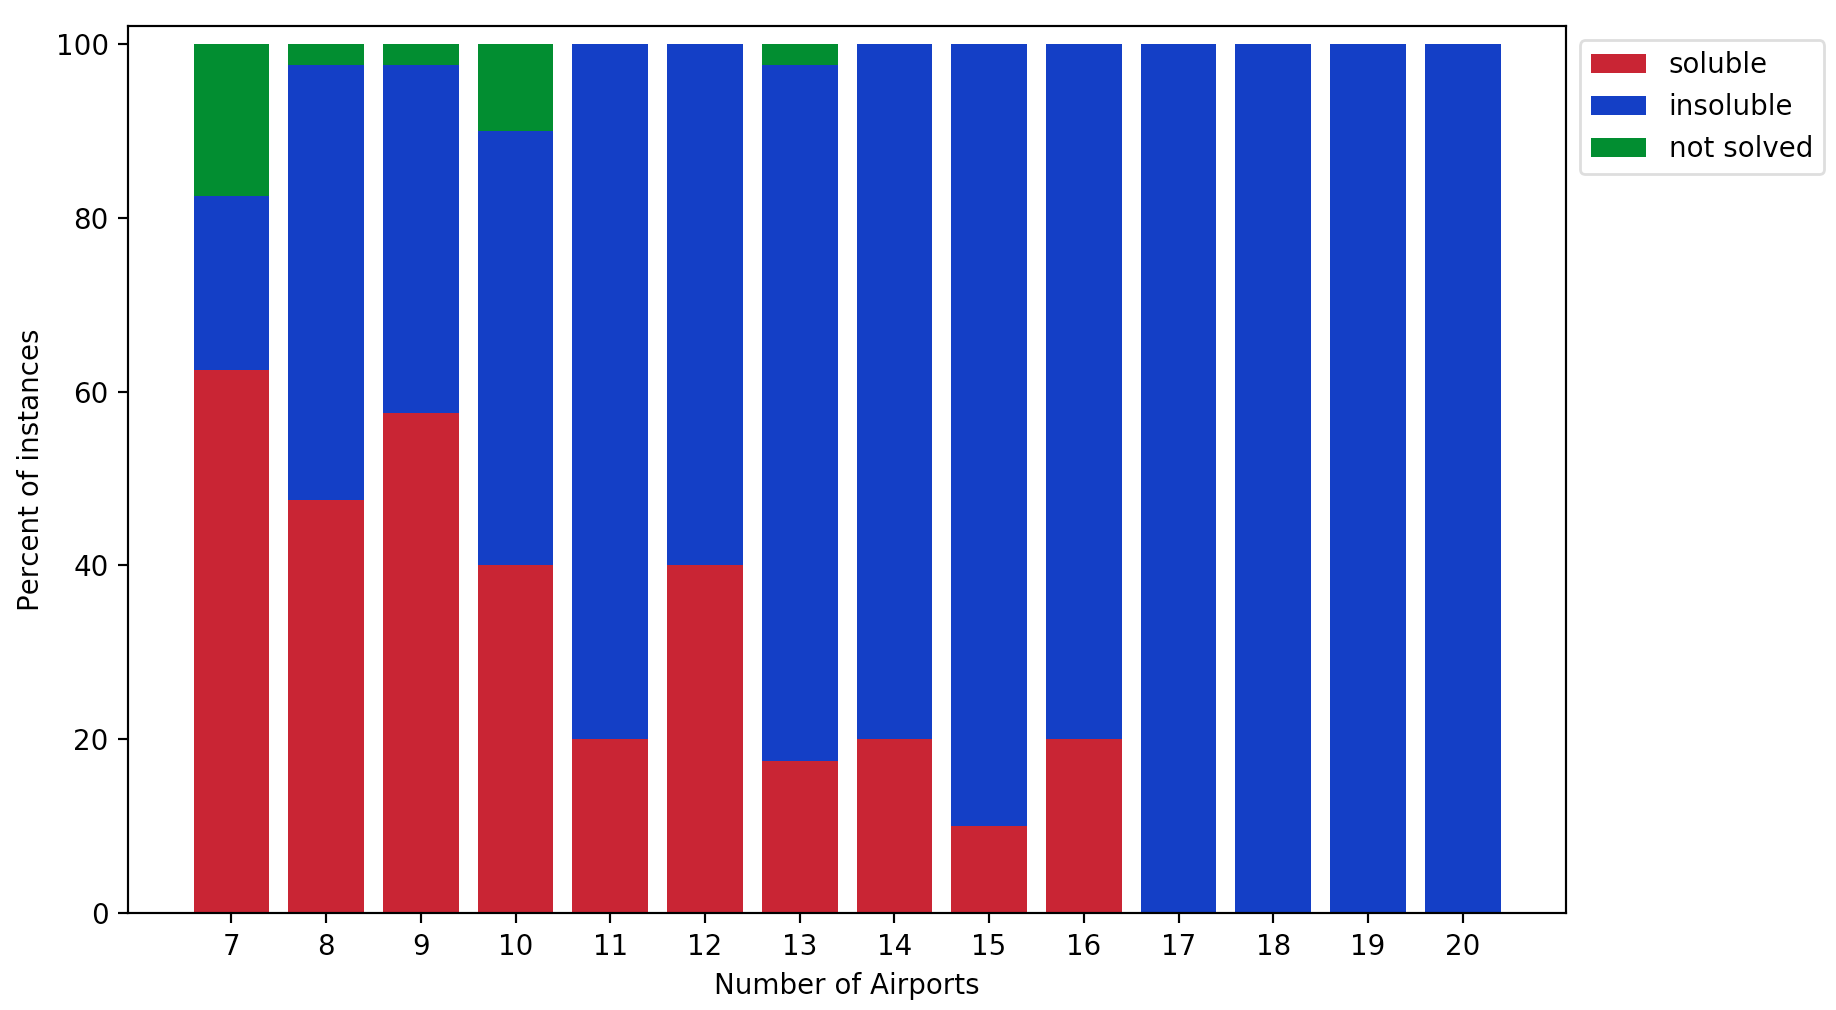
\includegraphics[width=\textwidth, height=4cm]{images/experiments/varyn/varyNsat.png}
        \caption{solubility of trials}
        \label{fig:varynsat}
    \end{subfigure}
    \caption{Experiment 2}
    \label{experiment2}
\end{figure*}
\vspace{-1mm}
%%%%%%%%%%%%%%%%%%%%%%%%
\begin{figure*}[!ht]
    \centering
    \begin{subfigure}[b]{0.30\textwidth}
        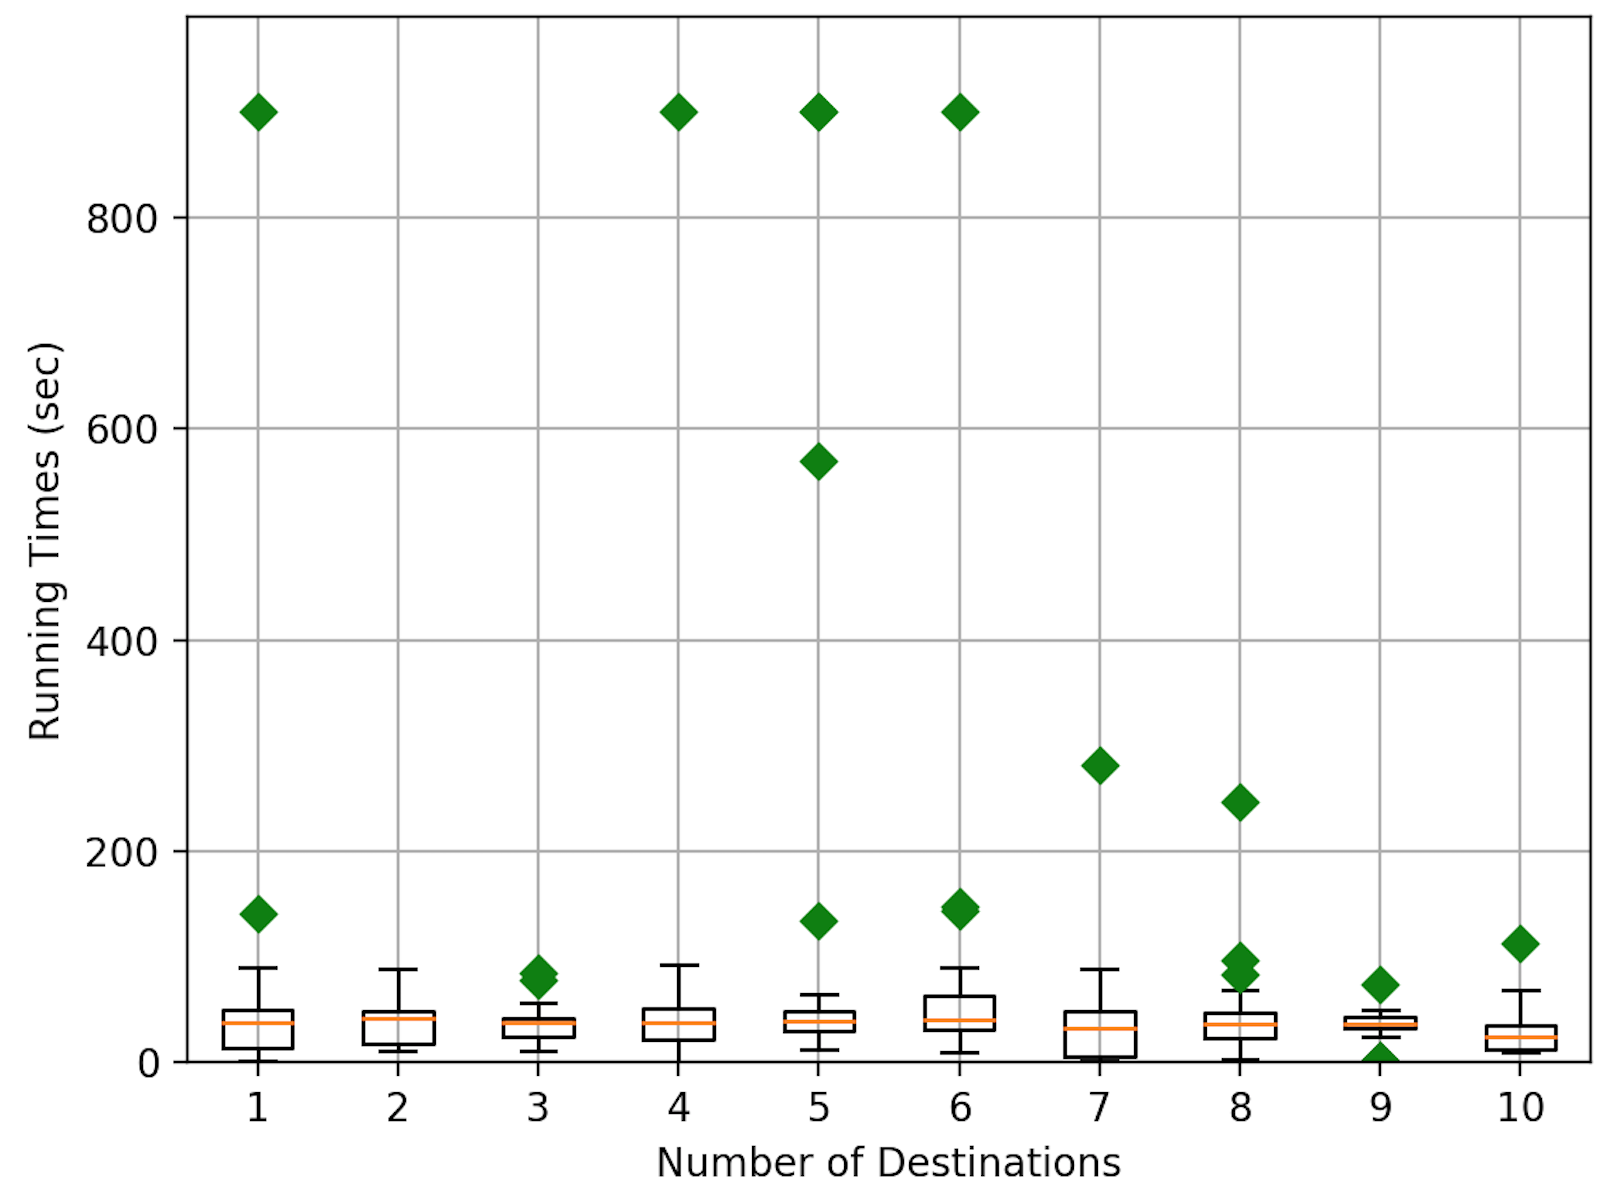
\includegraphics[width=\textwidth, height=4cm]{images/experiments/varyd/varyD.png}
        \caption{all trials}
        \label{fig:exp3all}
    \end{subfigure}
    \begin{subfigure}[b]{0.36\textwidth}
        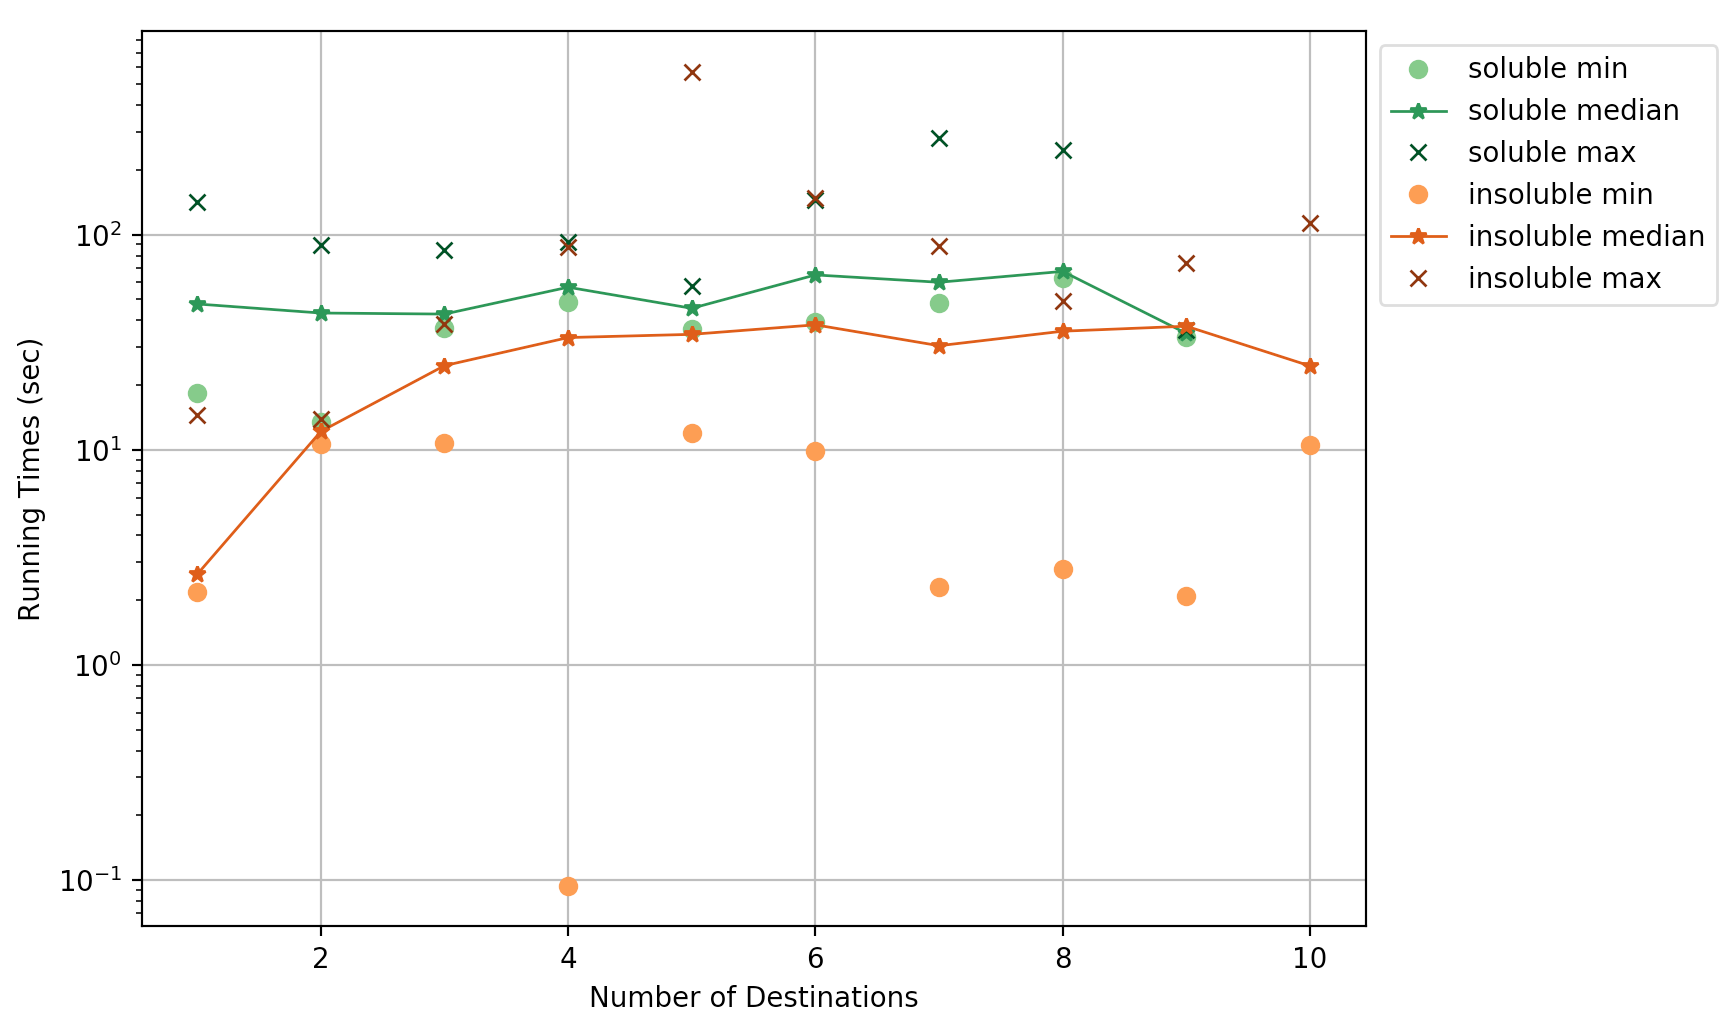
\includegraphics[width=\textwidth, height=4cm]{images/experiments/varyd/satunsat_d.png}
        \caption{soluble vs insoluble trials}
        \label{fig:exp3sat}
    \end{subfigure}
    \begin{subfigure}[b]{0.32\textwidth}
        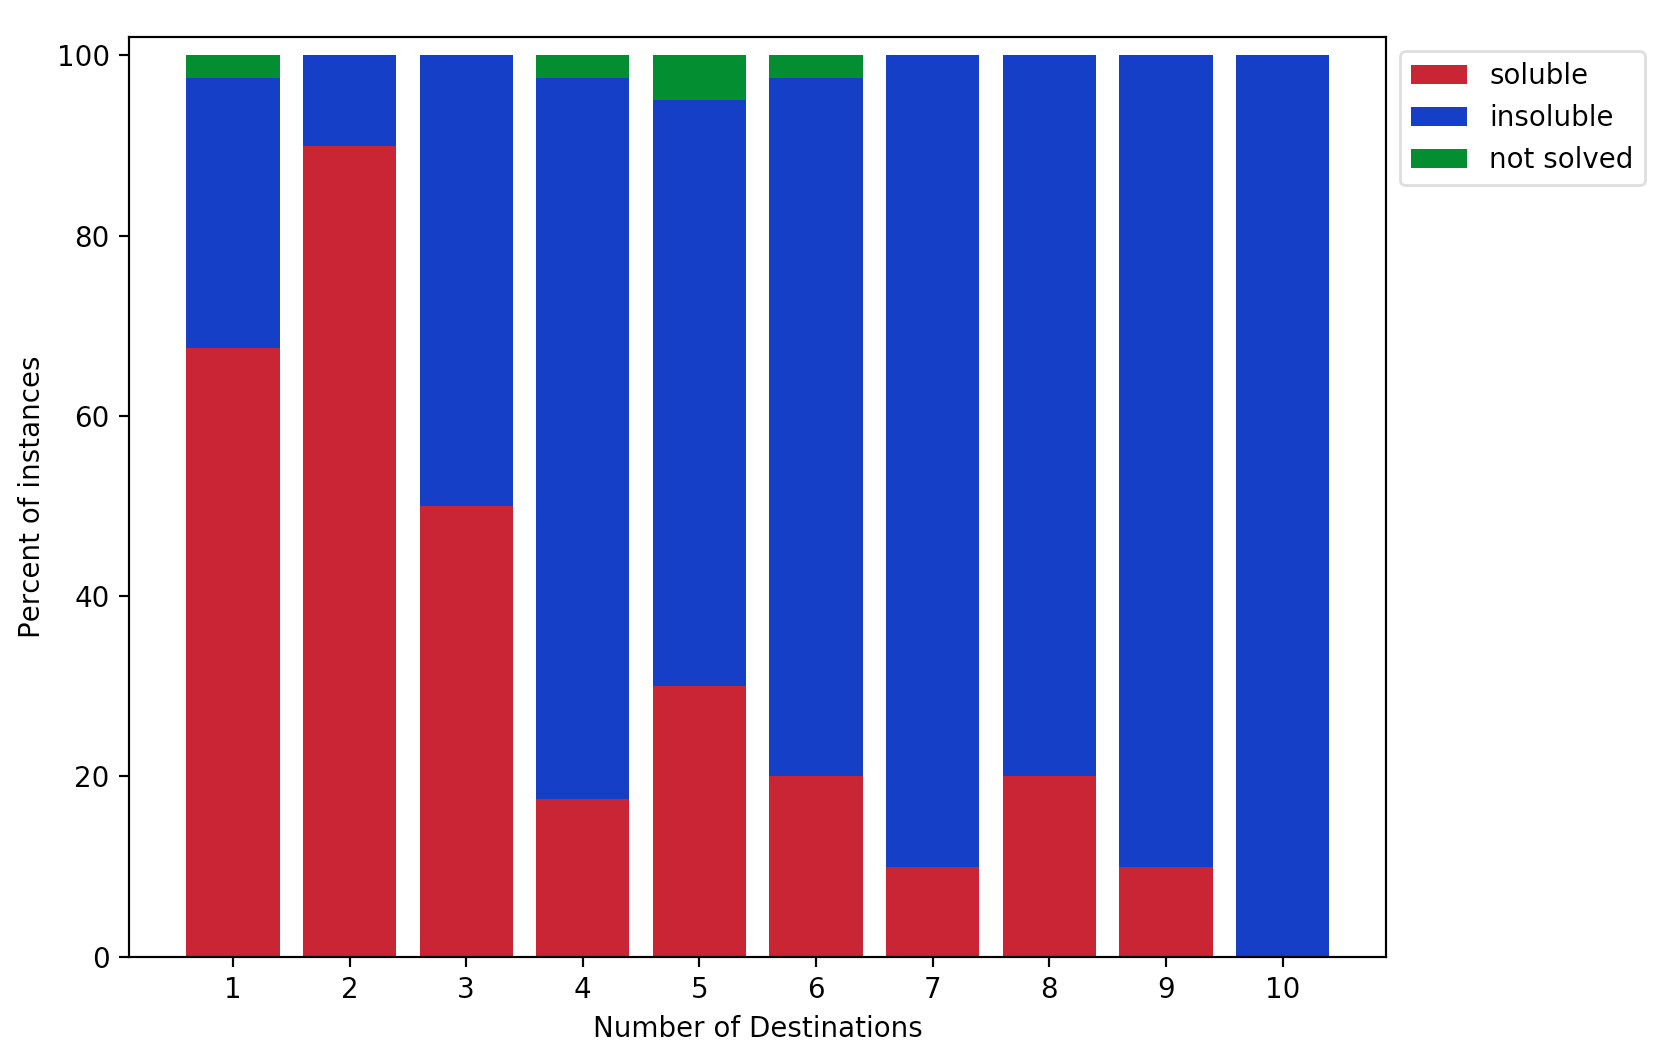
\includegraphics[width=\textwidth, height=4cm]{images/experiments/varyd/varyDsat.png}
        \caption{solubility of trials}
        \label{fig:varydsat}
    \end{subfigure}
    \caption{Experiment 3}
    \label{experiment3}
\end{figure*}
\vspace{-1mm}
%%%%%%%%%%%%%%%%%%%%%%%%
\begin{figure*}[!ht]
    \centering
    \begin{subfigure}[b]{0.30\textwidth}
        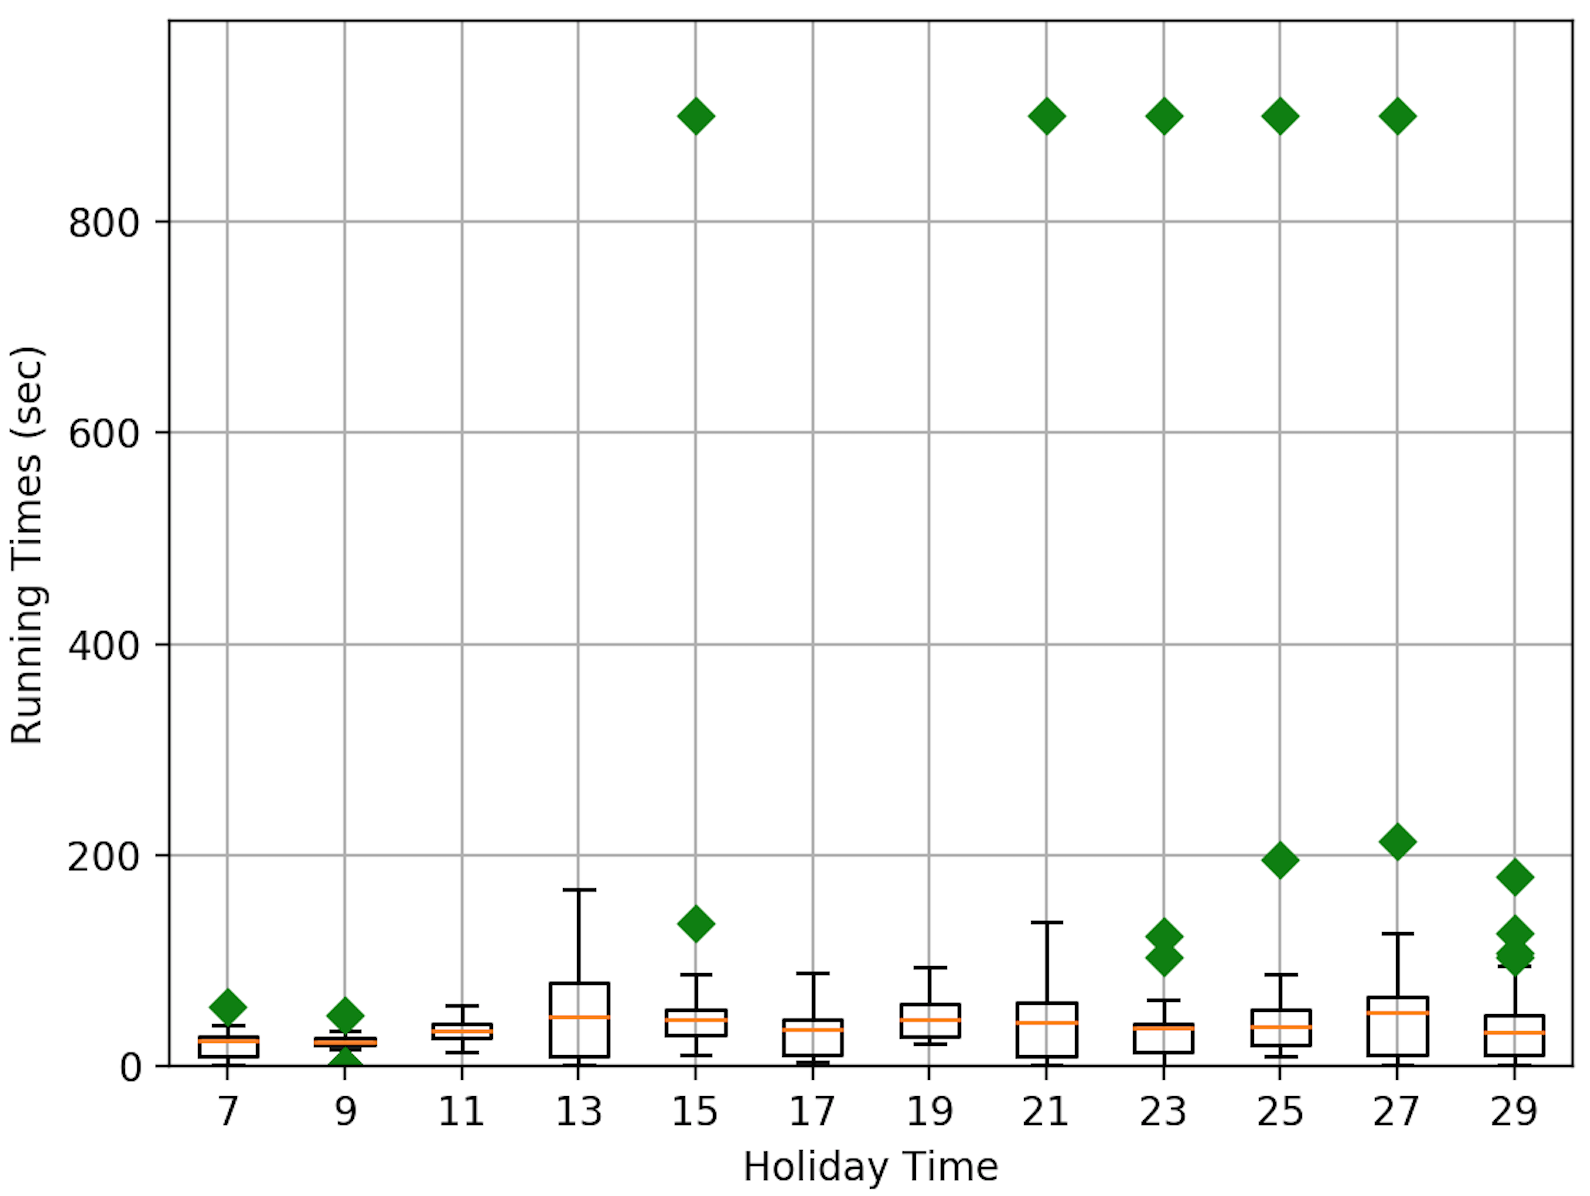
\includegraphics[width=\textwidth, height=4cm]{images/experiments/varyt/varyT.png}
        \caption{all trials}
        \label{fig:exp4all}
    \end{subfigure}
    \begin{subfigure}[b]{0.36\textwidth}
        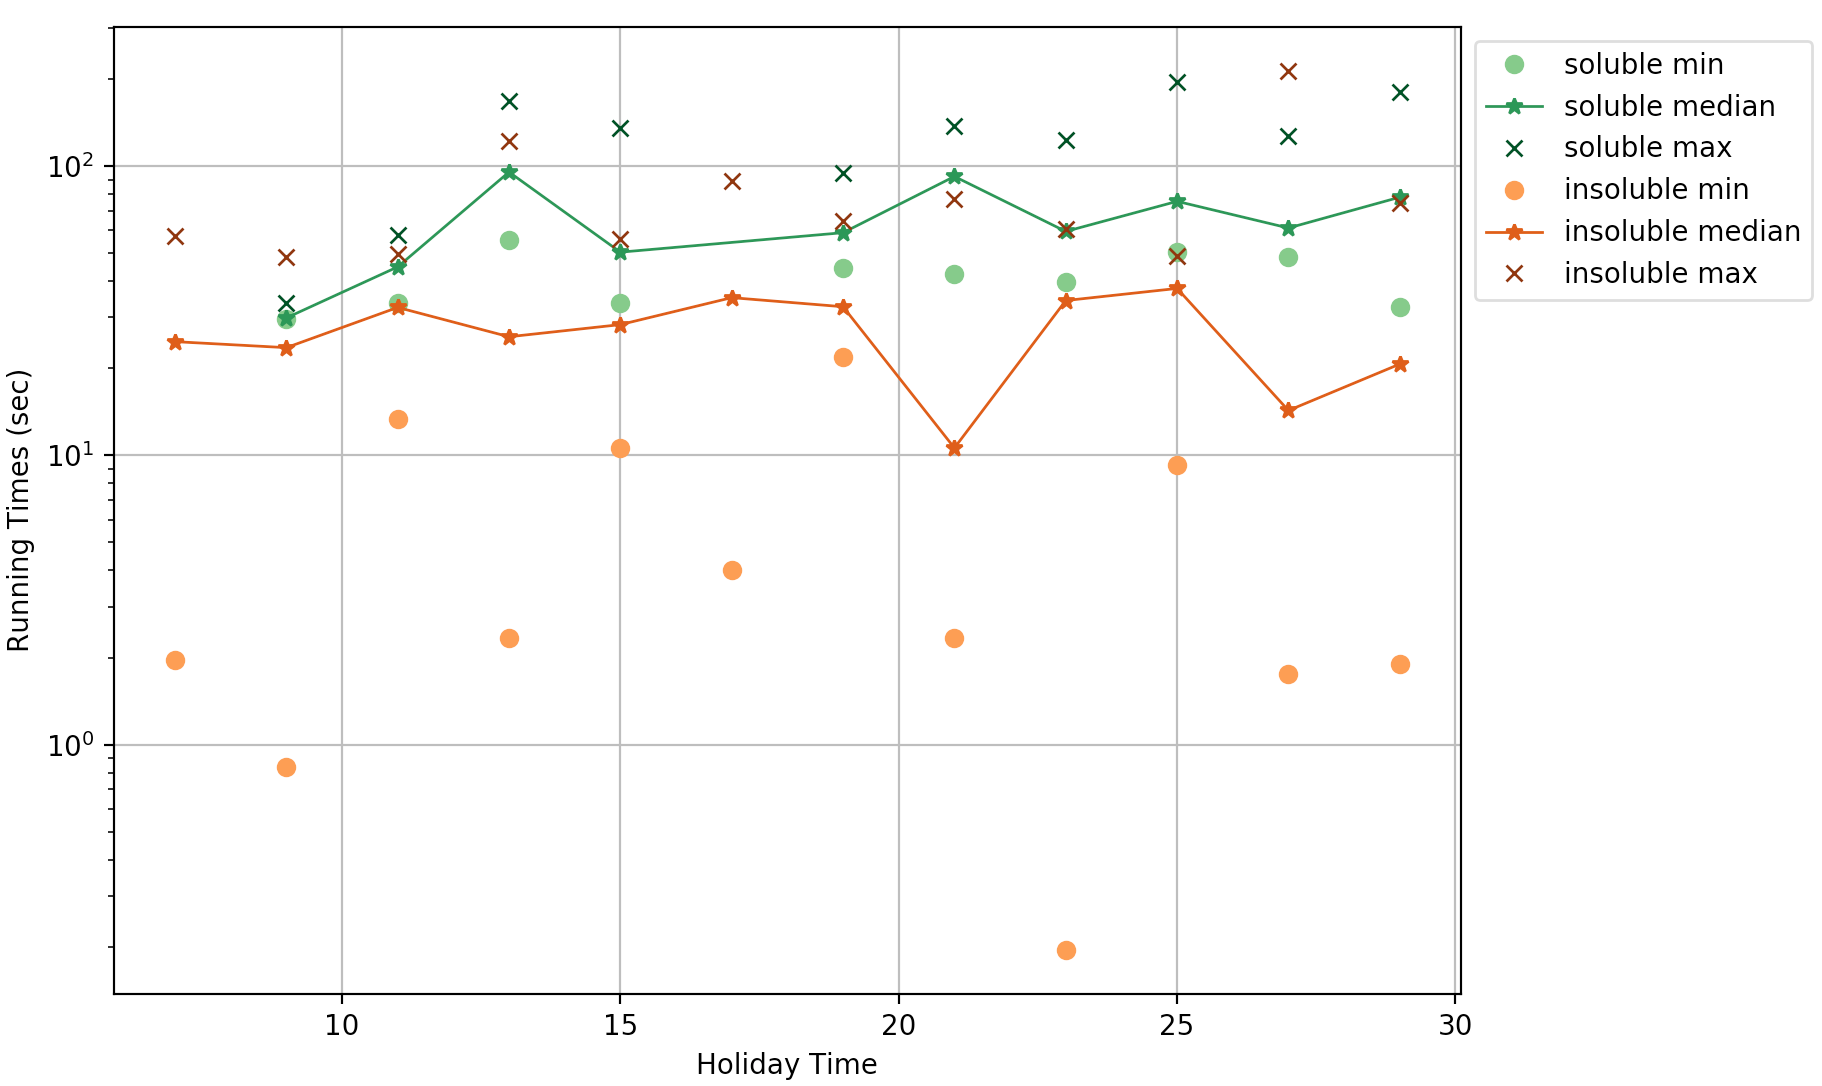
\includegraphics[width=\textwidth, height=4cm]{images/experiments/varyt/satunsat_t.png}
        \caption{soluble vs insoluble trials}
        \label{fig:exp4sat}
    \end{subfigure}
    \begin{subfigure}[b]{0.32\textwidth}
        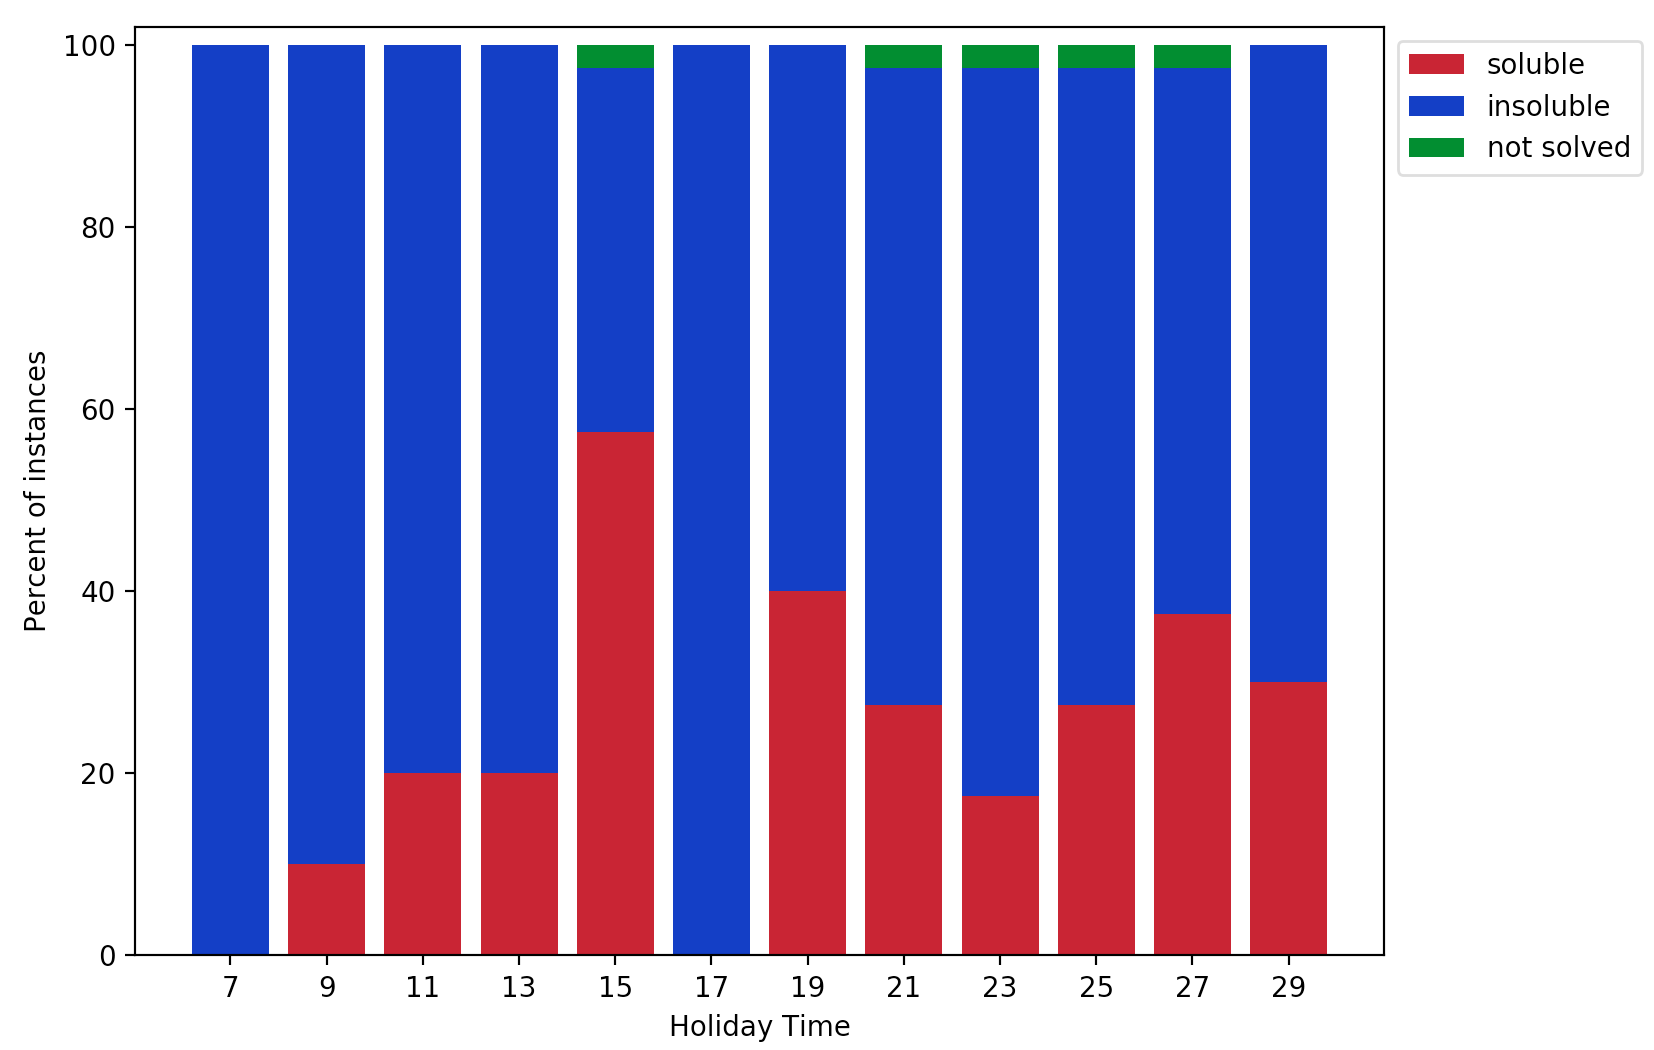
\includegraphics[width=\textwidth, height=4cm]{images/experiments/varyt/varyTsat.png}
        \caption{solubility of trials}
        \label{fig:varytsat}
    \end{subfigure}
    \caption{Experiment 4}
    \label{experiment4}
\end{figure*}
\vspace{-1mm}
%%%%%%%%%%%%%%%%%%%%%%%%

\subsection{Size of real-world TP instances}
\label{tpinstancesize}

Knowing more about the size of the TP instances encountered in reality can give ideas for improvement of the models. This section quantifies \textit{realistic size} in terms of $m$, $n$, $d$ and $T$ using some assumptions and the Skyscanner redirects data.

Let us assume that travellers in Europe typically visit at most 8 destinations, that their holiday lasts for no more than 30 days and that they don't put an upper limit of the number of connecting airports available for usage. The Skyscanner data was used to predict the approximate number of flights $m$ for the assumed values of $n$, $d$ and $T$ as follows. For each value of $d$ $(1 \leq d \leq 8)$, where $n=100$ $T = (d+1) \times 3$ (settings 1-4 in Table \ref{table:testSize}), 50 TP instances were generated and their average, minimum and maximum $m$ was calculated.

Table \ref{table:realisticsize} shows the obtained results: for each value of $d$, $m \sim d^2 \times 100$ on average, where small TP instances tend to have $m \leq 1000$ and large TP instances have $m \sim 7166$. This suggests that the choices of $m$ in Table \ref{table:testSize} were too small. However, the results in Section \ref{experiments:cpvsip} and Section \ref{experiments:ipmodel} show that both models would struggle to solve instances with higher $m$ in terms of $d$.

\vspace{-2mm}
\textcolor{blue}{
\begin{table}[!ht]
\begin{center}
\renewcommand{\arraystretch}{1.2}
\begin{tabular}{|c|c|c|c|c|}
\hline
$d$ & $T$ & Average $m$ & Minimum $m$ & Maximum $m$ \\
\hline
1 & 6  &120.71  	&4       &508 \\
2 & 9  &431.04  	&10      &1,459 \\
3 & 12 &860.2   	&88      &2,879 \\
4 & 15 &1,606.18	&402     &5,213 \\
5 & 18 &2,107.72	&183     &4,784 \\
6 & 21 &3,106.16	&537     &7,010 \\
7 & 24 &4,819.54	&875     &10,786 \\
8 & 27 &7,166.08	&1,506   &13,206 \\
\hline
\end{tabular}
\end{center}
\caption{The minimum, average and maximum number of flights $m$ depending on $d$ and $T$, where $T=(d+1) \times 3$.}
\label{table:realisticsize}
\end{table}}
\vspace{-4mm}

\subsection{Summary of Findings}
\label{experiments:summary}
\vspace{-1mm}
The results from the comparison of the two models show that the
IP model outperforms the CP model and its superiority becomes more evident with the increase of the instance size. Furthermore, the solutions returned by the IP multiobjective optimisation tend to be close to the optimal values, whereas the CP model also returns solutions that have one or more objective values far from the optimum.

It was noted that for $d \geq 7$ most instances were insoluble. This suggests that further empirical evaluation with datasets that consist of higher proportion of soluble instances is needed to determine whether this behaviour is replicated.

The results from the evaluation of the IP model show that $m$ has significant impact on the instance running time, where for TP instances with $m \geq 340$ the IP solver reached the time limit for most trials. This is not surprising. When $m$ is increased, the search space grows in two dimensions for both models: for CP, the size of variables' domains and the number of variables in $\mathcal{S}$ both increase and for IP, this involves creating an additional row and column in the two-dimensional matrix comprising $x_{i,j}$ variables. Therefore, if the same experiments were conducted on the CP model, we would expect to observe similar behaviour.

For each of the evaluated datasets, the IP model is quicker at proving instances as insoluble than solving instances to optimality. This suggests that the solver spends substantial time searching for an optimum, once solubility is proved.

No strong correlation between the running time of the IP solver and the choice of values for $T$ was observed. The running time tends to decrease with the increase of $d$ or $n$, because the number of soluble (that is, ``harder'') instances in the dataset decreases with the increase of $d$ or $n$.

% aims to answer the following question: can the models solve TP instances of \textit{realistic} size \textit{quickly enough}?
We also estimated the size of real-world TP instances using the Skyscanner data. The results show the following relation between $m$ and $d$: $m \sim d^2 \times 100$, which means that at their current state, both models are too inefficient to solve real-world TP instances as part of a real-time application. Improving their efficiency requires reducing the influence of $m$ on their time complexity.

\section{Conclusion and Future Work}
\label{conclusionandfuturework}

This work investigated the Traveller's Problem (TP): a combinatorial optimisation problem that finds direct applications in the travel industry.
We constructed two algorithms for solving TP and some of its extensions and variations. The algorithms use Integer Programming (IP) and Constraint Programming (CP) and both can return optimal solutions subject to four objectives: cost, number of connecting airports, trip duration, number of flights, as well as any combination of them. In addition, the CP model implements two hard constraints that a TP solution may be required to satisfy.

The author of this project was given access to flight booking data for the period of half a year by Skyscanner; a travel metasearch engine widely used for booking itineraries online. The utilisation of this data involved building a framework for processing the data and creating TP instances from it.

The evaluation was performed on each model with TP instances generated from Skyscanner data. The results show that the IP is much quicker at solving problems than the CP model, where the difference between their running times increases with the increase of the instance size. The time complexity of both models is highly influenced on the number of flights in the instance and this makes them too inefficient to solve real-world TP instances, where it was observed that $m \sim d^2 \times 100$. 

Future work should aim to build an algorithm for solving real-world TP instances. Achieving this milestone is worthwhile, because it will have a significant impact on the travel metasearch industry and will improve travelling and trip planning experience of travellers around the world.
The rest of this section gives suggestions for improving and evaluating the models.

An alternative way to model TP is to have all destinations as decision variables instead of flights. For example, the CP model can have an array $\mathcal{D}$ of $d$ variables that denotes the order in which the destinations are visited for the first time, where the domain of each variable is $(1,...,d)$. For example, having $\mathcal{D}[i] = j$ would mean that destination with id $j$ is the $i^{th}$ visited destination, given that each destination has a unique integer from $1$ to $d$ assigned as an id.

Both models do not implement any heuristics and both solvers execute default search algorithms (Section \ref{sec:solvers}). Existing work has shown that the choice of heuristics can have significant impact on the search effort \cite{Haralick80:a, Gent96,Christopher03}. Future work should investigate existing heuristics and search strategies and look into developing specialised versions for TP.

In order to reduce the size of the search space, each TP instance can be preprocessed before its model is created. Preprocessing can consist of concatenation of pairs of flights as follows: let $f_j$ and $f_k$ be two flights having $A^a_j = A^d_k = A_i$ for $A_i \notin D$ and $t_j + \Delta_j + C_{A^a_j} \leq t_k$. Then a new flight $f_{j,k}$ called a \textit{meta-flight} can be constructed with $A^d_{j,k} = A^d_j$, $A^a_{j,k} = A^a_{k}$, $t_{j,k} = t_{j}$, $\Delta_{j,k} = t_k - t_j + \Delta_k$ and $c_{j,k} = c_j + c_k$. This process is repeated for the concatenated flights until a new set $F^\prime$ of flights only to and from destinations is obtained. Creating meta-flights removes the need to model connecting airports and potentially reduces the number of flights in the instance. However, it requires storing extra data, such as the set of flights each meta-flight is composed of (if solution with minimum number of flights is required). Future work should further investigate this idea and its trade-offs.

%% todo: future work should evaluate soft and hard constraints

% I would have liked to see a study where feasible solutions were generated and then a problem built around them, so that we have a class of problems that we know are soluble/feasible
During evaluation, we repeatedly encountered the issue of having too few soluble TP instances for high values of $d$. In future work, modifying the TP instance generator to build trips from the Skyscanner data and then build TP instances around these pre-generated trips could solve this issue.

% It would be nice to have soluble instances (as above) an amount of time and report the quality of solution found. We might then vary cpu time and ask “Given t seconds, how good a solution can we find?'
In real-world applications, incumbent solutions that are sufficiently close to the optimum are often accepted. Future work can investigate the trade-off between the quality of the incumbent solution and the time taken to compute it. This can be done by repeatedly solving a set of soluble instances, each time varying the imposed time limit $t$ and calculating the scores of the returned solutions using Equation \ref{eq:score}.

\clearpage

\bibliographystyle{plainnat}
\bibliography{example}

% \clearpage

\appendix

\section{Complexity of TP}
\label{appendix:tpcomplexity}
\begin{theorem}
TPD is NP-complete.
\end{theorem}

\begin{proof}
This proof first shows the membership of TPD in the NP class of problems. Second, we prove the NP-hardness of TP by constructing a polynomial-time reduction from a known NP-complete problem $\Pi$ to TPD, where $\Pi$ is chosen to be TSP, defined in Section \ref{npcompleteproblems}. Its NP-hardness follows by a reduction from the Hamiltonian Cycle problem. The proof is presented by
\cite{thebible}.

Given an instance of TPD and $s$, which is a sequence of flights from $F$, we can write an algorithm that checks in polynomial time whether $s$ is a solution. To accept or reject validity, the algorithm only needs to traverse $s$ and check that it satisfies all required properties. Therefore, TP is in NP.

Let $\pi$ be an instance of TSP. Let $\pi^{\prime}$ be an instance of TPD with the following properties:
\begin{itemize}
\item The set of airports in $\pi^{\prime}$ is identical to the set of cities in $\pi$ and it is similarly denoted as $A$ (a city in $\pi$ is called an airport in $\pi^{\prime}$). Airport $A_{1}$ is the home airport.
\item Each airport in $A$ is also a destination.
\item The connection time $C_{A_{i}}$ for each airport $A_{i}$ is equal to 0.
\item $T$ is equal to $n$.
\item Let $C$ be the Cartesian product of the airports in $A$ with itself, that is $C = A \times A$ = \{($A_{i}, A_{j}$) : $A_{i}$ $\in$ $A$, $A_{j}$ $\in$ $A$, $i \neq j$\}. Then $F$ is a set of flights, such that for every ($A_{i}, A_{j}$) $\in$ $C$, there exists a flight $f_{k}$ in $F$, such that $A^{d}_{k} = A_{i}$ and $A^{a}_{k} = A_{j}$ for every date $0 \leq t < T$.
\item For every $f_{k}$ $\in$ $F$, $c_{k}$ is equal to $d(A^{d}_{k}, A^{a}_{k})$ in $\pi$. Therefore, the flight costs also satisfy the triangle inequality.
\item For every $f_{k}$ $\in$ $F$, $\Delta_{k}$ = 1.
\item $B$ is the upper bound on the allowed total cost.
\end{itemize}

%% TSP solution => also TP solution

Suppose that $\gamma$ = $ \langle A_{i_{1}}, A_{i_{2}},...,A_{i_{n}} \rangle $ is a solution to $\pi$, where $\langle i_{1},...,i_{n} \rangle$ is a permutation of $\langle 1,...,n \rangle $ and the total travel distance $L_{\gamma} \leq B$. Without loss of generality, assume that $i_{1} = 1$. In $\pi^{\prime}$, $\gamma$ is equivalent to the order of visited airports by some sequence of flights $s$ = $ \langle f_{j_{1}}, f_{j_{2}},...f_{j_{n}} \rangle $, such that for each $p$  $(1 \leq p \leq n)$ there exists $q$ $(1 \leq q \leq n)$ such that $A^{d}_{j_{q}} = A_{i_{p}}$ and $A^{a}_{j_{q}} = A_{i_{p+1}}$, where subscripts are taken modulo $n$. Therefore, $s$ satisfies property (1) of a valid solution. For each $q$ $(1 \leq q \leq n)$, $A^{a}_{j_{q}} = A^{d}_{j_{q+1}}$ and $t_{j_{q}} = q - 1$.  We know that such flights exist in $F$ by the construction of the set $F$.

From the construction of $s$, it follows that property (2) also holds. Properties (3) and (4) also hold, since we have chosen flights from $F$ such that for every $f_{j_{q}}$ $\in$ $s$, $t_{j_{q}} = q - 1$ ($(1 \leq q \leq n)$). Property (5) is satisfied, since all airports in $A$ are destinations.

Since the cost of every flight in $F$ is equal to the distance between the two cities in $\pi$ that correspond to its departure and arrival airport, it follows that $c(s) = L_{\gamma} \leq B$.

The sequence $s$ satisfies all requirements for a valid solution to $\pi^{\prime}$. Therefore, a solution of $\pi$ is also a solution to $\pi^{\prime}$.

Conversely, suppose that $s = \langle f_{j_{1}},...,f_{j_{k}} \rangle $ is a solution to $\pi^{\prime}$, where the flights in $s$ visit destinations in the sequence $\gamma^{\prime}$ = $\langle A_{i_{1}}, A_{i_{2}},...,A_{i_{m}} \rangle$. We will prove that $\gamma^{\prime}$ is a solution of $\pi$.

By construction of $\pi^{\prime}$, all airports in $A$ are also destinations. Therefore, $\gamma^{\prime}$ contains all cities in $A$, that is $m \geq n$. Suppose that $m > n$ and an arbitrary airport $A_{p}$ $(1 \leq p < n)$ is included more than once in $\gamma^{\prime}$. Then $s$ must contain more than one flight with arrival airport equal to $A_{p}$. 
The duration of each flight in $\pi^{\prime}$ is one day. Therefore, for every $q$ $(1 \leq q < n - 1)$, $t_{j_{q+1}} = q$. Since the traveller has only $n$ days of total travel time, and $s$ is restricted to contain exactly $n$ flights, that is $k = n$. The only way to visit $n$ distinct destinations, given $n$ flights is that all flights in $s$ have unique arrival airports. Assuming that $A_{p}$ is visited more than once means that there is more than one flight with arrival airport equal to $A_{p}$, which is a contradiction. Therefore, $m = n$ and each airport in $A$ is visited exactly once.

From the properties of $s$ it follows that $A^{d}_{j_{1}} = A^{a}_{j_{n}} = A_{1}$. Therefore, $\gamma^{\prime}$ is a cycle of size $n$. We know that $c(s) \leq B$. We assigned a cost of each flight $f_{k}$ in $F$ to be equal to $d(A^{d}_{k}, A^{a}_{k})$ in $\pi$. Therefore, the total travel distance $L_{\gamma^{\prime}} = c(s)$ which is less than or equal to $B$.

According to the specifications of $\pi$, $\gamma^{\prime}$ is a solution to $\pi$. Therefore, a solution to $\pi^{\prime}$ is also a solution to $\pi$.

The transformation from a TSP instance to an instance of TPD can be done in polynomial time. For each of the $n$($n$-1)/2 distances d($A_{i}$, $A_{j}$) that must be specified in $\pi$, it is sufficient to check that the same cost is assigned to the flights from $A_{i}$ to $A_{j}$ for all dates.

Therefore, TP is in NP and the decision version of TSP can be reduced to TPD in polynomial time, from which it follows that TPD is NP-complete.
\end{proof}

\section{Additional Evaluation results}
\label{appendix:evaluation}

\begin{figure*}
    \centering
    \begin{subfigure}[b]{0.22\textwidth}
        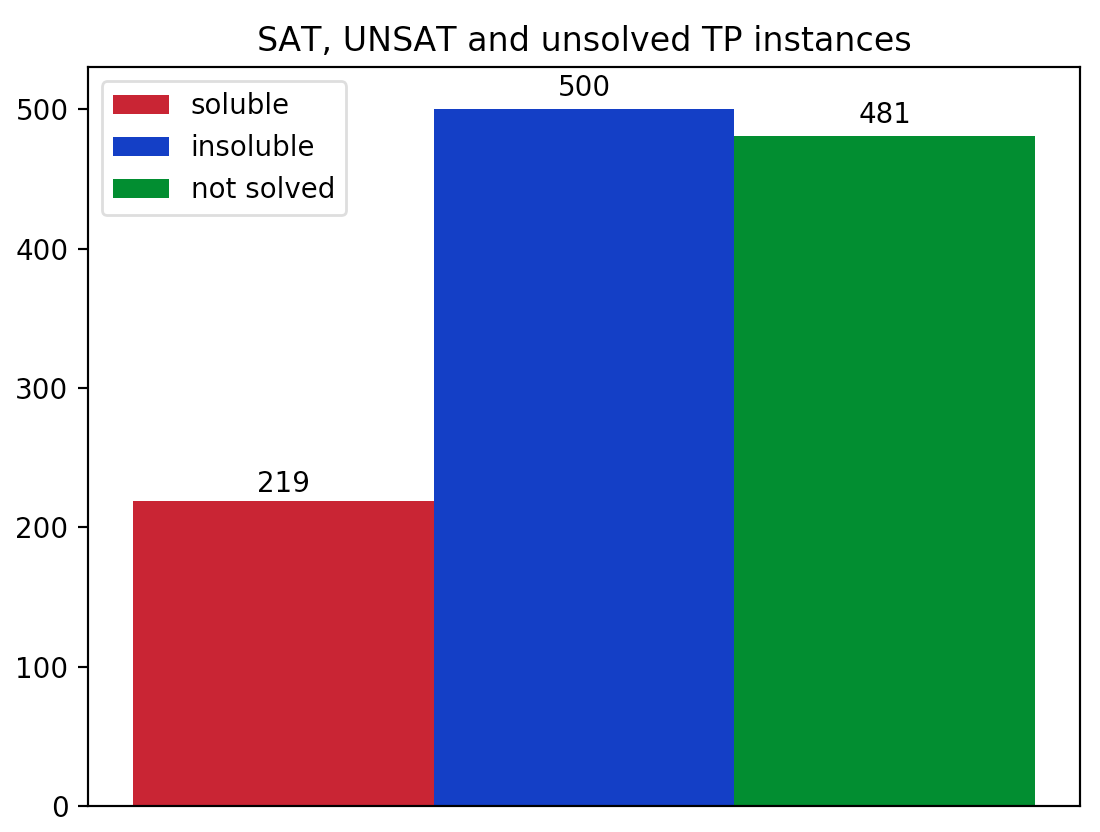
\includegraphics[width=\textwidth, height=4cm]{cpipexperiments/cp_d.png}
        \caption{CP $\mathcal{D}_3$}
        \label{fig:cp_d}
    \end{subfigure}
    \begin{subfigure}[b]{0.22\textwidth}
        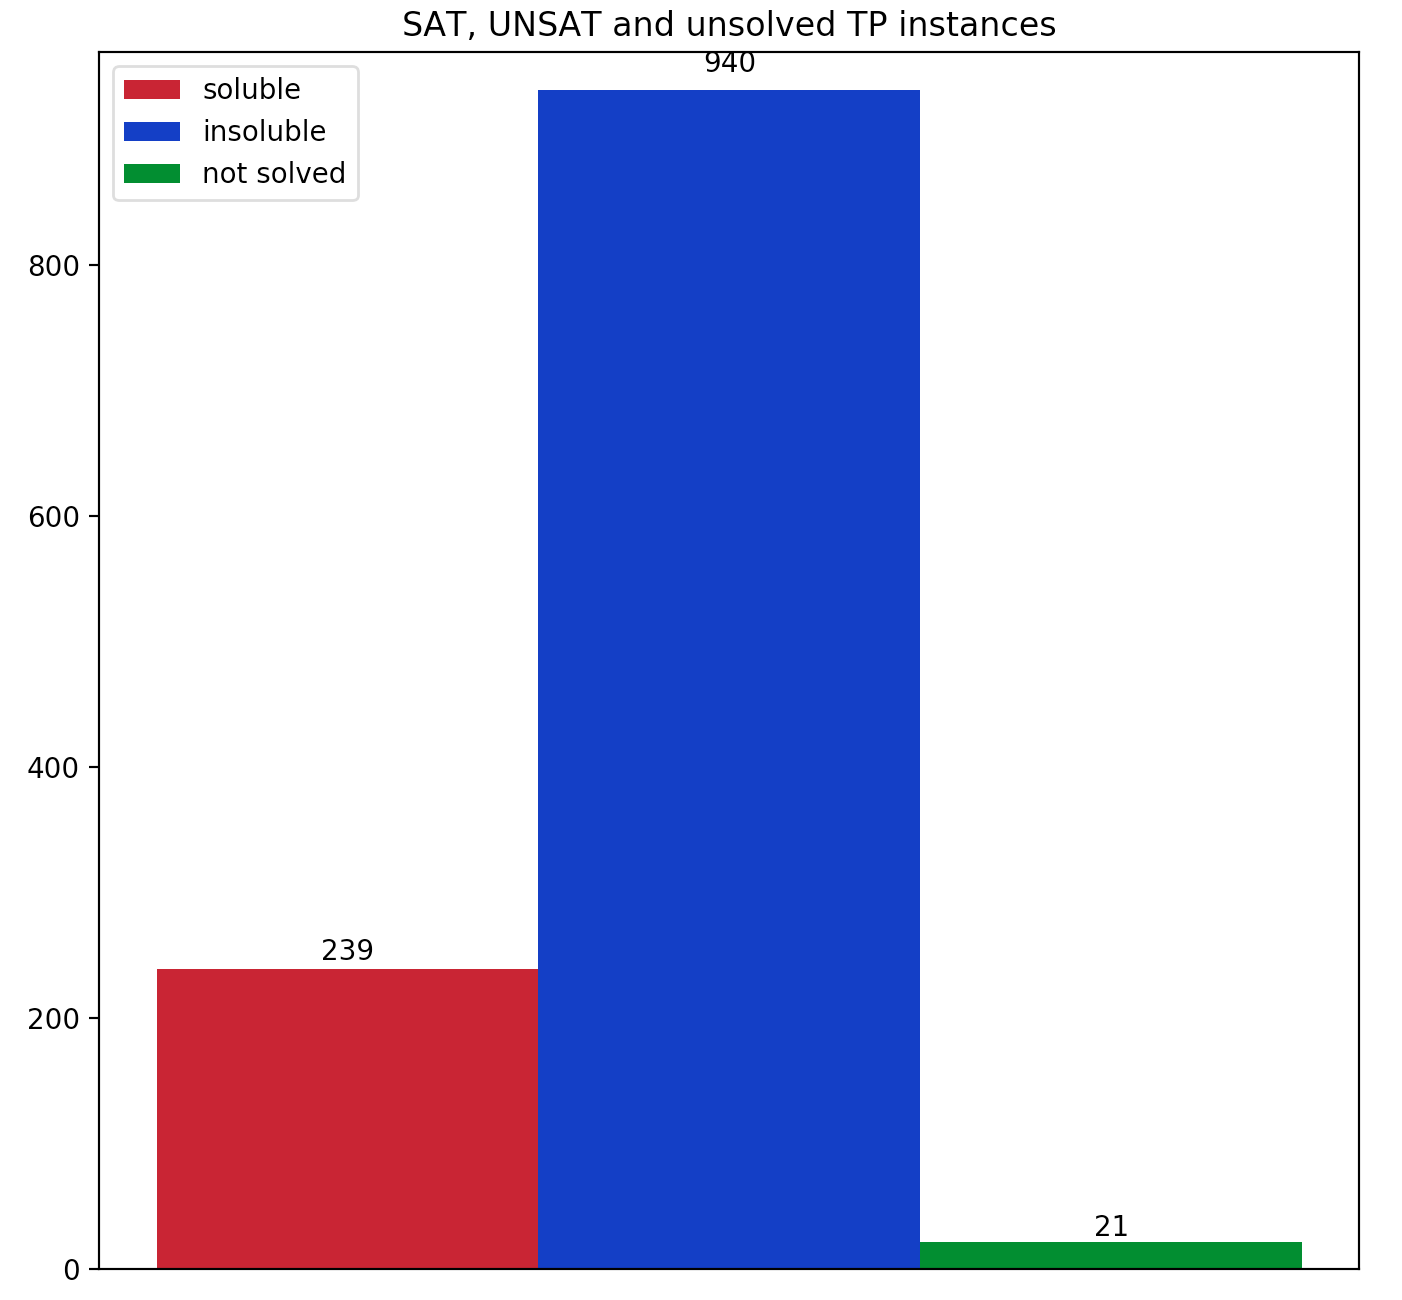
\includegraphics[width=\textwidth, height=4cm]{cpipexperiments/ip_d.png}
        \caption{IP $\mathcal{D}_3$}
        \label{fig:ip_d}
    \end{subfigure}
    \begin{subfigure}[b]{0.22\textwidth}
        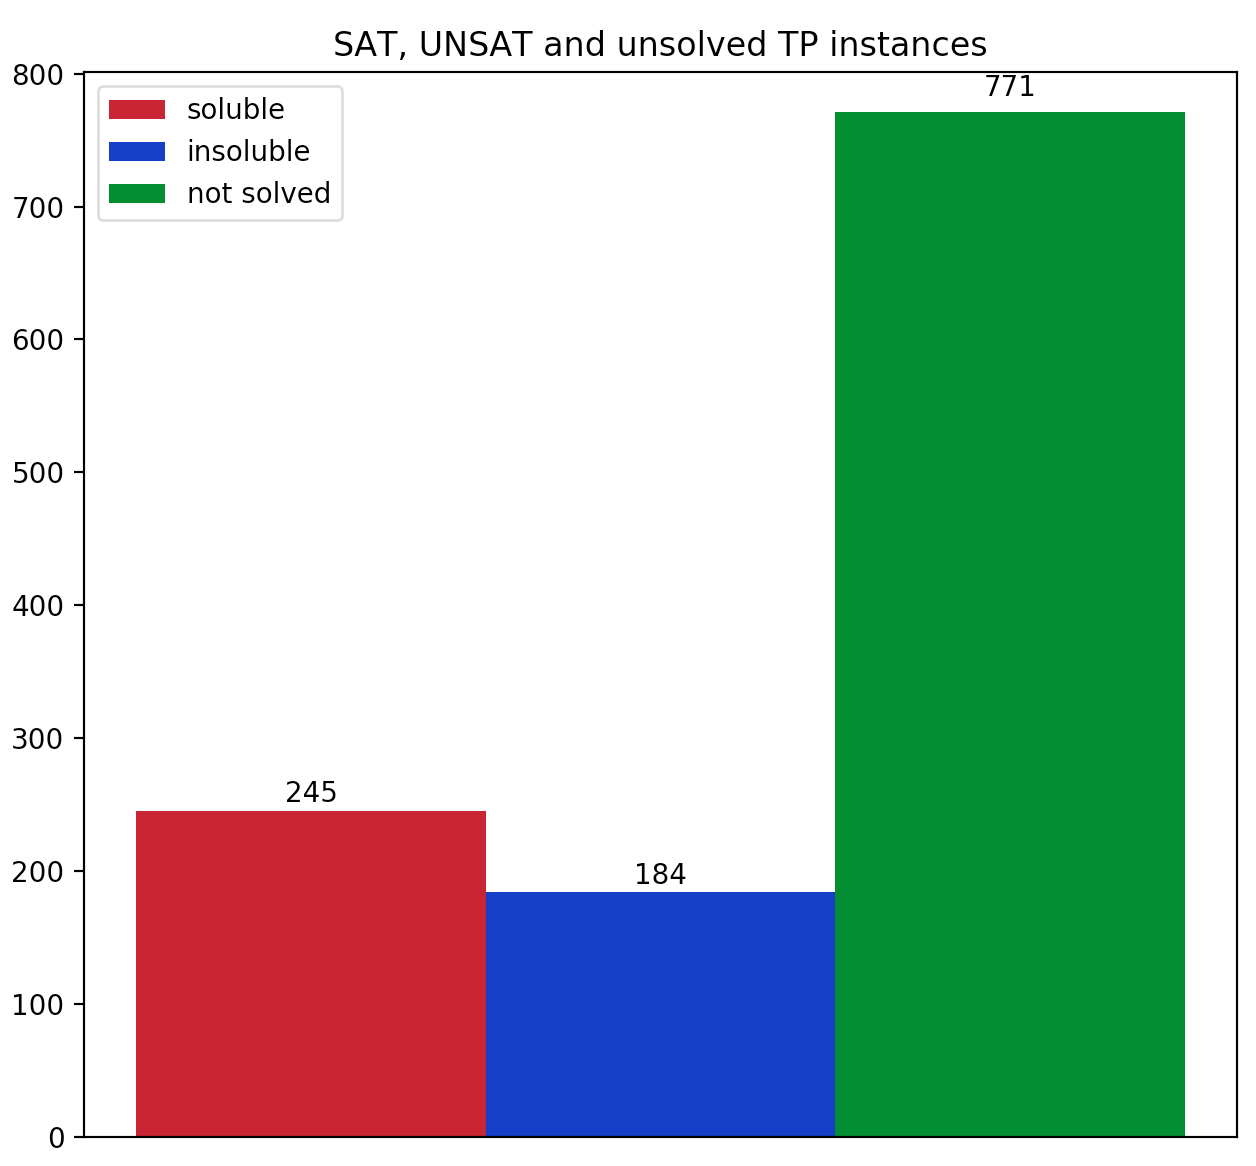
\includegraphics[width=\textwidth, height=4cm]{cpipexperiments/cp_d2.png}
        \caption{CP $\mathcal{D}_4$}
        \label{fig:cp_d2}
    \end{subfigure}
    \begin{subfigure}[b]{0.22\textwidth}
        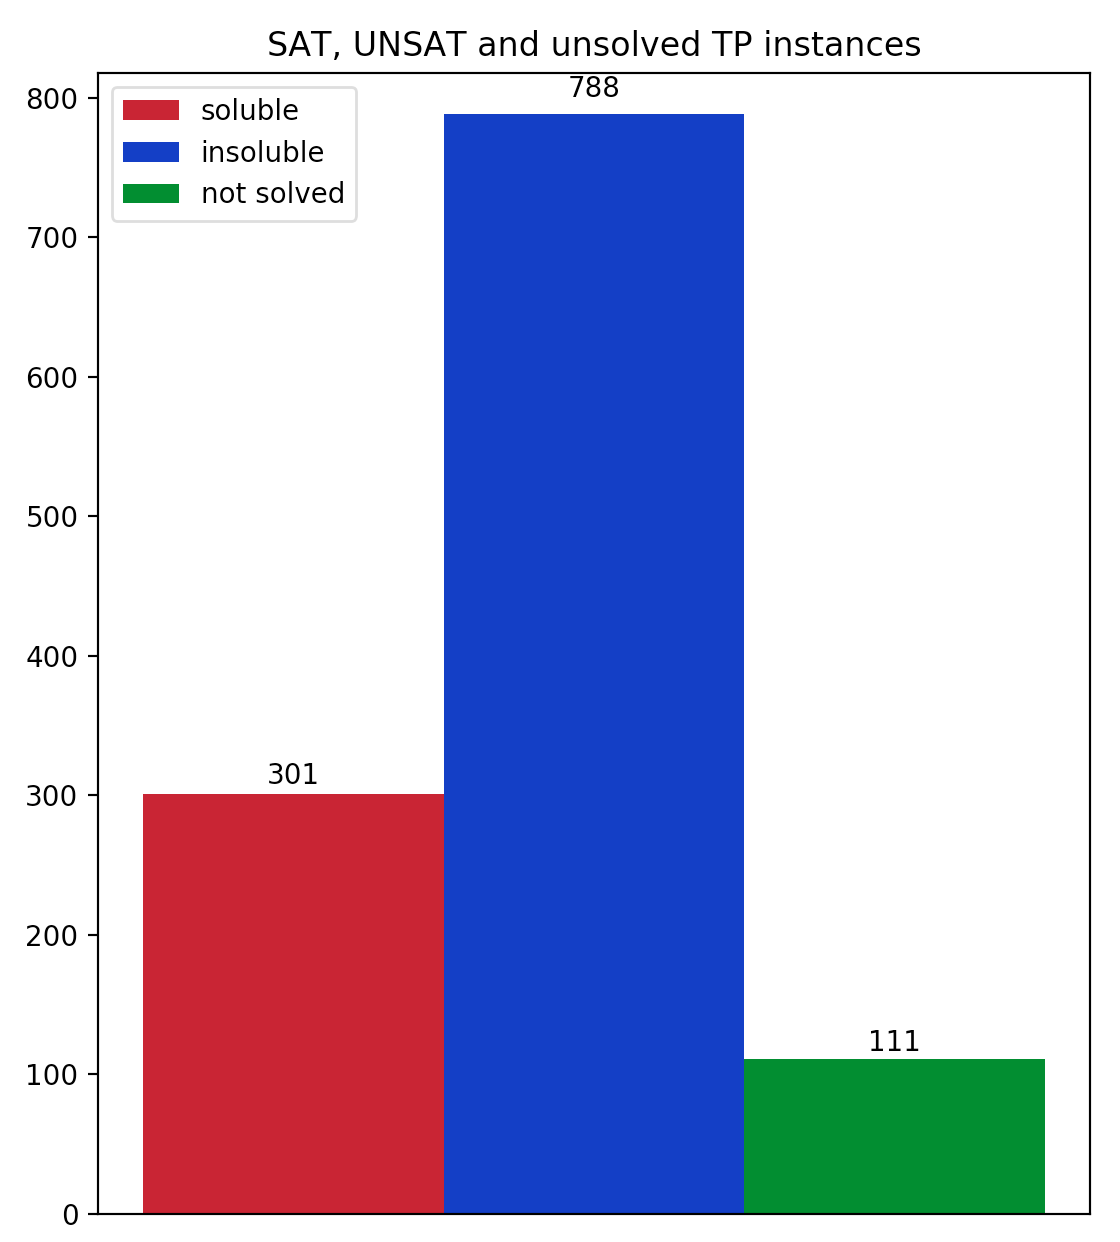
\includegraphics[width=\textwidth, height=4cm]{cpipexperiments/ip_d2.png}
        \caption{IP $\mathcal{D}_4$}
        \label{fig:ip_d2}
    \end{subfigure}
    \caption{The number of soluble, insoluble and not solved trials for each model and dataset.}
    \label{fig:dandd2solvability}
\end{figure*}

\begin{figure*}
    \centering
    \begin{subfigure}[b]{0.48\textwidth}
        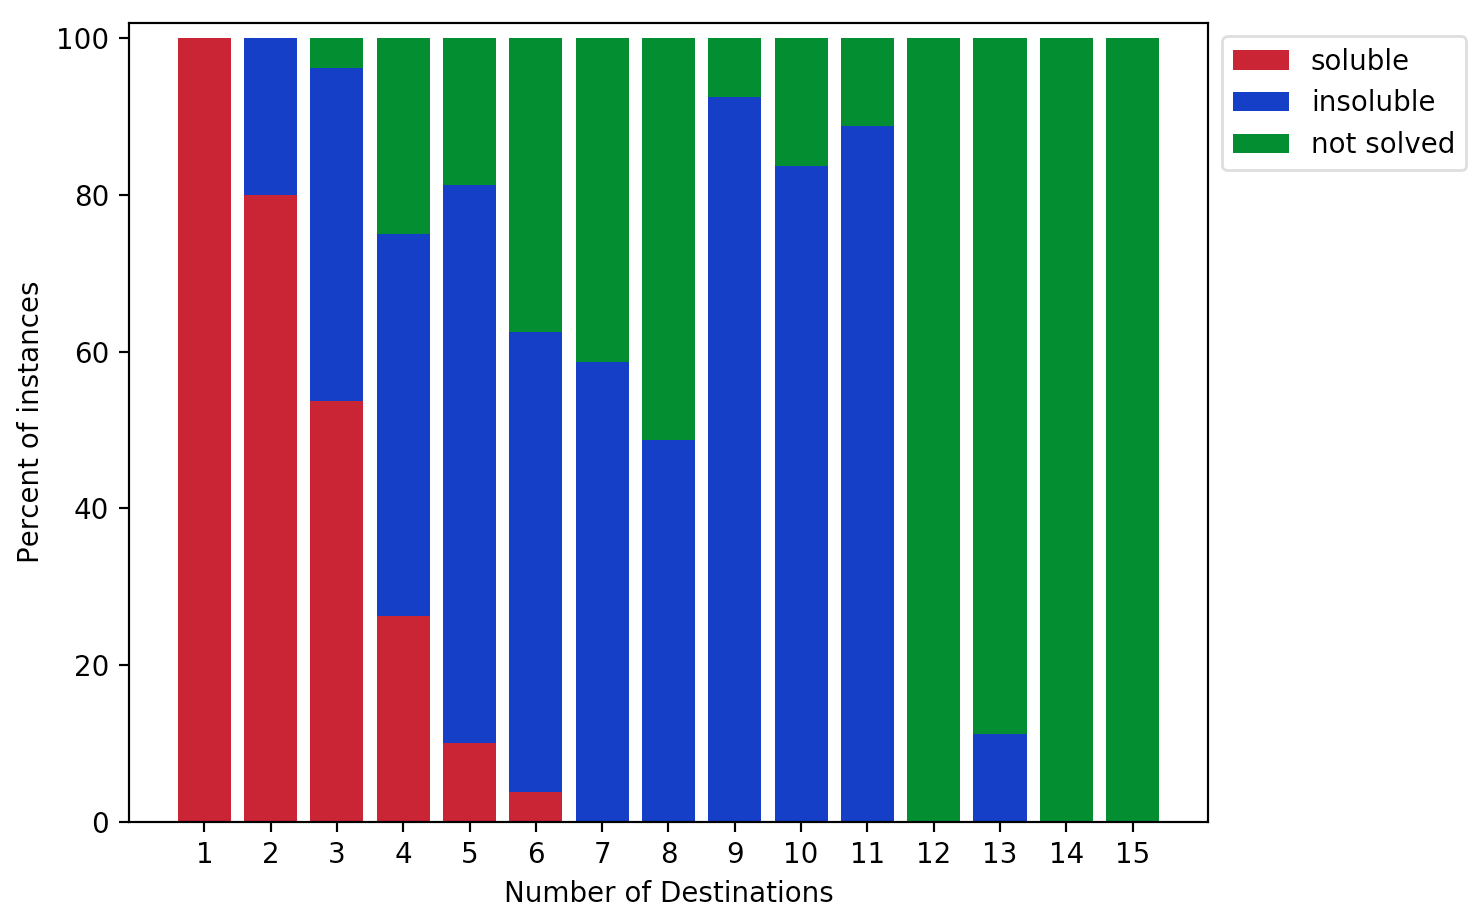
\includegraphics[width=\textwidth, height=5cm]{cpipexperiments/satunsatnotsolved_cp_d.png}
        \caption{CP $\mathcal{D}_3$}
        \label{fig:satunsatnotsolved_cp_d}
    \end{subfigure}
    \begin{subfigure}[b]{0.48\textwidth}
        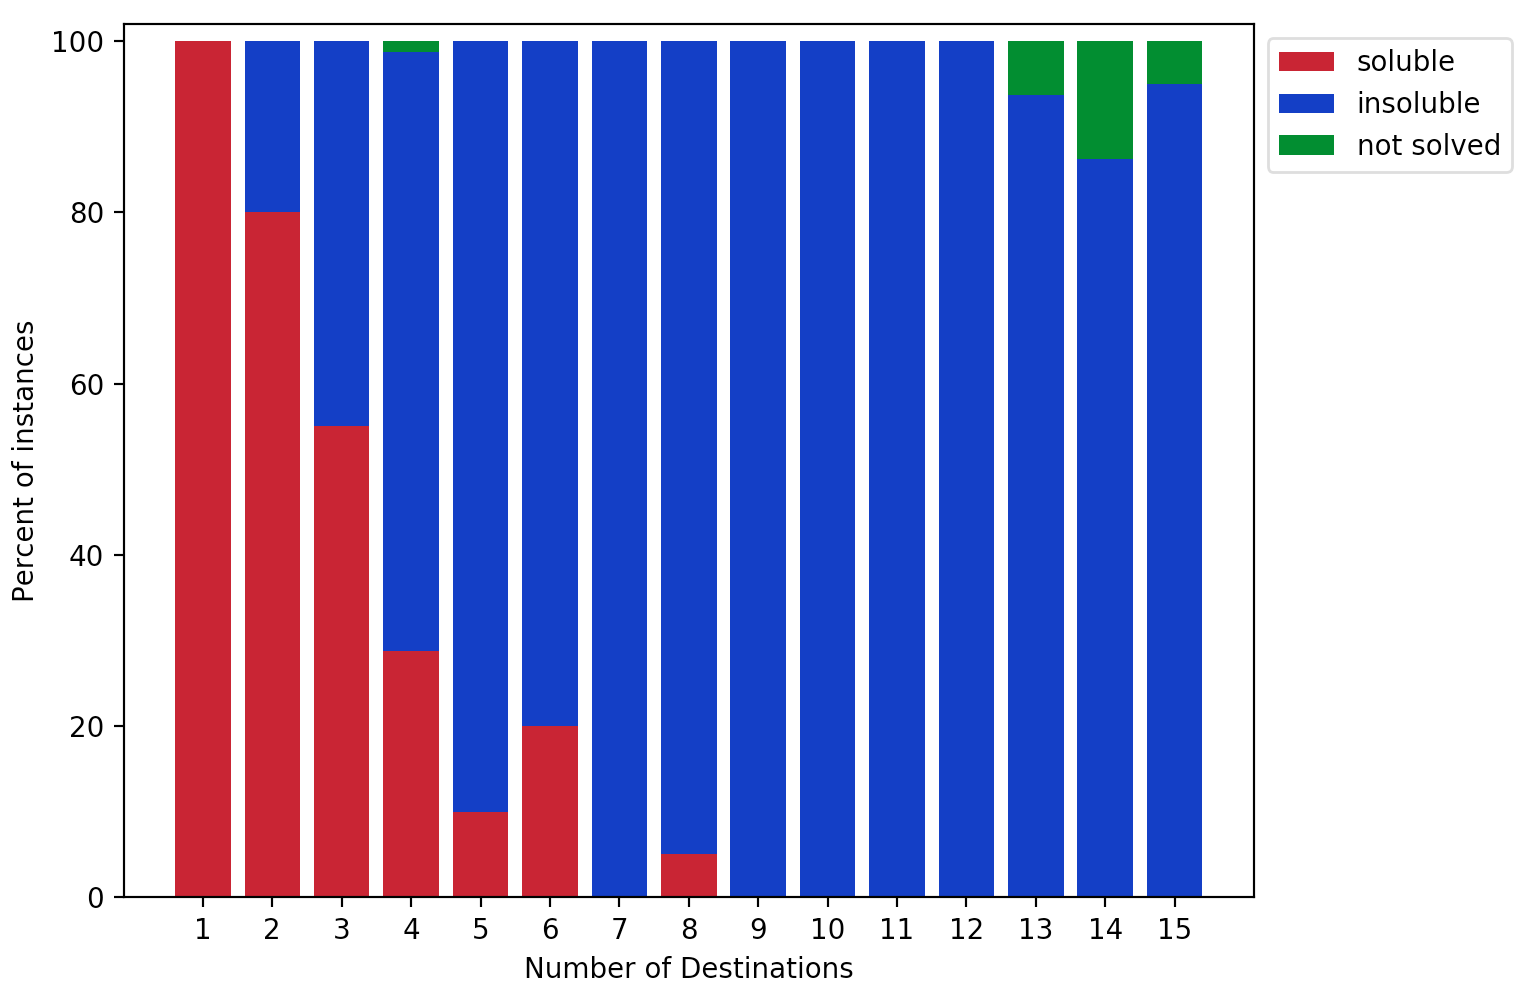
\includegraphics[width=\textwidth, height=5cm]{cpipexperiments/satunsatnotsolved_ip_d.png}
        \caption{IP $\mathcal{D}_3$}
        \label{fig:satunsatnotsolved_ip_d}
    \end{subfigure}
    \caption{The percentage of soluble, insoluble and not solved instances for each setting of $m$, $n$, $d$ and $T$ in dataset $\mathcal{D}_3$ for the IP and CP model.}
    \label{fig:satunsatnotsolved_cp_ip_d}
\end{figure*}

\begin{figure*}
    \centering
    \begin{subfigure}[b]{0.48\textwidth}
        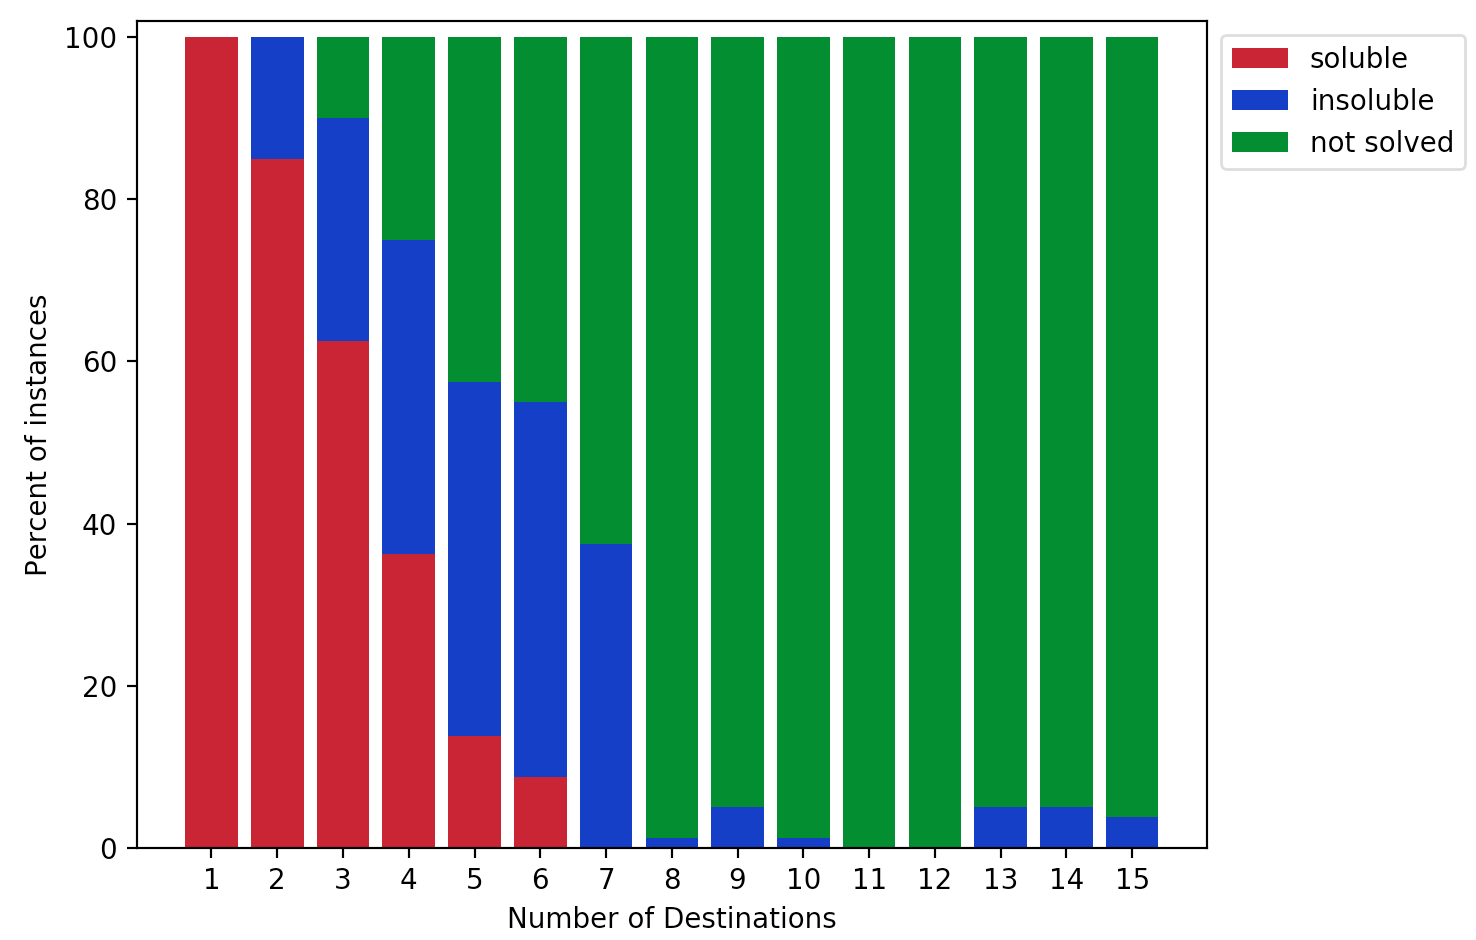
\includegraphics[width=\textwidth, height=5cm]{cpipexperiments/satunsatnotsolved_cp_d2.png}
        \caption{CP $\mathcal{D}_4$}
        \label{fig:satunsatnotsolved_cp_d2}
    \end{subfigure}
    \begin{subfigure}[b]{0.48\textwidth}
        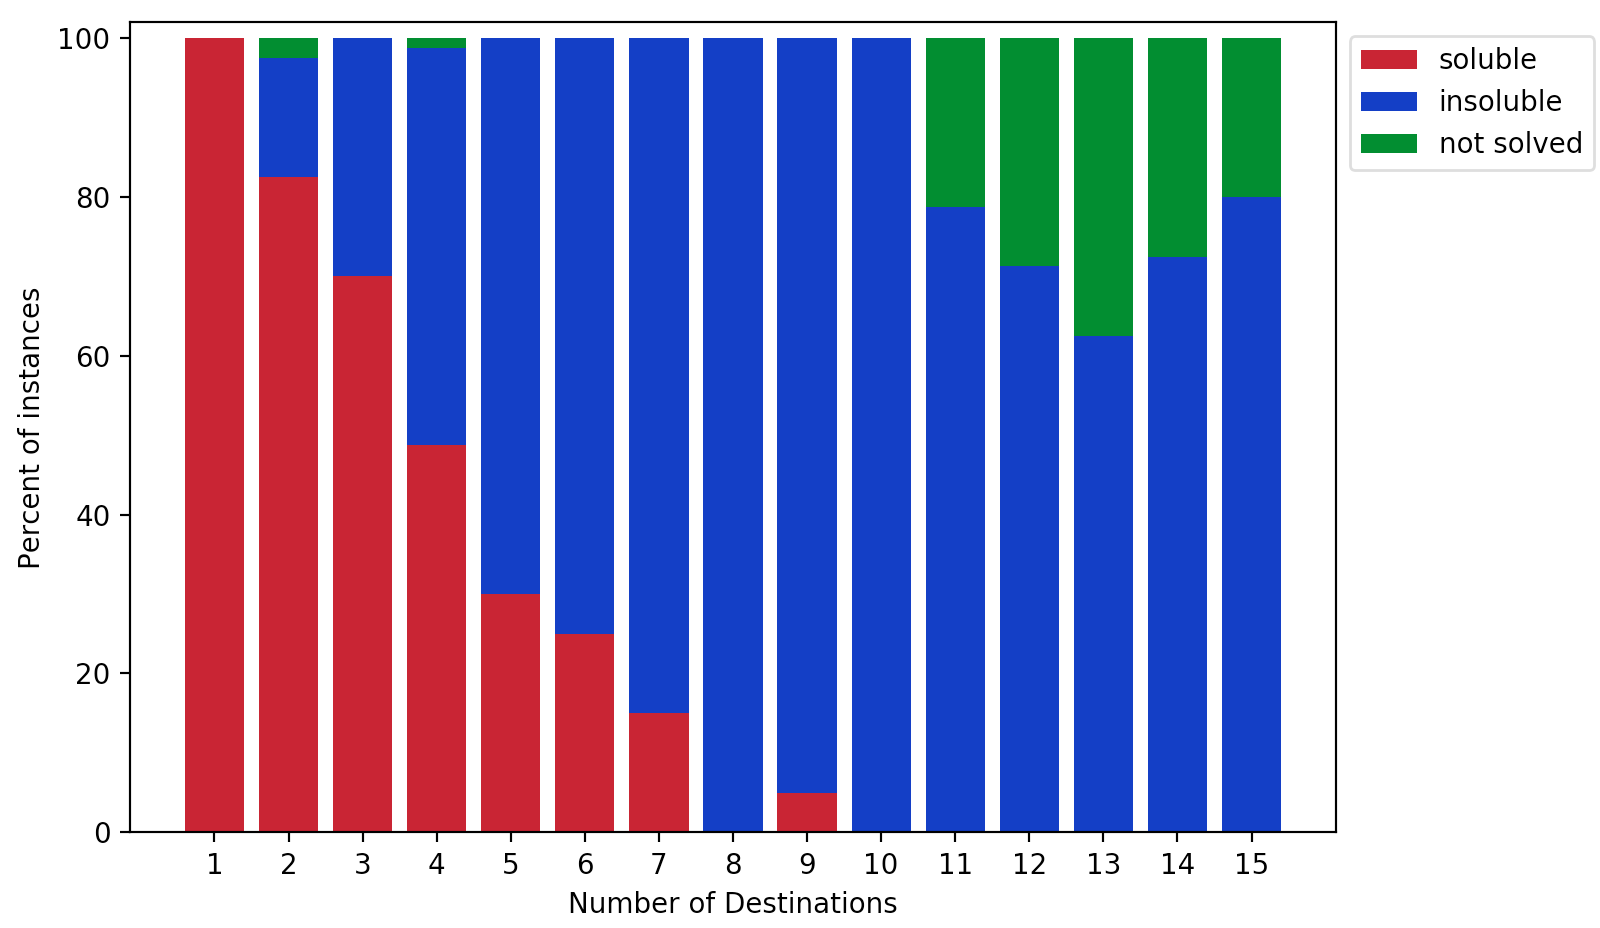
\includegraphics[width=\textwidth, height=5cm]{cpipexperiments/satunsatnotsolved_ip_d2.png}
        \caption{IP $\mathcal{D}_4$}
        \label{fig:satunsatnotsolved_ip_d2}
    \end{subfigure}
    \caption{The percentage of soluble, insoluble and not solved instances for each setting of $m$, $n$, $d$ and $T$ in dataset $\mathcal{D}_4$ for each model.}
    \label{fig:satunsatnotsolved_cp_ip_d2}
\end{figure*}

\subsection{Evaluation of IP}

\textbf{Running time per objective function.} Figures \ref{fig:exp1obj}, \ref{fig:exp2obj}, \ref{fig:exp3obj} and \ref{fig:exp4obj} show the median running time of each objective function for each varied parameter in Experiment 1, 2, 3 and 4 respectively. All four objective functions performed similarly during Experiment 1. For Experiment 2, an unusual rise in the running time of the number of connecting flights objective is observed. Figures \ref{fig:exp3obj} and \ref{fig:exp4obj} show that the trip duration objective has the slowest running time and the rest have similar performance in terms of running time. A reason why trip duration tends to be less fast could be that it involves creating an additional set of variables $y_{i,j}$ and satisfying additional constraints, as presented in Section \ref{subsec:tpip}.

\begin{figure*}
    \centering
    \begin{subfigure}[b]{0.4\textwidth}
        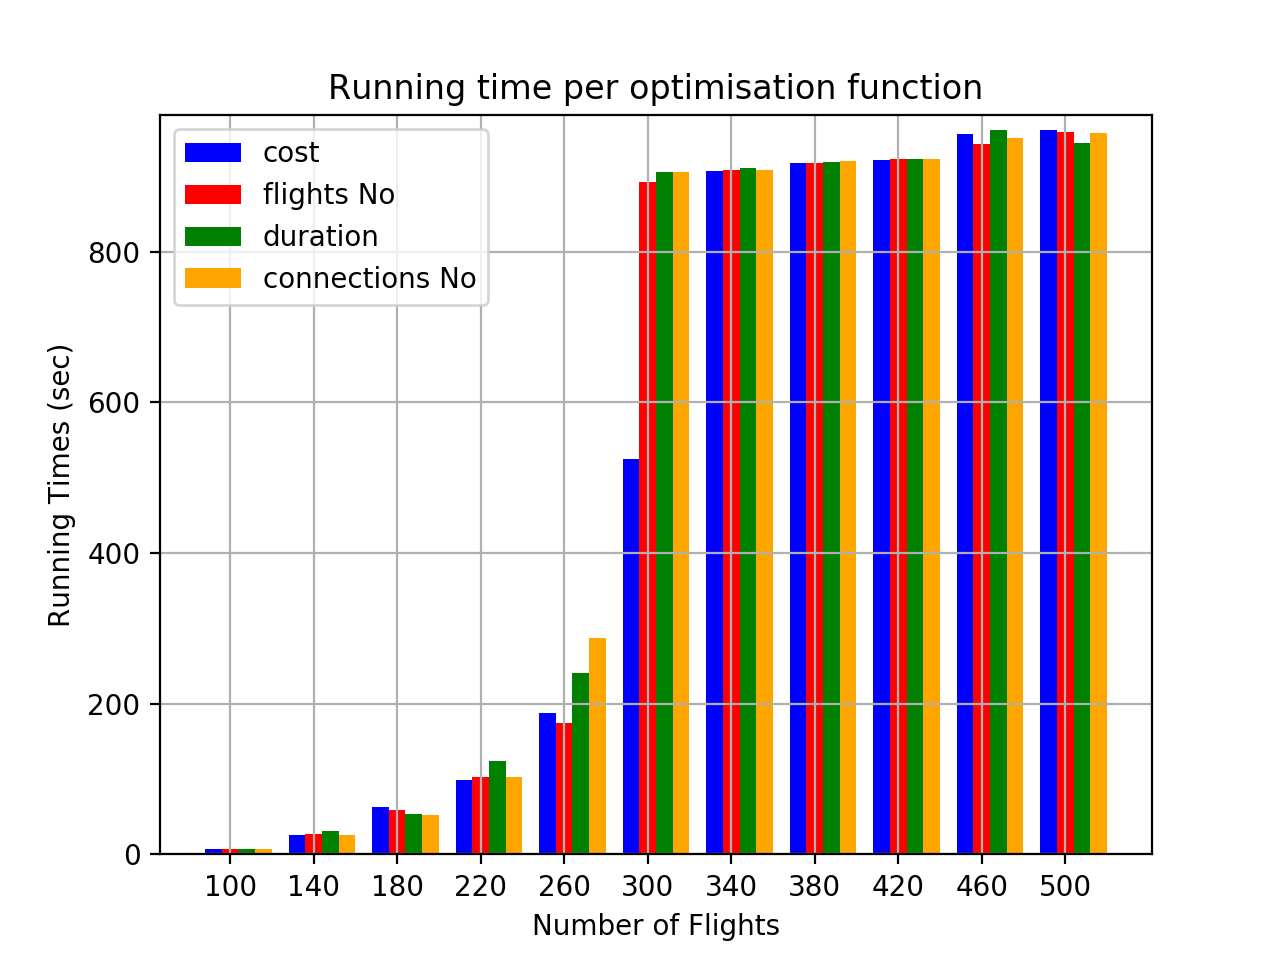
\includegraphics[width=\textwidth]{images/experiments/varym/varyM_obj.png}
        \caption{Experiment 1}
        \label{fig:exp1obj}
    \end{subfigure}
    \begin{subfigure}[b]{0.4\textwidth}
        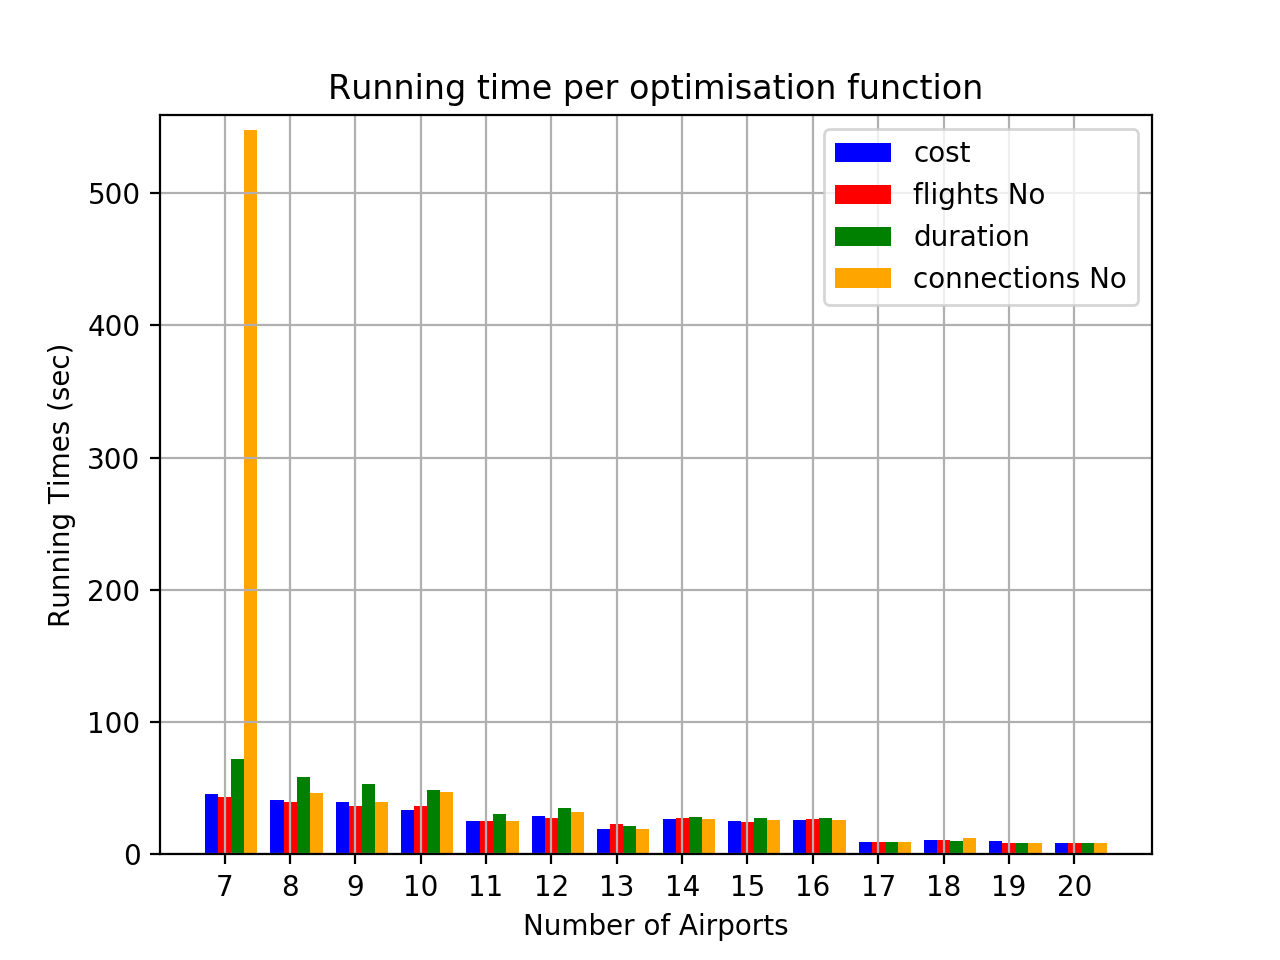
\includegraphics[width=\textwidth]{images/experiments/varyn/varyN_obj.png}
        \caption{Experiment2}
        \label{fig:exp2obj}
    \end{subfigure}
    \begin{subfigure}[b]{0.4\textwidth}
        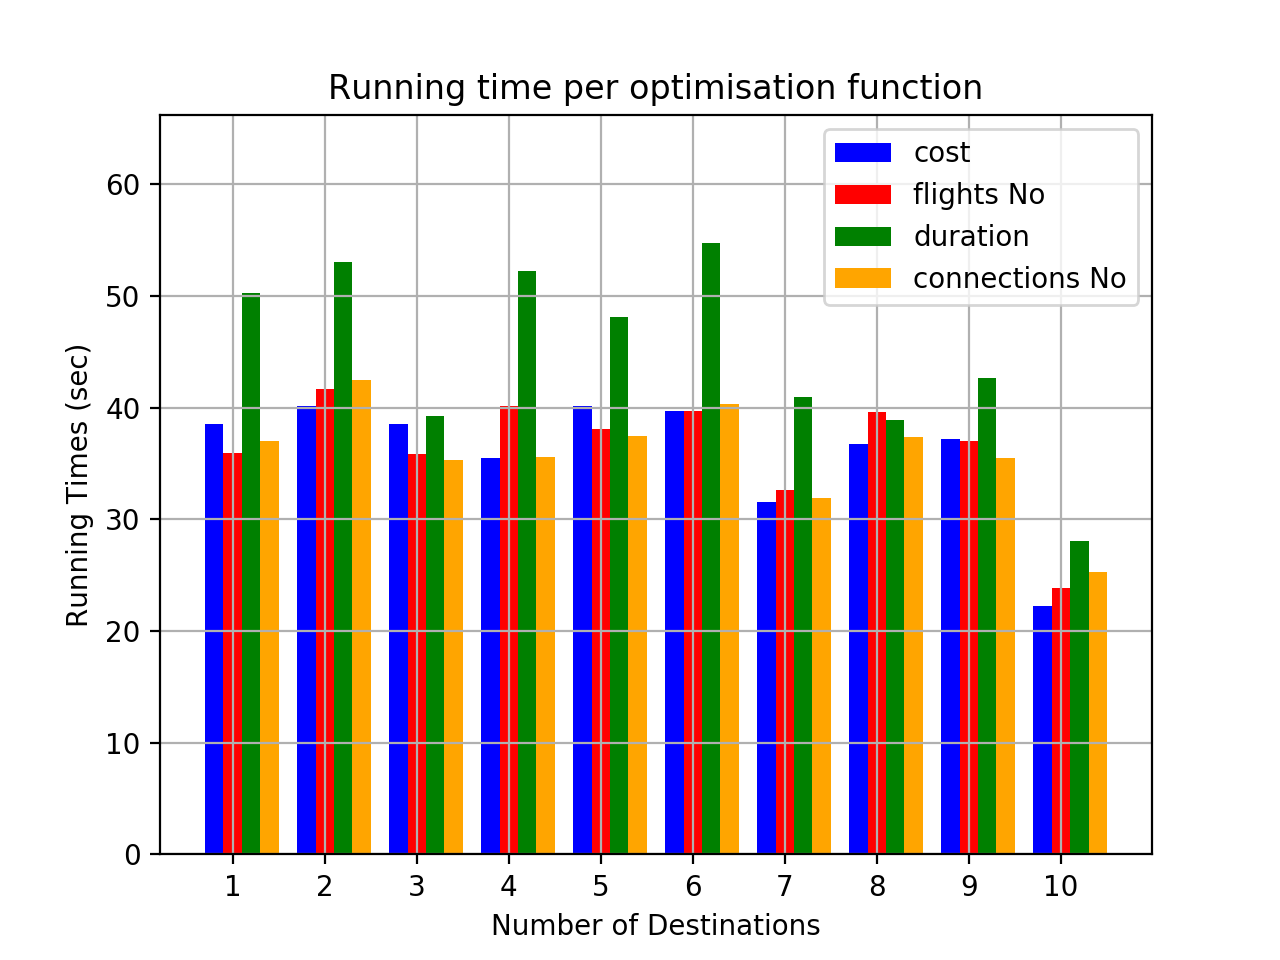
\includegraphics[width=\textwidth]{images/experiments/varyd/varyD_obj.png}
        \caption{Experiment 3}
        \label{fig:exp3obj}
    \end{subfigure}
    \begin{subfigure}[b]{0.4\textwidth}
        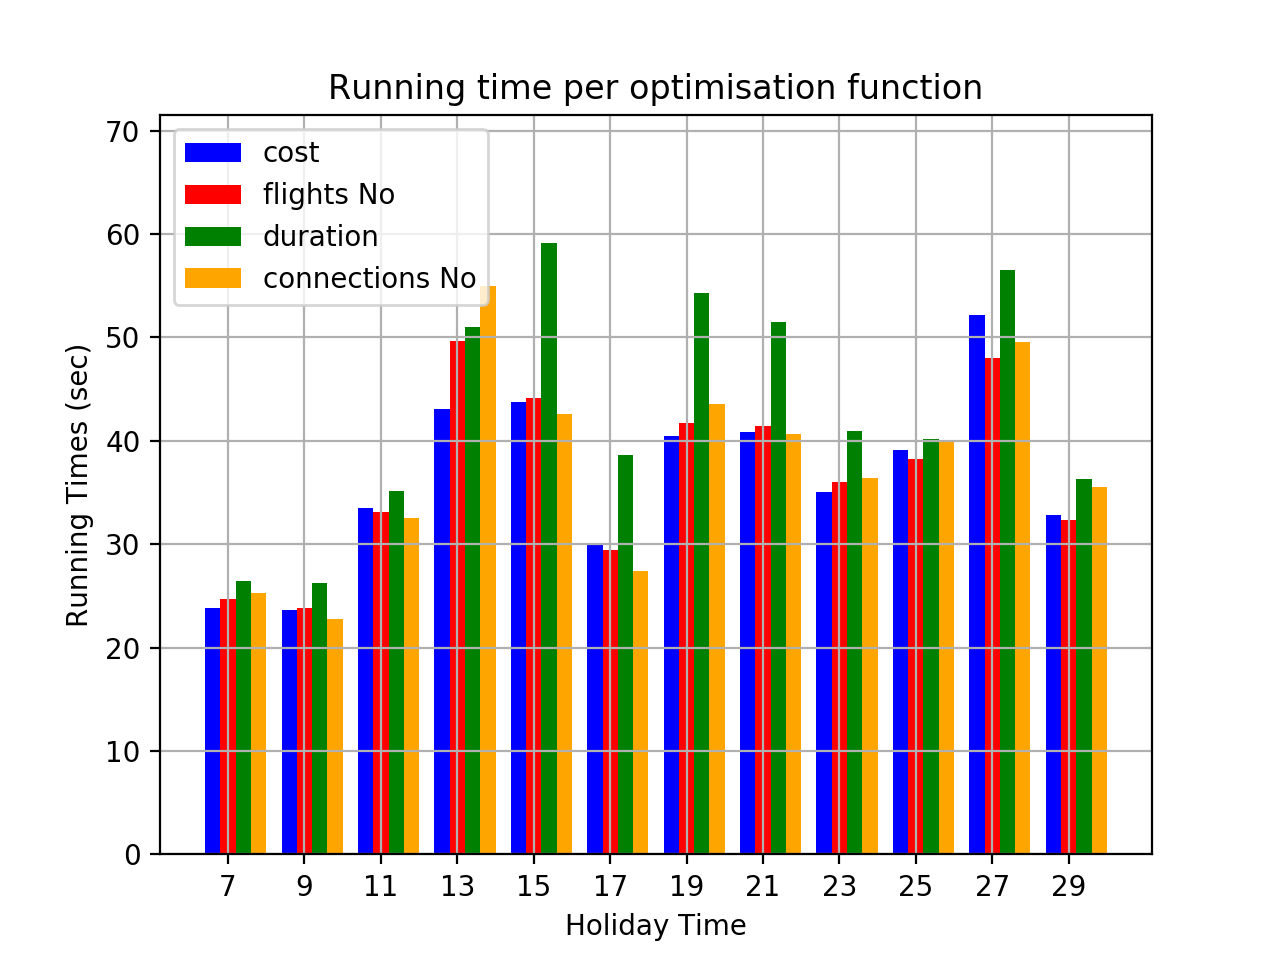
\includegraphics[width=\textwidth]{images/experiments/varyt/varyT_obj.png}
        \caption{Experiment 4}
        \label{fig:exp4obj}
    \end{subfigure}
    \caption{Median running time of each objective for each of the experiments}
\end{figure*}

\end{document}
